% Sumber LaTeX untuk buku ``Metode Aljabar'' dalam bahasa Tionghoa
% Hak cipta 2018 Wen-Wei Li.
% Izin diberikan untuk menyalin, menyebarluaskan, dan/atau mengubah
% dokumen ini berdasarkan ketentuan Creative Commons
% Attribution 4.0 International (CC BY 4.0)
% http://creativecommons.org/licenses/by/4.0/
% Terjemahan Bahasa Indonesia: OpenAI Codex gpt-5.6-sol, Ultra, atas instruksi pengguna.
% Terjemahan independen ini tidak menyiratkan dukungan penulis atau sumber manusia mana pun.

% Untuk disertakan
\chapter{Teori Grup}
Grup merupakan salah satu struktur paling mendasar dalam aljabar. Pokok bahasan bab ini secara garis besar terbagi menjadi dua jenis:
\begin{compactenum}
	\item konstruksi formal, yang mencakup definisi dasar semigrup, monoid, dan grup, serta konsep-konsep seperti aksi grup, produk langsung, dan grup bebas; semuanya juga menjadi landasan untuk mempelajari struktur aljabar lainnya;
	\item sifat-sifat konkret grup itu sendiri, terutama dari sudut pandang kombinatorial, yang mencakup tiga teorema Sylow untuk grup berhingga, grup simetris, serta presentasi grup kepang. Bagian ini kaya akan teknik dan merupakan salah satu daya tarik teori grup.
\end{compactenum}
Kami berupaya merajut kedua jenis bahasan tersebut secara berselang-seling. Untuk konsep dasar teori grup, buku ini tidak memberikan uraian pembedaan yang berkepanjangan. Namun, sifat-sifat formal dan beberapa konstruksi penting yang kerap terlewat dalam buku teks dasar---misalnya grup bebas dan kompletisasi---dibahas secara terperinci sebagai persiapan bagi bab-bab selanjutnya. Adapun pada sisi konkret teori grup, grup simetris merupakan salah satu sumber gagasan bagi teori grup dan teori representasi; \S\ref{sec:symmetric-group} menjadi latihan menyeluruh atas teori yang telah dikembangkan sebelumnya. Klasifikasi grup abelian yang dibangkitkan secara berhingga merupakan hasil penting lain dalam teori grup. Buku ini menanganinya di dalam teori modul; lihat \S\ref{sec:PID-module}.

Walaupun secara logis bab ini hampir mandiri, pembaca diharapkan telah memiliki sedikit pengetahuan dasar tentang grup. Selanjutnya, setiap kali dibahas kategori yang terdiri atas grup, monoid, atau struktur aljabar lain, kecuali dinyatakan berbeda, kita selalu memakai konvensi tentang semesta Grothendieck pada \ref{con:U-small} dan menganggap objek-objek tersebut ``kecil''.

\begin{wenxintishi}
	Materi dari \S\ref{sec:group-and-monoid} sampai \S\ref{sec:group-action} merupakan pengetahuan dasar teori grup; bab ini hanya menempatkannya dalam kerangka yang sedikit lebih luas. Materi setelahnya memerlukan lebih banyak teknik, tetapi tetap bersifat elementer. Bagaimanapun cara konstruksinya, grup bebas yang dibahas dalam \S\ref{sec:free-group} tidak terhindar dari perincian yang agak panjang. Bab ini memulainya dari monoid bebas dan produk teramalgamasi. Argumennya memang lebih panjang, tetapi menghasilkan lebih banyak hal dan juga diperlukan dalam penerapan.

	Seperti telah disebutkan, grup simetris (\S\ref{sec:symmetric-group}) merupakan kelas contoh penting yang harus dibahas. Limit dan kompletisasi (\S\ref{sec:group-limit}) melibatkan bahasa topologi himpunan titik. Materi ini mutlak diperlukan bagi teori Galois tak hingga yang akan dipaparkan kemudian dan merupakan bekal penting untuk penelitian lebih lanjut.

	Salah satu kekurangan bab ini ialah tidak dibahasnya grup simetri rotasi polihedron beraturan, padahal topik tersebut memadukan intuisi geometri dan teknik teori grup dengan indah. Sebagai contoh, grup dodekahedron beraturan dan ikosahedron beraturan saling isomorfik; keduanya merupakan grup sederhana berorde $60$, dan isomorfismenya dengan grup selang-seling $\mathfrak{A}_5$ dapat dinyatakan secara geometris. Pengetahuan tentang materi klasik ini sangat bermanfaat; pembaca disarankan merujuk buku teks terkait, misalnya \cite[Chapter 8]{Har00}.
\end{wenxintishi}

\section{Semigrup, Monoid, dan Grup}\label{sec:group-and-monoid}
Bagian ini mengikuti pendekatan Bourbaki \cite{Bou-Alg1} dalam mendefinisikan struktur aljabar: kita mulai dari himpunan yang dilengkapi suatu \emph{operasi biner}. Operasi biner pada himpunan tak kosong $S$ berarti suatu peta $S \times S \to S$. Biasanya operasi itu ditulis secara multiplikatif sebagai $(x, y) \mapsto x \cdot y$, atau cukup disingkat menjadi $xy$; jadi, operasi biner dapat dipandang sebagai sejenis perkalian pada $S$. Pengulangan operasi menghasilkan ekspresi seperti $x(yz)$ dan $(wx)(yz)$, dengan tanda kurung menunjukkan urutan perkalian unsur-unsurnya. Jika tidak menimbulkan kerancuan, kita sering menghilangkan operasi biner dari notasi struktur $(S, \cdot)$ dan cukup menuliskannya sebagai $S$. Bourbaki memberi struktur yang belum dikenai syarat apa pun ini nama yang tepat, yakni ``magma'' (bahasa Prancis: \emph{le magma}). \index{eryuanyunsuan@operasi biner (binary operation)}

Mula-mula kita kumpulkan beberapa konsep awal tentang $(S, \cdot)$.
\begin{itemize}
	\item Definisikan operasi biner baru $\star$ pada $S$ melalui $x \star y = y \cdot x$. Struktur baru $(S, \star)$ dinotasikan dengan $S^\text{op}$ dan disebut struktur lawan dari $S$.
	\item Jika untuk semua $x,y \in S$ berlaku $xy=yx$, maka $S$ dikatakan memenuhi \emph{hukum komutatif}, atau $S$ dikatakan komutatif; hal ini ekuivalen dengan $S=S^\text{op}$.\index{jiaohuan@komutatif}
	\item Jika $(xy)z=x(yz)$ untuk semua $x,y,z \in S$, maka $S$ dikatakan memenuhi \emph{hukum asosiatif}.
	\item Misalkan $u \in S$. Jika peta \emph{perkalian kiri} yang terkait dari $S$ ke $S$, yakni $x \mapsto ux$, bersifat injektif, maka $u$ dikatakan memenuhi hukum pembatalan kiri. Jika peta \emph{perkalian kanan} $x \mapsto xu$ bersifat injektif, maka $u$ dikatakan memenuhi hukum pembatalan kanan.
	\item Jika $A,B$ merupakan subhimpunan $S$, definisikan
		\[ A B := \{ab : a \in A, \; b \in B \} \subset S; \]
		jika $A$ atau $B$ adalah himpunan tunggal $\{x\}$, maka $AB$ masing-masing ditulis sebagai $xB$ atau $Ax$. Dengan asumsi hukum asosiatif, kita juga dapat mendefinisikan subhimpunan $ABC$, $ABCD$, dan seterusnya tanpa kerancuan.
	\item Jika subhimpunan $A$ dari $S$ memenuhi $AA \subset A$, maka $A$ dikatakan \emph{tertutup terhadap perkalian}.
	\item Unsur $1 \in S$ disebut \emph{unsur identitas} atau unsur satuan jika \index{yaoyuan@unsur identitas (identity element)}
		\[ \forall x \in S, \; x \cdot 1 = 1 \cdot x = x. \]
		Perhatikan bahwa $S$ memiliki paling banyak satu unsur identitas: jika $1,1' \in S$ keduanya unsur identitas, maka $1=1\cdot 1'=1'$. Unsur identitas $S$ juga merupakan unsur identitas $S^\text{op}$. Sejumlah buku menotasikan unsur identitas dengan $e$.
	\item Andaikan terdapat unsur identitas $1$. Untuk $x \in S$, jika terdapat $y \in S$ sedemikian sehingga $yx=1$, maka $x$ disebut invertibel-kiri dan $y$ disebut suatu invers kiri dari $x$; jika syaratnya diganti dengan $xy=1$, kita memperoleh definisi invers kanan dan unsur invertibel-kanan. Unsur yang invertibel-kiri sekaligus invertibel-kanan disebut \emph{unsur invertibel}. Unsur identitas $1$ jelas invertibel.\index{keniyuan@unsur invertibel (invertible element)}
\end{itemize}

\begin{definition}[Semigrup dan monoid]\label{def:monoid}\index{yaobanqun@monoid (monoid)}
	Himpunan tak kosong $S$ yang dilengkapi operasi biner dan memenuhi hukum asosiatif disebut \emph{semigrup}. Semigrup yang memiliki unsur identitas disebut \emph{monoid}. Jika $M$ adalah monoid dan subhimpunan $M' \subset M$ memenuhi
	\begin{inparaenum}[(i)]
		\item $M'$ tertutup terhadap perkalian,
		\item $1 \in M'$,
	\end{inparaenum}
	maka $M'$ disebut submonoid dari $M$.\index{yaobanqun@monoid (monoid)!submonoid}
\end{definition}

Untuk semigrup $S$, hukum asosiatif memastikan bahwa produk berulang dari sembarang unsur $x_1, \ldots, x_n \in S$, yakni $x_1(x_2(\cdots x_n)\cdots)$, dapat ditulis tanpa kerancuan sebagai $x_1 \cdots x_n$; maknanya tidak bergantung pada cara menempatkan tanda kurung. Jika $S$ komutatif, produk berulang ini bahkan tidak bergantung pada urutan $x_1,\ldots,x_n$.

Untuk selanjutnya, misalkan $M$ adalah monoid. Mudah dibuktikan bahwa unsur yang invertibel-kiri (berturut-turut, invertibel-kanan) memenuhi hukum pembatalan kiri (berturut-turut, kanan). Jika $x \in M$ invertibel, maka invers kiri dan invers kanan dari $x$ tunggal dan sama; unsur ini dinotasikan dengan $x^{-1}$. Berikut argumennya: jika $x$ memiliki invers kiri $y$ dan invers kanan $y'$, maka $y'=(yx)y'=y(xy')=y$. Dari sini sekaligus diperoleh ketunggalan invers kiri dan invers kanan serta kesamaan keduanya. Subhimpunan semua unsur invertibel dinotasikan dengan $M^\times$. Subhimpunan ini tertutup terhadap perkalian; bahkan,
\[ \forall x, y \in M^\times, \; (xy)^{-1} = y^{-1} x^{-1}. \]

\begin{definition}[Grup]\label{def:group}\index{qun@grup (group)}\index{qun@grup (group)!orde (order)}
	Monoid yang semua unsurnya invertibel disebut \emph{grup}. Kardinalitas $|G|$ dari grup $G$ disebut \emph{orde} grup tersebut.
\end{definition}

Subhimpunan $M^\times$ dari unsur-unsur invertibel pada sembarang monoid $M$ membentuk sebuah grup terhadap perkalian pada $M$; grup ini disebut grup unit dari $M$\index{danweiqun@grup unit (unit group)}. Berdasarkan pembahasan terdahulu tentang operasi biner, kita dapat mendefinisikan \emph{monoid komutatif} dan \emph{grup komutatif}; yang terakhir juga disebut \emph{grup abelian}. Dengan cara yang sama kita mendefinisikan \emph{monoid lawan} dan \emph{grup lawan}, serta tetap menggunakan notasi $G \mapsto G^\text{op}$.\index[sym1]{G-op@$G^\text{op}$}

Untuk $n \in \Z_{\geq 0}$ dan $x \in M$, kita perkenalkan notasi
\[ x^n := \underbracket{x \cdots x}_{n \text{ faktor }}. \]
Secara khusus, $x^0:=1$, dan untuk unsur invertibel berlaku $(x^{-1})^n=(x^n)^{-1}$; ekspresi terakhir dapat dinotasikan tanpa kerancuan sebagai $x^{-n}$.

\begin{convention}
	Untuk monoid komutatif, lazimnya operasi binernya $\cdot$ ditulis secara aditif sebagai $+$, unsur identitas $1$ ditulis sebagai $0$, dan invers unsur $x$ ditulis sebagai $-x$; meskipun demikian, notasi multiplikatif masih berguna dalam beberapa konteks. Jika diperlukan, hal ini akan dinyatakan secara tersendiri.
\end{convention}

\begin{example}
	Himpunan bilangan real tak negatif $\R_{\geq 0}$ membentuk monoid terhadap penjumlahan, sedangkan $\R_{>0}$ membentuk semigrup. Lebih lanjut, setiap kerucut konveks tertutup $C$ dalam ruang $\R^d$ membentuk monoid terhadap penjumlahan vektor, sedangkan himpunan titik interior dari $C$, yakni $\text{int}(C)$, membentuk semigrup jika tidak kosong. Keduanya komutatif. Dengan meninjau titik-titik kisi di dalam kerucut, kita memperoleh monoid $C \cap \Z^d$ dan semigrup $\text{int}(C) \cap \Z^d$. Di satu sisi, keduanya berhubungan langsung dengan persamaan Diofantin linear dan persoalan kombinatorial seperti pencacahan titik kisi; di sisi lain, keduanya mendefinisikan kelas objek geometri yang disebut varietas torik afin. Struktur monoid komutatif ini jauh lebih kaya daripada struktur grup komutatif yang bersesuaian.
\end{example}

\begin{example}[Grup linear umum]\index[sym1]{GL_n@$\GL(n,F)$}
	Tinjau himpunan $M_n(\R)$ dari semua matriks real berukuran $n \times n$, dan definisikan $\GL(n,\R)$ sebagai subhimpunan yang terdiri atas matriks-matriks invertibel. Jelas bahwa $M_n(\R)$ membentuk monoid terhadap perkalian matriks, dengan matriks identitas sebagai unsur identitasnya, tetapi bukan grup (misalnya, matriks nol tidak invertibel). Di sisi lain, $\GL(n,\R)$ membentuk grup terhadap perkalian matriks; grup ini tepat merupakan grup unit dari $M_n(\R)$. Struktur-struktur ini tidak komutatif apabila $n>1$.
	
	Secara lebih umum, untuk setiap medan $F$ kita tetap dapat mendefinisikan $M_n(F)$ dan $\GL(n,F)$; yang terakhir disebut \emph{grup linear umum} atas $F$. Medan adalah struktur aljabar tempat penjumlahan, pengurangan, perkalian, dan pembagian dapat dilakukan; contohnya mencakup $\Q$, $\R$, dan $\CC$ yang telah dikenal, serta kelas-kelas kongruensi modulo bilangan prima $p$, yakni $\Z/p\Z$. Lihat Definisi \ref{def:field} untuk rinciannya.
\end{example}

\begin{example}[Grup simetris]\label{eg:symmetric-group}\index{duichengqun@grup simetris (symmetric group)}
	Semua bijeksi dari sembarang himpunan $X$ ke dirinya sendiri membentuk sebuah grup, yang disebut \emph{grup simetris} pada $X$ dan dinotasikan dengan $\mathfrak{S}_X:=\Aut(X)$. Operasi binernya ialah komposisi bijeksi $(f,g)\mapsto f\circ g$, unsur identitasnya ialah peta identitas $\identity_X:X\to X$, dan invers setiap unsurnya tidak lain daripada peta invers. Jika $X=\{1,\ldots,n\}$ ($n\in\Z_{\geq 1}$), grup ini juga dinotasikan dengan $\mathfrak{S}_n$ dan disebut grup simetris berderajat $n$, atau grup permutasi. Perhatikan bahwa $|\mathfrak{S}_n|=n!$.
\end{example}
Grup linear umum dan grup simetris merupakan dua kelas contoh penting dalam teori grup; pembaca hendaknya mengingat keduanya.

\begin{definition}[Subgrup dan subgrup normal]\index{ziqun@subgrup (subgroup)}\index{zhengguiziqun@subgrup normal (normal subgroup)}
	Misalkan $G$ adalah grup. Subhimpunan $H \subset G$ disebut \emph{subgrup} dari $G$ jika
	\begin{inparaenum}[(i)]
		\item $H$ adalah submonoid,
		\item $x^{-1}\in H$ untuk setiap $x\in H$.
	\end{inparaenum}
	Jika subgrup $H$ memenuhi $xH=Hx$ untuk semua $x\in G$, maka $H$ disebut \emph{subgrup normal} dari $G$, dan kita tulis $H\lhd G$. Subgrup $\{1\}\lhd G$ disebut \emph{subgrup trivial} dari $G$.
\end{definition}
Definisi subgrup normal dapat ditulis kembali sebagai $\forall x\in G,\;xHx^{-1}=H$. Karena $xHx^{-1}=H$ ekuivalen dengan $xHx^{-1}\subset H$ dan $x^{-1}Hx\subset H$, untuk memeriksa kenormalan cukup dibuktikan bahwa $xHx^{-1}\subset H$ bagi setiap $x$. Galois adalah orang pertama yang memahami pentingnya subgrup normal.

\begin{definition}[Grup sederhana]\index{qun@grup (group)!sederhana (simple)}
	Jika grup $G$ tidak mempunyai subgrup normal selain $\{1\},G$, maka $G$ disebut \emph{grup sederhana}.
\end{definition}
Grup selang-seling $\mathfrak{A}_n$ ($n\geq 5$) merupakan keluarga pertama grup sederhana berhingga nonkomutatif yang ditemukan; hal ini akan dijelaskan secara terperinci dalam Teorema \ref{prop:A_n-simple}. Klasifikasi grup sederhana berhingga hingga isomorfisme merupakan tonggak besar dalam perkembangan teori grup. Sejak Hölder mengajukan masalah klasifikasi ini pada 1892 hingga Aschbacher dan Smith menyelesaikan bagian terakhir pembuktian Gorenstein dan para kolaboratornya sekitar 2004, pengerjaannya memakan waktu lebih dari satu abad. Literatur terkait sangat luas; bahkan gambaran kasar atas hasil klasifikasinya memerlukan ruang yang tidak sedikit. Pembaca yang berminat dipersilakan merujuk \cite{Wil09}.

Irisan subgrup-subgrup tetap merupakan subgrup, dan irisan subgrup-subgrup normal tetap normal. Misalkan $E\subset G$ adalah sembarang subhimpunan. Subgrup terkecil yang memuat $E$ disebut subgrup yang \emph{dibangkitkan} oleh $E$ dan dinotasikan dengan $\lrangle{E}$. Unsur-unsurnya adalah semua unsur yang dapat diperoleh dari unsur-unsur $E$ dengan perkalian dan pengambilan invers. Salah satu cara langsung untuk menuliskannya ialah \index[sym1]{<E>@$\lrangle{E}$}
\[ \lrangle{E} := \bigcap_{\substack{H \subset G: \text{subgrup} \\ H \supset E}} H. \]
Demikian pula, subgrup normal yang dibangkitkan oleh $E$ didefinisikan sebagai $\bigcap_{E \subset N \lhd G}N$. Jika $E$ adalah himpunan tunggal $\{x\}$, kita memakai singkatan
\[ \lrangle{x} := \lrangle{\{x\}} = \{ x^n : n \in \Z \}. \]
Untuk sembarang $G$ dan $x\in G$, kita tulis $\ord(x):=|\lrangle{x}|$ dan menyebutnya \emph{orde} dari $x$.\index[sym1]{ordx@$\ord(x)$} \index{qun@grup (group)!orde (order)}

\begin{definition}[Grup siklik]\label{def:cyclic-group}\index{xunhuanqun@grup siklik (cyclic group)}
	Jika terdapat unsur $x$ dalam grup $G$ sedemikian sehingga $G=\lrangle{x}$, maka $G$ disebut grup siklik. Dengan kata lain, grup siklik adalah grup yang dapat dibangkitkan oleh satu unsur. Lihat Contoh \ref{eg:cyclic-group}.
\end{definition}

\begin{example}\label{eg:Z-as-group}
	% O013-LI-U025-COR-001: pembatas ambien G pada sumber dikoreksi menjadi \Z; lihat tinjauan QA Unit 025.
	Himpunan semua bilangan bulat $\Z$ membentuk grup terhadap penjumlahan. Grup ini dibangkitkan oleh $1\in\Z$ dan karena itu siklik. Semua subgrup $H\subset\Z$ berbentuk $H=n\Z=\{m\in\Z:n\mid m\}$: jika $H\neq\{0\}$, cukup ambil $n$ sebagai unsur terkecil dari $H\cap\Z_{>0}$.
\end{example}

\begin{definition}[Koset]\label{def:coset}\index{peiji@koset (coset)}
	Misalkan $H$ adalah subgrup dari grup $G$. Definisikan:
	\begin{compactitem}
		\item koset kiri: subhimpunan $G$ yang berbentuk $xH$; himpunan semua koset kiri dinotasikan dengan $G/H$;
		\item koset kanan: subhimpunan $G$ yang berbentuk $Hx$; himpunan semua koset kanan dinotasikan dengan $H \backslash G$;
		\item koset ganda: jika $K$ adalah subgrup lain, maka subhimpunan $G$ yang berbentuk $HxK:=\{hxk:h\in H,k\in K\}$ disebut koset ganda dari $G$ terhadap $(H,K)$; himpunan semua koset ganda dinotasikan dengan $H\backslash G/K$.
	\end{compactitem}
	Unsur suatu koset disebut suatu wakil dari koset tersebut. Jika $H\lhd G$, tidak ada perbedaan antara koset kiri dan kanan. Karena sisi suatu koset selalu tampak dari notasinya, selanjutnya kita tidak akan menyebutkannya lagi. Definisikan indeks $H$ dalam $G$ sebagai
	\[ (G:H) := |G/H|. \]
	Ruang koset $G/H$ tidak harus berhingga; di sini $(G:H)$ dipandang sebagai suatu kardinal. \index[sym1]{G:H@$(G:H)$}
\end{definition}
Koset kiri dan kanan sebenarnya merupakan kasus khusus koset ganda, dengan masing-masing mengambil $H$ atau $K$ sama dengan $\{1\}$. Karena itu, hasil berikut hanya dirumuskan untuk koset ganda.
\begin{lemma}\label{prop:coset-decomp}
	Misalkan $H,K$ adalah subgrup dari grup $G$. Maka,
	\begin{compactenum}[(i)]
		\item untuk sembarang koset ganda $HxK$ dan $HyK$, irisannya tak kosong jika dan hanya jika $HxK=HyK$;
		\item $G$ dapat ditulis sebagai gabungan saling lepas $G=\bigsqcup_x HxK$, dengan memilih satu wakil $x$ dari setiap koset ganda dalam $H\backslash G/K$.
	\end{compactenum}
\end{lemma}
\begin{proof}
	Andaikan $HxK\cap HyK\neq\emptyset$. Jika $hxk=h'yk'$, maka $x=h^{-1}h'yk'k^{-1}\in HyK$, sehingga $HxK\subset HHyKK=HyK$; oleh simetri, $HyK\subset HxK$, dan karenanya keduanya sama. Karena setiap $g\in G$ termuat dalam $HgK$, pernyataan tentang gabungan saling lepas tersebut langsung diperoleh.
\end{proof}

Untuk setiap $x\in G$, perkalian kiri $h\mapsto xh$ memberikan bijeksi himpunan $H\to xH$, sebab unsur-unsur grup memenuhi hukum pembatalan kiri. Demikian pula, perkalian kanan memberikan bijeksi $H\to Hx$.

\begin{proposition}\label{prop:Lagrange}
	Misalkan $H$ adalah subgrup dari grup $G$. Maka,
	\begin{compactenum}[(i)]
		\item $|G|=(G:H)|H|$; khususnya, jika $G$ berhingga, maka $|H|$ membagi $|G|$ (disebut teorema Lagrange);
		\item jika $K$ adalah subgrup dari $H$, maka $(G:K)=(G:H)(H:K)$.
	\end{compactenum}
	Hasil kali di sini adalah hasil kali kardinal.
\end{proposition}
\begin{proof}
	Dekomposisi koset
	\begin{align*}
		H &= \bigsqcup_y yK, \\
		G &= \bigsqcup_x xH = \bigsqcup_{x,y} xyK
	\end{align*}
	dapat digunakan untuk membuktikan (ii). Karena $(G:1)=|G|$ dan $(H:1)=|H|$, dengan mengambil $K=\{1\}$ kita memperoleh (i).
\end{proof}

\begin{definition}[Pusat, sentralisator, dan normalisator]\index{zhongxin@pusat}\index[sym1]{Z_G@$Z_G$}\index[sym1]{N_G(E)@$N_G(\cdot)$}\index[sym1]{Z_G(E)@$Z_G(\cdot)$}
	Misalkan $G$ adalah grup.
	\begin{compactenum}[(i)]
		\item \emph{Pusat} dari $G$ didefinisikan sebagai $Z_G:=\{z\in G:\forall x\in G,\;xz=zx\}$;
		\item jika $E\subset G$ adalah sembarang subhimpunan, \emph{sentralisatornya} didefinisikan sebagai $Z_G(E):=\{z\in G:\forall x\in E,\;xz=zx\}$;
		\item dengan notasi yang sama, \emph{normalisatornya} didefinisikan sebagai $N_G(E):=\{n\in G:nEn^{-1}=E\}$.
	\end{compactenum}
	Jika $E$ adalah himpunan tunggal $\{x\}$, kita memakai singkatan $Z_G(x)$ dan $N_G(x)$.
\end{definition}

Jelas bahwa $Z_G(E)$ dan $N_G(E)$ keduanya merupakan subgrup, dan $Z_G(E)\lhd N_G(E)$. Subgrup yang pertama hanya bergantung pada subgrup $\lrangle{E}$ yang dibangkitkan oleh $E$. Jika $H$ adalah subgrup, maka $H\lhd N_G(H)$. Dengan mengambil $E=G$, diperoleh
\[ Z_G(G) = Z_G \lhd G = N_G(G). \]

\begin{remark}\label{rem:HN}
	Jika $N,H\subset G$ merupakan subgrup dan $H\subset N_G(N)$, maka $HN=NH$ merupakan subgrup dari $G$ dan $N\lhd HN$. Pembaca diminta memeriksanya sendiri.
\end{remark}
\section{Homomorfisme dan grup hasil bagi}\label{sec:homomorphism}
Makna homomorfisme adalah peta pelestari struktur. Untuk himpunan tak kosong $S_1, S_2$ yang dilengkapi operasi biner, struktur yang harus dilestarikan oleh homomorfisme $\varphi: S_1 \to S_2$ tidak lain adalah operasi biner tersebut, yakni $\forall x,y \in S_1, \; \varphi(xy)=\varphi(x)\varphi(y)$. Dengan gagasan ini kita dapat mendefinisikan homomorfisme semigrup. Namun, kasus monoid lebih umum dijumpai dan lebih berguna; dalam hal ini kita mensyaratkan agar homomorfisme melestarikan perkalian sekaligus unsur identitas.\index{homomorfisme@homomorfisme (homomorphism)}

\begin{definition}[Homomorfisme dan isomorfisme]
	Misalkan $M_1, M_2$ adalah monoid. Suatu peta $\varphi: M_1 \to M_2$ disebut \emph{homomorfisme} apabila memenuhi sifat-sifat berikut.
	\begin{compactenum}[(i)]
		\item $\forall x,y \in M_1, \; \varphi(xy) = \varphi(x) \varphi(y)$;
		\item $\varphi(1)=1$.
	\end{compactenum}
	Homomorfisme dari monoid $M$ ke dirinya sendiri disebut \emph{endomorfisme}; contohnya ialah peta identitas $\identity_M: M \to M$. Komposisi homomorfisme tetap merupakan homomorfisme. Homomorfisme bernilai konstan $1$ disebut \emph{homomorfisme trivial}.\index{endomorfisme@endomorfisme (endomorphism)}

	Jika terdapat homomorfisme $\psi: M_2 \to M_1$ sedemikian sehingga $\varphi \psi = \identity_{M_2}$ dan $\psi \varphi = \identity_{M_1}$, maka $\varphi$ disebut invertibel dan $\psi$ disebut invers dari $\varphi$; homomorfisme invertibel disebut \emph{isomorfisme}, dan ditulis $\varphi: M_1 \rightiso M_2$. Dalam hal ini kita juga mengatakan bahwa $M_1$ dan $M_2$ isomorfik. Isomorfisme dari suatu monoid ke dirinya sendiri disebut \emph{automorfisme}.\index{isomorfisme}\index{automorfisme@automorfisme (automorphism)}
\end{definition}

Himpunan semua homomorfisme dari $M_1$ ke $M_2$ ditulis $\Hom(M_1, M_2)$. Sifat-sifat berikut jelas:
\begin{compactitem}
	\item invers dari $\varphi: M_1 \to M_2$, jika ada, bersifat tunggal dan ditulis $\varphi^{-1}$;
	\item $\varphi$ invertibel jika dan hanya jika $\varphi$ merupakan bijeksi;
	\item $\varphi$ menginduksi peta antara grup unit $M_1^\times \to M_2^\times$. Sesungguhnya, $\forall x \in M_1^\times, \;\varphi(x)^{-1} = \varphi(x^{-1})$;
	\item untuk setiap monoid $M$, semua endomorfismenya, terhadap komposisi peta $\circ$, membentuk monoid $\End(M) := \Hom(M, M)$; grup unit dari monoid tersebut, yaitu $\Aut(M)$, merupakan \emph{grup automorfisme} $M$ dan, sesuai namanya, terdiri atas automorfisme.
\end{compactitem}

Kita telah mendefinisikan konsep homomorfisme untuk monoid. Grup merupakan kasus khusus monoid; homomorfisme antara grup juga disebut \emph{homomorfisme grup}. Isomorfisme grup, automorfisme grup, dan konsep-konsep serupa didefinisikan dengan cara yang sama. Dalam kasus grup, definisi homomorfisme juga mempunyai penyederhanaan berikut, yang sangat memudahkan perhitungan dan selanjutnya akan kita gunakan tanpa keterangan tambahan.
\begin{proposition}
	Misalkan $G_1$, $G_2$ adalah grup. Peta $\varphi: G_1 \to G_2$ merupakan homomorfisme grup jika dan hanya jika untuk semua $x, y \in G_1$ berlaku $\varphi(xy)=\varphi(x)\varphi(y)$.
\end{proposition}
\begin{proof}
	Bagian penting adalah arah ``jika''. Dari $\varphi(1)\varphi(1) = \varphi(1 \cdot 1) = \varphi(1)$, kalikan kedua ruas dari kiri dengan $\varphi(1)^{-1}$ untuk memperoleh $\varphi(1) = 1$.
\end{proof}

Ada satu jenis automorfisme grup yang sangat umum, yang disebut \emph{automorfisme dalam} atau \emph{automorfisme adjoin}: untuk grup $G$ dan $x \in G$, definisikan automorfisme\index{automorfisme!automorfisme dalam (inner automorphism)}
\begin{align*}
	\Ad_x: G & \longrightarrow G \\
	g & \longmapsto {}^x g := xgx^{-1}.
\end{align*}
Mudah diperiksa bahwa $\Ad_1 = \identity_G$ dan $\Ad_{xy} = \Ad_x \circ \Ad_y$, sehingga selanjutnya kita memperoleh homomorfisme grup
\begin{align*}
	\Ad: G & \longrightarrow \Aut(G) \\
	x & \longmapsto \Ad_x.
\end{align*}

\begin{definition}
	Misalkan $\varphi: G_1 \to G_2$ adalah homomorfisme grup. Bayangannya ditulis $\Image(\varphi) := \{\varphi(x) : x \in G_1\}$, sedangkan \emph{kernelnya} didefinisikan sebagai \index{kernel@kernel (kernel)}\index[sym1]{Ker@$\Ker$}
	\[ \Ker(\varphi) := \varphi^{-1}(1). \]
\end{definition}
Langsung dari definisi diperoleh bahwa $\Image(\varphi)$ merupakan subgrup dari $G_2$, sedangkan $\Ker(\varphi)$ merupakan subgrup normal dari $G_1$. Sebagai contoh, pusat grup $Z_G$ dapat dideskripsikan sebagai kernel $\Ker\left[ \Ad: G \to \Aut(G) \right]$.

Sekarang saatnya kembali menelaah struktur hasil bagi. Misalkan $S$ adalah himpunan tak kosong dan $\sim$ adalah relasi ekuivalensi pada $S$; kelas-kelas ekuivalensi yang bersesuaian membentuk himpunan hasil bagi $S/\sim$. Kelas ekuivalensi yang memuat unsur $x \in S$ ditulis $[x]$. Pertanyaan umum yang menjadi perhatian matematikawan ialah: bagaimana $S/\sim$ dapat mewarisi struktur aljabar, topologi, atau struktur lain dari $S$? Di sini kita anggap $S$ dilengkapi operasi biner. Yang dimaksud dengan mewarisi ialah bahwa peta hasil bagi $x \mapsto [x]$ melestarikan operasi biner; dengan kata lain, kita menghendaki persamaan
\[ [x] \cdot [y] = [x \cdot y], \quad x,y \in S \]
berlaku dalam $S/\sim$. Jelas bahwa persamaan ini mencirikan secara tunggal operasi biner pada $S/\sim$. Persoalannya adalah apakah operasi tersebut terdefinisi dengan baik. Setelah merenungkannya sejenak, pembaca akan melihat bahwa kita harus menambahkan syarat
\begin{gather}\label{eqn:quotient-condition}
	(x \sim x') \wedge (y \sim y') \implies xy \sim x'y', \quad x,x',y,y' \in S.
\end{gather}

Struktur $S/\sim$ yang didefinisikan demikian disebut \emph{struktur hasil bagi}. Jika $S$ merupakan semigrup (atau monoid, atau grup), maka demikian pula $S/\sim$; dalam dua kasus terakhir, unsur identitas $S/\sim$ adalah $[1]$, sedangkan khusus dalam kasus grup, invers setiap unsur diberikan oleh $[x]^{-1} = [x^{-1}]$. Berikutnya, tinjau kasus monoid $M$. Untuk relasi ekuivalensi pada $M$ yang memenuhi \eqref{eqn:quotient-condition}, katakanlah $\sim$, peta $x \mapsto [x]$ memberikan homomorfisme $M \to M/\sim$. Monoid hasil bagi $M/\sim$ memenuhi sifat berikut.

\begin{proposition}\label{prop:quotient-monoid-univ-prop}
	Untuk setiap homomorfisme $\varphi: M \to M'$ yang memenuhi $(x \sim y) \implies \varphi(x)=\varphi(y)$, terdapat homomorfisme tunggal $\bar{\varphi}: (M/\sim) \to M'$ yang membuat diagram berikut komutatif.
	\[ \begin{tikzcd}
		M \arrow[r, "\varphi"] \arrow[d] & M' \\
		M/\sim \arrow[ru, "{\exists! \bar{\varphi}}"'] &
	\end{tikzcd} \]
\end{proposition}
Homomorfisme $\bar{\varphi}$ ini disebut homomorfisme terimbas oleh $\varphi$. Diagram komutatif berarti bahwa komposisi $\bar{\varphi}$ dengan $M \to M/\sim$ sama dengan $\varphi$; lihat pembahasan dalam \S\ref{sec:cat-and-morphism}.
\begin{proof}
	Satu-satunya pilihan ialah $\bar{\varphi}([x]) = \varphi(x)$, dengan $x \in M$.
\end{proof}

\begin{proposition}\label{prop:1st-homomorphism-monoid}
	Misalkan $\varphi: M \to M'$ adalah homomorfisme surjektif. Definisikan relasi ekuivalensi pada $M$ dengan $x \sim y \iff \varphi(x)=\varphi(y)$. Maka $\sim$ memenuhi \eqref{eqn:quotient-condition}, dan homomorfisme terimbas $\bar{\varphi}: (M/\sim) \to M'$ merupakan isomorfisme.
\end{proposition}
\begin{proof}
	Syarat \eqref{eqn:quotient-condition} langsung terlihat. Dari definisi $\sim$ diketahui bahwa $\bar{\varphi}$ merupakan bijeksi, sehingga merupakan isomorfisme.
\end{proof}

Untuk grup $G$, relasi ekuivalensi yang memenuhi syarat \eqref{eqn:quotient-condition} mempunyai deskripsi yang lebih sederhana. Definisikan $N := \{x \in G : 1 \sim x\}$. Maka
\begin{gather}\label{eqn:quotient-condition-group}
	(x \sim y) \iff \left( x^{-1} y \in N \right).
\end{gather}
Jadi relasi ekuivalensi $\sim$ sepenuhnya ditentukan oleh himpunan bagian $N$. Sebaliknya, untuk suatu himpunan bagian $N$, dapat diperiksa langsung bahwa \eqref{eqn:quotient-condition-group} mendefinisikan relasi ekuivalensi jika dan hanya jika $N$ memuat $1$ serta tertutup terhadap invers dan perkalian, yakni jika dan hanya jika $N$ merupakan subgrup. Relasi ini memenuhi \eqref{eqn:quotient-condition} jika dan hanya jika $N$ merupakan subgrup normal. Kita memperoleh bijeksi berikut (ingat Definisi \ref{def:coset}):
\begin{align*}
	G/\sim & \stackrel{\sim}{\longrightarrow} G/N \\
	[x] & \longmapsto xN = Nx.
\end{align*}
Hal ini menjelaskan definisi grup hasil bagi berikut.

\begin{definition}[Grup hasil bagi]\index{hasil bagi}
	Misalkan $G$ adalah grup dan $N$ adalah subgrup normalnya. Pada ruang koset $G/N$, definisikan operasi biner
	\[ xN \cdot yN = xy N, \quad x,y \in G. \]
	Dengan operasi ini, $G/N$ membentuk grup yang disebut \emph{grup hasil bagi} $G$ modulo $N$; unsur identitasnya adalah $1 \cdot N$, sedangkan invers diberikan oleh $(xN)^{-1} = x^{-1}N$. Homomorfisme grup
	\begin{align*}
		\pi: G & \longrightarrow G/N \\
		x & \longmapsto xN
	\end{align*}
	disebut homomorfisme hasil bagi.
\end{definition}
Perhatikan bahwa homomorfisme hasil bagi $\pi: G \to G/N$ selalu surjektif, dan $\Ker(\pi) = N$. Sekarang kita dapat menyatakan beberapa sifat dasar homomorfisme.

\begin{proposition}\label{prop:1st-homomorphism}
	Misalkan $\varphi: G_1 \to G_2$ adalah homomorfisme grup. Maka $\varphi$ menginduksi isomorfisme $\bar{\varphi}: G_1/\Ker(\varphi) \rightiso \Image(\varphi)$ yang memetakan koset $g \cdot \Ker(\varphi)$ ke $\varphi(g)$.
\end{proposition}
\begin{proof}
	Terapkan Proposisi \ref{prop:1st-homomorphism-monoid}.
\end{proof}

\begin{proposition}\label{prop:2nd-homomorphism}
	Misalkan $\varphi: G_1 \to G_2$ adalah homomorfisme surjektif antara grup. Maka terdapat bijeksi
	\[ \begin{tikzcd}[row sep=small]
		\left\{ \text{subgrup }  H_2 \subset G_2  \right\} \arrow[leftrightarrow, r, "1:1"] & \left\{ \text{subgrup } H_1 \subset G_1 : H_1 \supset \Ker(\varphi)  \right\} \\
		\left\{ \text{subgrup normal }  H_2 \lhd G_2  \right\} \arrow[phantom, u, "\subset" description, sloped] \arrow[leftrightarrow, r, "1:1"] & \left\{ \text{subgrup normal } H_1 \lhd G_1 : H_1 \supset \Ker(\varphi)  \right\} \arrow[phantom, u, "\subset" description, sloped] \\
		H_2 \arrow[mapsto, r] & \varphi^{-1}(H_2) \\
		\varphi(H_1) & H_1 \arrow[mapsto, l] .
	\end{tikzcd} \]
	Bijeksi ini memenuhi $H_2 \subset H'_2 \iff \varphi^{-1}(H_2) \subset \varphi^{-1}(H'_2)$. Selain itu, morfisme komposit $G_1 \xrightarrow{\varphi} G_2 \twoheadrightarrow G_2/H_2$ menginduksi isomorfisme $G_1/\varphi^{-1}(H_2) \rightiso G_2/H_2$.
\end{proposition}
Ketika $\varphi$ adalah homomorfisme hasil bagi $G \twoheadrightarrow G/N$, isomorfisme dalam pernyataan tersebut dapat ditulis dalam bentuk yang lazim, yakni $G/H \rightiso (G/N) \big/ (H/N)$, dengan $N \subset H$ serta $N, H \lhd G$.
\begin{proof}
	Mudah dilihat bahwa subgrup $H_1 \supset \Ker(\varphi)$ mengakibatkan $H_1 = \varphi^{-1}(\varphi(H_1))$, sedangkan surjektivitas $\varphi$ mengakibatkan $H_2 = \varphi(\varphi^{-1}(H_2))$; dari sini diperoleh dua bijeksi yang saling invers. Jelas bahwa $\varphi$ dan $\varphi^{-1}$ sama-sama melestarikan relasi pencakupan. Korespondensi untuk subgrup normal diperoleh dari $\varphi(g H_1 g^{-1}) = \varphi(g) \varphi(H_1) \varphi(g)^{-1}$ dan surjektivitas $\varphi$: bijeksi di atas memberikan
	\[ \forall g \in G_1, \; g H_1 g^{-1} = H_1 \iff \forall \bar{g} \in G_2, \; \bar{g} \varphi(H_1) \bar{g}^{-1} = \varphi(H_1). \]
	Terakhir, isomorfisme $G_1/\varphi^{-1}(H_2) \rightiso G_2/H_2$ berasal dari Proposisi \ref{prop:1st-homomorphism}.
\end{proof}

\begin{proposition}\label{prop:3rd-homomorphism}
	Misalkan $H, N$ adalah subgrup dari $G$ dan $H \subset N_G(N)$. Maka $N \cap H \lhd H$, dan homomorfisme terimbas dari homomorfisme komposit $H \hookrightarrow HN \twoheadrightarrow HN/N$, yaitu
	\[ \theta: H/(N \cap H) \to HN/N \]
	merupakan isomorfisme.
\end{proposition}
Untuk subgrup $HN$, lihat Catatan \ref{rem:HN}. Banyak buku menggunakan asumsi $N \lhd G$, tetapi hasilnya sebenarnya ekuivalen apabila $HN$ digunakan sebagai pengganti $G$.
\begin{proof}
	% Homomorfisme $\theta$ memetakan koset $h(N \cap H)$ ke $hN$. Di pihak lain, definisikan
	%	\begin{align*}
	%		\psi: HN/N & \longrightarrow H/(N \cap H) \\
	%		hn N & \longmapsto h (N \cap H), \quad h \in H, \; n \in N
	%	\end{align*}
	% Untuk setiap $h, h' \in H$, $n, n' \in N$, kita mempunyai $hn=h'n'$ jika dan hanya jika $nn'^{-1} = h^{-1}h' \in N \cap H$. Jadi $\psi$ memang terdefinisi dengan baik; dari kenormalan $N$ dapat dibuktikan bahwa $\psi$ merupakan homomorfisme grup. Mudah diperiksa bahwa $\psi = \theta^{-1}$.
	Dari definisi $N_G(N)$ langsung diperoleh $N \cap H \lhd H$. Batasi homomorfisme hasil bagi $\pi: HN \to HN/N$ pada $H$. Jelas bahwa bayangannya adalah $\pi(H) = \pi(HN) = HN/N$, sedangkan kernelnya adalah $H \cap \Ker(\pi) = N \cap H$. Karena itu, Proposisi \ref{prop:1st-homomorphism} memberikan isomorfisme $H/(N \cap H) \rightiso HN/N$, yang tepat merupakan $\theta$ dalam pernyataan.
\end{proof}

\begin{example}[Struktur grup siklik]\label{eg:cyclic-group}\index{grup siklik}
	Tinjau grup $\Z$ dengan penjumlahan bilangan bulat sebagai operasi binernya. Untuk $n \in \Z$, grup hasil bagi $\Z/n\Z$ merupakan grup siklik dengan koset $1 + n\Z$ sebagai salah satu pembangkitnya. Hasil-hasil di atas memberikan:
	\begin{compactenum}[(i)]
		\item setiap grup siklik isomorfik dengan suatu $\Z/n\Z$: jika $G=\lrangle{x}$, terdapat homomorfisme surjektif $\Z \to \lrangle{x}$ yang memetakan $1$ ke $x$, dan menurut Contoh \ref{eg:Z-as-group}, kernelnya harus berbentuk $n\Z$. Penerapan Proposisi \ref{prop:1st-homomorphism} memberikan $\lrangle{x} \simeq \Z/n\Z$; selanjutnya, jika $\text{ord}(x)$ berhingga, maka nilainya sama dengan $|n|$;
		\item setiap subgrup dari $\Z/n\Z$ berbentuk $m\Z/n\Z$, dengan $m \mid n$: ini merupakan hasil penerapan Proposisi \ref{prop:2nd-homomorphism} pada $\Z \twoheadrightarrow \Z/n\Z$, sebab $m\Z \supset n\Z$ jika dan hanya jika $m \mid n$;
		\item misalkan $n \ne 0$ dan $m \mid n$. Peta $x \mapsto mx$ jelas menginduksi isomorfisme grup $\Z/\frac{n}{m}\Z \rightiso m\Z/n\Z$, sehingga $m\Z/n\Z$ merupakan grup siklik berorde $\left|\frac{n}{m}\right|$. Jika $n=0$, subgrup $m\Z/0\Z=m\Z$ merupakan grup siklik tak hingga untuk $m\ne0$, sedangkan $0\Z/0\Z$ merupakan grup trivial.
	\end{compactenum}
	Kongruensi yang lazim $a \equiv b \mod n$ tidak lain menyatakan bahwa koset $a+n\Z$ dan $b+n\Z$ sama dalam $\Z/n\Z$.
\end{example}

\begin{proposition}\label{prop:ord-power}
	Misalkan $x \in G$ berorde hingga. Maka $x^{\text{ord}(x)}=1$; jika $G$ berhingga, maka $x^{|G|}=1$.
\end{proposition}
\begin{proof}
	Cukup periksa pernyataan tersebut dalam subgrup siklik $\lrangle{x} \simeq \Z/\text{ord}(x)\Z$. Jika $G$ berhingga, Proposisi \ref{prop:Lagrange} menyatakan bahwa $\text{ord}(x)$ membagi $|G|$.
\end{proof}

Berikut kita perkenalkan suatu konstruksi dasar yang menghasilkan grup abelian dari monoid komutatif.
\begin{definition-theorem}\label{def:K-group}\index{grup Grothendieck}
	Misalkan $M$ adalah monoid komutatif, dengan operasi biner yang ditulis secara aditif sebagai $(x,y) \mapsto x+y$. Definisikan himpunan hasil bagi
	\[ K(M) := M \times M \bigg/ (x,y) \sim (x',y') \iff \exists z \in M,\; x+y'+z=x'+y+z, \]
	kelas ekuivalensi yang memuat $(x,y)$ ditulis $[x,y]$, dan definisikan operasi biner pada $K(M)$ dengan $[x,y] + [x',y'] = [x+x',y+y']$. Maka $(K(M),+)$ membentuk grup abelian, peta $x \mapsto [x,0]$ memberikan homomorfisme $M \to K(M)$, dan berlaku sifat universal berikut: untuk setiap grup abelian $(A,+)$ dan homomorfisme monoid $f: M \to A$, terdapat satu-satunya $\psi: K(M) \to A$ yang membuat diagram berikut komutatif:
	\[ \begin{tikzcd}
		M \arrow[r] \arrow[rd, "f"'] & K(M) \arrow[d, "\exists!\;\psi"] \\
		& A
	\end{tikzcd}\]
	Grup $K(M)$ disebut \emph{grup Grothendieck} yang dihasilkan oleh $M$.
\end{definition-theorem}
\begin{proof}
	Mudah diperiksa bahwa $\sim$ merupakan relasi ekuivalensi dan bahwa penjumlahan pada $K(M)$ terdefinisi dengan baik. Unsur $z$ dalam definisi diperlukan karena $M$ belum tentu memenuhi hukum pembatalan untuk penjumlahan. Dengan cara serupa, pemeriksaan bahwa $(K(M), +)$ membentuk grup dan bahwa $x \mapsto [x,0]$ merupakan homomorfisme adalah rutin: invers aditif dari unsur $[x,y]$ tidak lain adalah $-[x,y] := [y,x]$. Dalam sifat universal tersebut, satu-satunya pilihan bagi $\psi$ ialah $\psi([x,y]) = \psi([x,0]-[y,0]) = f(x)-f(y)$, dan peta ini terdefinisi dengan baik.
\end{proof}
Kelas ekuivalensi $[x,y]$ dapat dibayangkan sebagai $x-y$. Jika $M$ diambil sebagai $\Z_{\geq 0}$, konstruksi di atas tepat merupakan cara klasik untuk membangun bilangan bulat $\Z$; dari konstruksi ini selanjutnya dapat didefinisikan perkalian dan aritmetika elementer pada $\Z$ (lihat \cite[Bab nol, \S 3]{DN00}). Perhatikan bahwa konstruksi di atas sama sekali tidak menggunakan bilangan negatif ataupun pengurangan, sehingga tidak terjadi penalaran melingkar. Grup Grothendieck akan muncul berulang kali dalam teori aljabar yang lebih lanjut; pembahasannya kita tunda hingga nanti.

\begin{remark}\label{rem:grp-cat}
	Dari sudut pandang kategori (Definisi \ref{def:category}), definisikan
	\begin{compactitem}
		\item $\cate{Mon}$: kategori yang objek-objeknya adalah semua monoid;
		\item $\cate{Grp}$: kategori yang objek-objeknya adalah semua grup;
		\item $\cate{Ab}$: kategori yang objek-objeknya adalah semua grup abelian.
	\end{compactitem}
	Morfisme dalam semua kategori ini adalah homomorfisme. Jelas bahwa $\cate{Ab} \subset \cate{Grp} \subset \cate{Mon}$, dengan $\subset$ menyatakan bahwa kategori di sebelah kiri merupakan subkategori penuh (Definisi \ref{def:subcategory}) dari kategori di sebelah kanan. Secara ketat, jangkauan kuantor ``semua'' di sini harus dibatasi agar paradoks teori himpunan dapat dihindari. Untuk itu, seperti pada awal bab ini, kita harus menetapkan suatu semesta Grothendieck $\mathcal{U}$ dan menganggap bahwa semua struktur yang dibahas didefinisikan pada himpunan-$\mathcal{U}$. Dengan demikian, $\cate{Mon}$ dan kategori-kategori lainnya merupakan kategori-$\mathcal{U}$. Lihat Definisi \ref{def:U-cat} dan pembahasan setelahnya untuk perincian.
\end{remark}

Sebagai latihan singkat, mari kita lihat bagaimana beberapa konstruksi aljabar dapat ditata dari sudut pandang kategori. Misalkan $\cate{CMon}$ adalah kategori monoid komutatif. Dari Definisi--Teorema \ref{def:K-group}, suatu homomorfisme monoid komutatif $\varphi: M \to N$ secara natural menginduksi $\psi: K(M) \to K(N)$ (dalam sifat universal, ambil $f: M \xrightarrow{\varphi} N \to K(N)$), dan $K: \cate{CMon} \to \cate{Ab}$ membentuk fungtor (Definisi \ref{def:functor}). Di pihak lain, grup abelian secara natural juga merupakan monoid komutatif, sehingga terdapat fungtor pelupa $U: \cate{Ab} \to \cate{CMon}$; sifat universal dalam Definisi--Teorema \ref{def:K-group} dapat ditulis kembali sebagai bijeksi
\begin{align*}
	\Hom_{\cate{Ab}}(K(M), A) & \longrightiso \Hom_{\cate{CMon}}(M, U(A)) \\
	\psi & \longmapsto f := [M \to K(M) \xrightarrow{\psi} A].
\end{align*}
Dari sudut pandang fungtor adjoin (Definisi \ref{def:adjunction-pair}; lihat juga Proposisi \ref{prop:adjunction-pointwise}), hal ini tidak lain mengatakan bahwa $(K, U)$ membentuk pasangan adjoin. Oleh karena itu, hingga isomorfisme, sifat universal menentukan secara tunggal $K(M)$ beserta $M \to K(M)$.
\section{Produk Langsung, Produk Semilangsung, dan Ekstensi Grup}\label{sec:group-extensions}
Baik ketika membangun grup baru maupun menguraikan grup yang sudah ada, kita akan menjumpai konstruksi produk. Kita mulai dengan kasus monoid.

\begin{definition}[Produk langsung monoid]\label{def:monoid-times}\index{ziji@produk langsung (direct product)}
	Misalkan $I$ suatu himpunan dan $(M_i)_{i \in I}$ suatu keluarga monoid yang diindeks oleh $I$. Pada produk himpunan $\prod_{i \in I} M_i$, definisikan struktur monoid sebagai berikut:
	\begin{compactitem}
		\item Tuliskan unsur-unsur $\prod_{i \in I} M_i$ sebagai $(x_i)_{i \in I}$; operasi binernya diberikan oleh $(x_i)_{i \in I} (y_i)_{i \in I} = (x_i y_i)_{i \in I}$;
		\item unsur identitasnya adalah $(1)_{i \in I}$;
		\item jika dalam $(x_i)_{i \in I}$ setiap $x_i$ invertibel, maka $(x_i)_{i \in I}^{-1} = (x_i^{-1})_{i \in I}$.
	\end{compactitem}
	Dengan demikian, jika setiap $M_i$ merupakan grup, maka $\prod_{i \in I} M_i$ juga merupakan grup. Bagi keluarga $(M_i)_{i \in I}$, grup ini disebut \emph{produk langsung}. Untuk setiap $j \in I$, definisikan homomorfisme proyeksi
	\begin{align*}
		p_j: \prod_{i \in I} M_i & \longrightarrow M_j \\
		(x_i)_{i \in I} & \longmapsto x_j.
	\end{align*}
	Produk langsung dari sejumlah berhingga monoid $M_1, \ldots. M_n$ juga ditulis sebagai $M_1 \times \cdots \times M_n$.
\end{definition}

\begin{lemma}\label{prop:product-monoid-univ-prop}
	Dengan notasi di atas, produk $\prod_{i \in I} M_i$ memenuhi sifat berikut: untuk setiap monoid $M'$ dan setiap keluarga homomorfisme $\varphi_i: M' \to M_i$, terdapat tepat satu $\varphi: M' \to \prod_{i \in I} M_i$ sedemikian sehingga diagram
	\[ \begin{tikzcd}
		M' \arrow[rd, "\varphi_j"] \arrow[d, "{\exists! \varphi}"'] & \\
		\prod_{i \in I} M_i \arrow[r, "p_j"'] & M_j
	\end{tikzcd} \]
	komutatif untuk setiap $j$ (yakni, $\forall j \in I, \; \varphi_j = p_j \circ \varphi$).
\end{lemma}
\begin{proof}
	Satu-satunya pilihan adalah $\forall x \in M', \; \varphi(x) = (\varphi_i(x))_{i \in I}$. Mudah diperiksa bahwa $\varphi$ merupakan homomorfisme.
\end{proof}

Produk langsung monoid sesungguhnya merupakan suatu konstruksi kategoris, dan Lemma \ref{prop:product-monoid-univ-prop} memberikan sifat universal yang bersesuaian. Dalam kajian teori grup, \emph{produk semilangsung} merupakan konsep yang lebih lentur sekaligus lebih rumit.

\begin{definition}[Produk semilangsung grup]\index{banziji@produk semilangsung (semidirect product)}
	Misalkan $H, N$ grup dan diberikan homomorfisme $\alpha: H \to \Aut(N)$. Produk semilangsung yang bersesuaian, $N \rtimes_{\alpha} H$, adalah grup yang didefinisikan sebagai berikut (subskrip $\alpha$ sering dihilangkan):
	\begin{compactitem}
		\item Sebagai himpunan, $N \rtimes H$ tidak lain adalah produk himpunan $N \times H$;
		\item operasi binernya adalah $(n, h)(n', h') = (n \alpha(h)(n'), hh')$, dengan $n,n' \in N$, $h,h' \in H$.
	\end{compactitem}
\end{definition}

Pertama-tama, perhatikan bahwa $N \rtimes H$ memenuhi hukum asosiatif, unsur identitasnya adalah $(1,1)$, dan $(n,h)^{-1} = (\alpha(h^{-1})(n^{-1}), h^{-1})$. Semua pemeriksaan ini mudah, meskipun agak panjang. Penjelasan lebih lanjut akan berguna.
\begin{compactenum}
	\item Melalui homomorfisme injektif $h \mapsto (1, h)$ dan $n \mapsto (n,1)$, baik $H$ maupun $N$ dapat dipandang sebagai subgrup dari $N \rtimes H$. Definisi operasi biner langsung memberikan $N \lhd (N \rtimes H)$. Dengan demikian, notasi $N \rtimes H$ memiliki mnemonik yang mudah diingat: notasi ini sebenarnya merupakan deformasi dari $N \lhd \cdots$.
	\item Operasi biner dalam produk semilangsung dapat diuraikan menjadi:
    \begin{inparaenum}
		\item perkalian di dalam $H$,
		\item perkalian di dalam $N$,
		\item perkalian antara $H$ dan $N$.
	\end{inparaenum}
	Bagaimanapun perkalian dilakukan, kita ingin menuliskan hasilnya dalam bentuk normal $(n, h) = n \cdot h$. Satu-satunya hal yang masih perlu diperjelas ialah cara mengubah unsur berbentuk $h \cdot n$ ke bentuk normal. Karena $N$ merupakan subgrup normal, gagasan alaminya adalah meninjau, di dalam $N \rtimes H$,
	\begin{gather}\label{eqn:semidirect-multiplication}
		hn = \left( h n h^{-1} \right) h = \underbracket{\Ad_h(n)}_{\in N} h.
	\end{gather}
	Dengan demikian, struktur perkaliannya ditentukan oleh homomorfisme $H \ni h \mapsto \Ad_h|_N \in \Aut(N)$, dan homomorfisme ini tepat merupakan $\alpha$ dalam definisi produk semilangsung.
	\item Jika $\alpha$ merupakan homomorfisme trivial, maka $N \rtimes H = N \times H$.
\end{compactenum}

Berikut dijelaskan cara mendeskripsikan suatu grup yang diberikan sebagai produk semilangsung.
\begin{lemma}\label{prop:internal-semidirect}
	Misalkan $G$ suatu grup, sedangkan $H, N$ merupakan subgrup-subgrup dari grup tersebut dengan $H \subset N_G(N)$. Definisikan $\alpha: H \to \Aut(N)$ melalui $\alpha(h) = \Ad_h|_N$. Maka pemetaan
	\begin{align*}
		\mu: N \rtimes H & \longrightarrow G \\
		(n, h) & \longmapsto nh
	\end{align*}
	merupakan homomorfisme; $\mu$ merupakan isomorfisme jika dan hanya jika $NH = G$ dan $N \cap H = \{1\}$. Dalam hal ini, kita juga mengatakan bahwa $G$ merupakan produk semilangsung dari subgrup $N, H$.
	
	Jika $N \cap H = \{1\}$ dan $N \subset N_G(H)$, maka $nh=hn$ untuk setiap $n \in N$, $h \in H$; dengan kata lain, dalam hal ini $\alpha=1$.
\end{lemma}
\begin{proof}
	Pemeriksaan bahwa $\mu$ merupakan homomorfisme dapat merujuk pada pembahasan sebelumnya, khususnya \eqref{eqn:semidirect-multiplication}. Syarat $NH=G$ memastikan bahwa setiap unsur $G$ dapat ditulis dalam bentuk $nh$, sedangkan syarat $N \cap H = \{1\}$ memastikan bahwa penulisannya tunggal. Pembahasan sebelumnya kembali menunjukkan bahwa $\mu$ merupakan isomorfisme dalam keadaan ini; pernyataan sebaliknya jelas.
	
	Untuk komutativitas perkalian, cukup perhatikan bahwa
	\[ nhn^{-1}h^{-1} \in nHn^{-1}H \cap N hNh^{-1} \]
	menurut syarat-syarat normalisator, ruas kanan sama dengan $H \cap N = \{1\}$.
\end{proof}

\begin{example}\label{eg:dihedral-group}\index{ermiantiqun@grup dihedral (dihedral group)}\index[sym1]{$D_{2n}$}
	Misalkan $n \in \Z_{\geq 0}$. Ambil grup siklik $H := \Z/2\Z$ dan $N := \Z/n\Z$, dengan operasi biner yang ditulis secara aditif sebagai $+$. Misalkan $\tau$ unsur taktrivial dari $H$, dan definisikan $\alpha: H \to \Aut(N)$ sedemikian sehingga $\alpha(\tau): x \mapsto -x$. Produk $N \rtimes H$ yang diperoleh adalah \emph{grup dihedral} $D_{2n}$. Untuk $n \geq 3$, secara geometris, $D_{2n}$ terdiri atas semua gerak kaku suatu segi-$n$ beraturan pada suatu bidang yang telah ditetapkan. Transformasi-transformasi ini tentu menetapkan titik berat poligon tersebut (yang kita ambil sebagai titik asal koordinat), dan terbagi menjadi dua jenis: rotasi dan pencerminan. Perhatikan gambar berikut:
	\begin{center}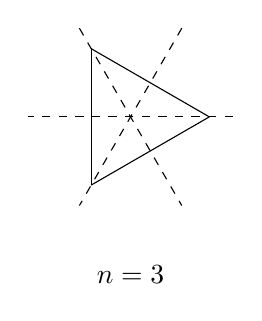
\begin{tikzpicture}[baseline=(0:0cm)]
		\foreach \x in {0,120,240}
			\draw (\x :1cm) -- (\x + 120 :1cm);
		\foreach \x in {0,60,120}
			\draw[dashed] (\x :1.3cm) -- (\x + 180 :1.3cm);
		\node at (270:2cm) {$n=3$};
	\end{tikzpicture} \qquad 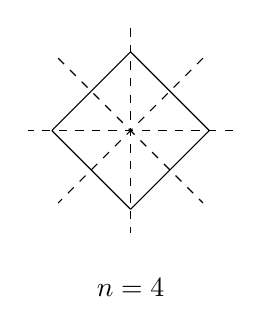
\begin{tikzpicture}[baseline=(0:0cm)]
		\foreach \x in {0,90,...,270}
			\draw (\x :1cm) -- (\x + 90 :1cm);
		\foreach \x in {0,45,...,135}
			\draw[dashed] (\x :1.3cm) -- (\x + 180 :1.3cm);
		\node at (270:2cm) {$n=4$};
	\end{tikzpicture} \qquad 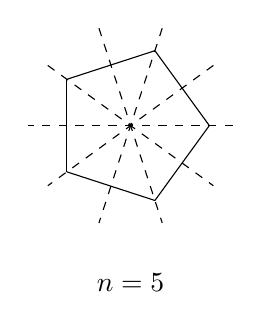
\begin{tikzpicture}[baseline=(0:0cm)]
		\foreach \x in {0,72,...,288}
			\draw (\x :1cm) -- (\x + 72 :1cm);
		\foreach \x in {0,36,...,144}
			\draw[dashed] (\x :1.3cm) -- (\x + 180 :1.3cm);
		\node at (270:2cm) {$n=5$};
	\end{tikzpicture}\end{center}
	Subgrup $N = \Z/n\Z$ bersesuaian dengan rotasi yang mempertahankan segi-$n$ beraturan itu (sudut rotasi $k + n\Z$ adalah $\frac{2\pi k}{n}$), sedangkan $n$ unsur sisanya merupakan pencerminan terhadap garis-garis putus-putus pada gambar. Sebagai contoh, $\tau$ dapat diambil sebagai pencerminan terhadap sumbu horizontal. Silakan pembaca memeriksanya.
\end{example}

Penulisan $G = NH \simeq N \rtimes H$ juga disebut dekomposisi produk semilangsung internal, sebab $NH$ dideskripsikan melalui struktur perkalian di dalam grup $G$ sendiri, sedangkan $N \rtimes H$ dapat dipandang sebagai konstruksi dari luar. Keduanya merupakan dua sudut pandang atas hal yang sama dan tidak perlu dibedakan secara kaku. Untuk produk langsung, kita juga dapat mengarakterisasi kasus dengan banyak variabel.
\begin{lemma}\label{prop:internal-direct}
	Misalkan $G_1, \ldots, G_n$ merupakan subgrup-subgrup dari grup $G$, dan andaikan bahwa
	\begin{compactitem}
		\item untuk setiap $i$, berlaku $G_i \lhd G$,
		\item untuk setiap $i$, berlaku $G_i \cap (G_1 \cdots \widehat{G_i} \cdots G_n) = \{1\}$, dengan $\widehat{\cdots}$ menyatakan bahwa suku tersebut dihilangkan,
	\end{compactitem}
	maka unsur-unsur $G_i$ dan $G_j$ saling komutatif terhadap perkalian ($i \neq j$). Dalam hal ini, $G_1 \cdots G_n$ merupakan subgrup normal dari $G$, dan
	\begin{align*}
		\prod_{i=1}^n G_i & \stackrel{\sim}{\longrightarrow} G_1 \cdots G_n \\
		(g_1, \ldots, g_n) & \longmapsto g_1 \cdots g_n.
	\end{align*}
	 Jika $G = G_1 \cdots G_n$, isomorfisme $\prod_i G_i \rightiso G$ ini disebut dekomposisi \emph{produk langsung internal} dari $G$.
\end{lemma}
\begin{proof}
	Komutativitas perkalian dan kasus $n=2$ sudah tercakup dalam Lemma \ref{prop:internal-semidirect}. Dari sini juga dapat disimpulkan bahwa, untuk setiap subbarisan $1 \leq i_1 < \cdots < i_m \leq n$, produk $G_{i_1} \cdots G_{i_m}$ tetap merupakan subgrup normal dari $G$. Penerapan Lemma \ref{prop:internal-semidirect} secara rekursif pada $n$ memberikan kasus umum.
\end{proof}

\begin{definition}[Barisan eksak] \label{def:exact-seq-group}\index{zhenghelie@barisan eksak (exact sequence)}
	Tinjau suatu barisan homomorfisme grup
	\[ \cdots \xrightarrow{f_0} G_1 \xrightarrow{f_1} G_2 \xrightarrow{f_2} \cdots \xrightarrow{f_i} G_{i+1} \to \cdots, \]
	yang panjangnya dapat berhingga ataupun tak hingga. Jika untuk setiap $i$ berlaku
	\[ \Image(f_i) = \Ker(f_{i+1}), \]
	maka barisan tersebut disebut \emph{eksak}. Kita sering menyingkat $\{1\}$ sebagai $1$, atau menuliskannya sebagai $0$ dalam notasi aditif. Sebagai contoh, untuk sebarang homomorfisme $\varphi: G \to G'$, barisan $G \to G' \to 1$ eksak jika dan hanya jika $\varphi$ surjektif, barisan $1 \to G \to G'$ eksak jika dan hanya jika $\varphi$ injektif, dan kita selalu mempunyai barisan eksak
	\[ 1 \to \Ker(\varphi) \to G \xrightarrow{\varphi} \Image(\varphi)  \to 1 \]
	dengan $\Ker(\varphi) \to G$ sebagai pemetaan inklusi natural.
\end{definition}
Barisan eksak sering digunakan bersama diagram komutatif (lihat \S\ref{sec:cat-and-morphism}). Kegunaannya baru akan tampak sepenuhnya dalam aljabar homologis.

Barisan eksak berbentuk
\[ 1 \to N \to G \xrightarrow{p} H \to 1 \]
disebut \emph{ekstensi grup}. Jika terdapat diagram komutatif homomorfisme grup\index{qunkuozhang@ekstensi grup (group extension)}
\[\begin{tikzcd}
	1 \arrow[r] & N \arrow[r] \arrow[equal, d] & G \arrow[r, "p"] \arrow[d, "\varphi"] & H \arrow[equal, d] \arrow[r] & 1 \\
	1 \arrow[r] & N \arrow[r] & G' \arrow[r, "{p'}"'] & H \arrow[r] & 1
\end{tikzcd}\]
dengan kedua baris merupakan ekstensi grup, maka $\varphi$ disebut suatu ekuivalensi ekstensi grup. Mudah diperiksa bahwa $\varphi$ pasti merupakan isomorfisme. Untuk $H$ dan $N$ yang diberikan, klasifikasi ekstensi grup hingga ekuivalensi merupakan masalah yang sesekali dijumpai dalam aljabar.

Untuk ekstensi grup $1 \to N \to G \xrightarrow{p} H \to 1$, suatu homomorfisme $s: H \to G$ yang memenuhi $p s = \identity_H$ disebut \emph{pemecahan} dari ekstensi tersebut. Dari sini dapat dibangun hubungan antara produk semilangsung dan ekstensi terpecah, sebagai berikut.
\begin{enumerate}
	\item Misalkan $G = N \rtimes_\alpha H$ suatu produk semilangsung. Maka terdapat ekstensi grup terpecah
		\[ \begin{tikzcd}
			1 \arrow[r] & N \arrow[r] & G \arrow[r, "p"] & H \arrow[bend left=30, l, "s"] \arrow[r] & 1
		\end{tikzcd} \]
		dengan $p: G \to H$ homomorfisme proyeksi $(n, h) \mapsto h$, sedangkan $s: H \hookrightarrow G$ homomorfisme inklusi $s(h) = (1,h)$.
	\item Sebaliknya, jika diberikan ekstensi grup di atas beserta pemecahannya $s$, definisikan $\alpha: H \to \Aut(N)$ melalui pembatasan automorfisme adjoin, $\alpha(h) = \Ad(s(h))|_N$. Maka terdapat ekuivalensi ekstensi grup
		\[ \begin{tikzcd}
			1 \arrow[r] & N \arrow[r] \arrow[equal, d] & N \rtimes_\alpha H \arrow[r] \arrow[d, "\varphi"] & H \arrow[equal, d] \arrow[r] & 1 \\
			1 \arrow[r] & N \arrow[r] & G \arrow[r] & H \arrow[r] & 1
		\end{tikzcd} \]
		dengan $\varphi(n, h) := n s(h)$. Silakan pembaca memeriksa bahwa $\varphi$ memang merupakan homomorfisme grup yang injektif.
\end{enumerate}
\section{Aksi Grup dan Prinsip Pencacahan}\label{sec:group-action}
Baik dari sudut penerapan nyata maupun perkembangan historis, suatu grup abstrak sering dideskripsikan melalui aksinya pada sebuah himpunan, sedangkan pengkajian berbagai aksi grup merupakan sarana penting untuk meneliti sifat-sifat grup. Tujuan pertama bagian ini ialah memperjelas konsep-konsep dasar aksi grup.

\begin{definition}[Aksi monoid]\label{def:monoid-action} \index{qunzuoyong@aksi grup (group action)}
	Misalkan $X$ suatu himpunan dan $M$ suatu monoid. Suatu aksi $M$ pada $X$ didefinisikan sebagai pemetaan
	\[ a: M \times X \to X, \]
	yang disebut pemetaan aksi dan harus memenuhi sifat-sifat berikut:
	\begin{compactenum}[(i)]
		\item untuk setiap $g,g' \in M$ dan $x \in X$, berlaku $a(g', a(g, x)) = a(g'g, x)$ (hukum asosiatif),
		\item untuk setiap $x \in X$, berlaku $a(1, x)=x$.
	\end{compactenum}
	Himpunan yang dilengkapi aksi $M$ disebut himpunan-$M$. Aksi yang untuk setiap $m,x$ memenuhi $a(m,x)=x$ disebut \emph{aksi trivial}. Suatu pemetaan di antara himpunan-$M$, yaitu $f: X \to Y$,
	\[ f(a(m, x)) = a(m, f(x)), \quad m \in M, x \in X \]
	disebut pemetaan $M$-\emph{ekuivarian} jika memenuhi persamaan tersebut. Jika pemetaan-pemetaan ekuivarian
	\begin{tikzcd}
		X \arrow[yshift=0.5ex, r, "f"] & Y \arrow[yshift=-0.5ex, l, "g"]
	\end{tikzcd}
	memenuhi $fg = \identity_Y$, $gf = \identity_X$, maka $f, g$ disebut isomorfisme yang saling invers. Dengan demikian, kita dapat mendefinisikan konsep isomorfisme antara himpunan-$M$.
\end{definition}

\begin{remark}
	Singkatnya, untuk $M$ yang diberikan, semua himpunan-$M$ beserta pemetaan ekuivarian membentuk suatu kategori $M\dcate{Set}$. Secara ketat, ukuran himpunan-$M$ $X$ juga harus dibatasi: kita perlu mengandaikan bahwa $M$ dan $X$ termasuk dalam semesta yang sama dan telah dipilih, yaitu $\mathcal{U}$; lihat Definisi \ref{def:U-cat} beserta pembahasan terkait.
\end{remark}

% Dalam bahasa Contoh \ref{eg:symmetric-group}, suatu aksi $M$ pada $X$ ekuivalen dengan pemberian homomorfisme $M \to \Aut(X)$: setiap $m \in M$ dipetakan ke bijeksi $\left[ x \mapsto a(m,x) \right] \in \Aut(X)$.

Menurut kebiasaan, pemetaan aksi yang melekat pada suatu himpunan-$M$ tidak dituliskan, dan $a(m, x)$ ditulis sebagai $m \cdot x$ atau $mx$. Syarat bagi pemetaan aksi dan ekuivariansinya lalu mengambil bentuk alami
\begin{gather*}
	m'(mx) = (m'm)x, \\
	1 \cdot x = x, \\
	f(mx) = mf(x),
\end{gather*}
dengan $ m, m' \in M, x \in X$. Aksi yang didefinisikan demikian disebut aksi kiri $M$, sebab dinyatakan melalui perkalian kiri oleh $M$. Dengan cara yang sama, kita dapat mendefinisikan aksi kanan $M$, yakni $(x, m) \mapsto xm$. Definisi di atas dapat ditulis ulang butir demi butir, misalnya $(xm)m' = x(mm')$, dan seterusnya. Cara yang sekaligus menangani semuanya ialah menggunakan dualitas: aksi kanan $M$ tidak lain merupakan aksi kiri $M^\text{op}$. Setiap pernyataan dalam bagian ini mengenai aksi kiri memiliki versi kanan yang bersesuaian dan tidak akan diulangi.

\begin{example}
	Untuk setiap himpunan $X$, grup simetris $\mathfrak{S}_X$ beraksi secara alami pada $X$: $a: (\sigma, x) \mapsto \sigma(x)$. Demikian pula, monoid matriks real $n \times n$, yaitu $M_n(\R)$, beraksi pada $\R^n$: dengan memandang unsur $\R^n$ sebagai matriks kolom berukuran $n \times 1$, aksi $(A, x) \mapsto A x$ tidak lain adalah perkalian matriks.
\end{example}

\begin{example}
	Jika grup $G$ beraksi dari kiri pada $X$ dan $Y$ merupakan sebarang himpunan, maka terdapat aksi kiri alami $G$ pada $\{f: \text{pemetaan}\; X \to Y \}$ yang diberikan oleh $a(g,f) = \left[ x \mapsto f(g^{-1}x) \right]$; jika $G$ beraksi dari kanan pada $X$, aksi kiri yang bersesuaian diberikan oleh $[x \mapsto f(xg)]$. Verifikasilah rinciannya.
\end{example}

\begin{example}
	Pembahasan berikut dapat dibandingkan dengan \cite[Contoh 7.2.4]{Zh2}. Misalkan $n \geq 1$, dan misalkan ruang $C_\infty(\R^n)$ merupakan penutupan ruang fungsi turun cepat $\mathscr{S}(\R^n)$ (lihat \cite[Contoh 3.2.7]{Zh1}) di dalam $L^\infty(\R^n)$. Definisikan aksi monoid $(\R_{\geq 0}, +)$ pada $C_\infty(\R^n)$ sebagai berikut:
	\[ a(t, u) =
		\begin{cases}
			G_t \ast u, & t > 0, \\
			u, & t=0,
		\end{cases}\]
	dengan $\ast$ menyatakan konvolusi dan $G_t$ merupakan fungsi kernel panas yang dikenal pada $\R^n$,
	\[ G_t(x) := (4\pi t)^{-\frac{n}{2}} e^{-\|x\|^2 /4t}, \quad x \in \R^n. \]
	Menurut teori persamaan panas, $v(t, \cdot) := a(t, u)$ memenuhi masalah nilai awal $\frac{\partial v}{\partial t} = \Delta v$, $v(0, \cdot) = u(\cdot)$; karena itu, $a$ memang memberikan suatu aksi monoid. Dalam analisis fungsional, aksi ini disebut semigrup operator. Karena hantaran panas menghaluskan singularitas fungsi, aksi ini tidak dapat diperluas menjadi aksi grup $(\R, +)$.
\end{example}

\begin{definition}\index{guidao@orbit (orbit)}\index{wendinghuazi@stabilisator (stabilizer)}\index[sym1]{Stab@$\Stab$}
	Misalkan monoid $M$ beraksi pada $X$. Definisikan
	\begin{compactitem}
		\item himpunan \emph{titik tetap} $X^M := \{x \in X: \forall m \in M, \; mx=x \}$;
		\item untuk $x \in X$, \emph{orbit} $Mx := \{mx : m \in M \}$, yang setiap unsurnya disebut wakil orbit tersebut; orbit $Mx$ merupakan subhimpunan dari $X$ yang stabil di bawah $M$;
		\item dengan notasi di atas, \emph{stabilisatornya} didefinisikan sebagai submonoid dari $M$, yaitu $\Stab_M(x) := \{m \in M : mx=x\}$.
	\end{compactitem}
\end{definition}

Aksi yang paling sering digunakan tetaplah aksi grup. Bagi suatu grup $G$, blok pembangun dasar bagi aksi adalah ruang koset berbentuk $G/H$, dengan pemetaan aksi $(g, xH) \mapsto gxH$. Hasil berikut menjelaskan cara menguraikan himpunan-$G$ umum sebagai gabungan saling lepas ruang-ruang koset. Inilah pula titik awal prinsip pencacahan.

\begin{lemma}\label{prop:orbit-decomp}
	Misalkan grup $G$ beraksi pada $X$. Maka:
	\begin{compactenum}[(i)]
		\item terdapat dekomposisi orbit $X = \bigsqcup_x Gx$, dengan memilih satu wakil $x$ dari setiap orbit;
		\item untuk setiap $x \in X$, pemetaan
			\begin{align*}
				G/\Stab_G(x) & \longrightarrow Gx \\
				g \cdot \Stab_G(x) & \longmapsto gx
			\end{align*}
			merupakan isomorfisme antara himpunan-$G$;
		\item khususnya, kita mempunyai persamaan kardinal (lihat \eqref{eqn:cardinal-infinite-sum})
			\[ |X| = \sum_x \left( G: \Stab_G(x) \right); \]
		\item untuk setiap $x \in X$ dan $g \in G$, berlaku
			\[ \Stab_G(gx) = g \Stab_G(x) g^{-1}. \]
	\end{compactenum}
\end{lemma}
\begin{proof}
	Pertama, kita buktikan bahwa jika dua orbit $Gx, Gy$ beririsan, maka $Gx=Gy$. Memang, jika $gx=g'y$, maka $x = g^{-1}g' y \in Gy$, sehingga $Gx \subset Gy$; berdasarkan simetri, diperoleh $Gx=Gy$. Karena $\forall x, \; x = 1\cdot x \in Gx$, dekomposisi orbit segera diperoleh. Pernyataan mengenai pemetaan $G/\Stab_G(x) \to Gx$ merupakan akibat langsung dari definisi stabilisator. Bersama dekomposisi orbit, hal ini menghasilkan persamaan kardinal. Persamaan terakhir dapat diverifikasi langsung dari definisi.
\end{proof}

Dengan demikian, sifat ``$x,y$ berada dalam orbit yang sama'' memberikan suatu relasi ekuivalensi pada $X$. Himpunan hasil bagi yang bersesuaian, atau ruang orbit, dinotasikan dengan $G \backslash X$; bagi aksi kanan, ruang orbit secara alami dinotasikan dengan $X/G$. Perhatikan bahwa memberikan aksi $G$ pada $X$ ekuivalen dengan memberikan homomorfisme $G \to \mathfrak{S}_X$ yang memetakan $g$ ke $[x \mapsto gx]$.
\begin{definition}
	Misalkan $G$ suatu grup dan $X$ suatu himpunan-$G$. Aksi $G$ pada $X$ disebut \index{qunzuoyong!setia (faithful)}\index{qunzuoyong!transitif (transitive)}
	\begin{compactitem}
		\item setia, jika homomorfisme $G \to \mathfrak{S}_X$ yang bersesuaian merupakan injeksi; ini ekuivalen dengan $\bigcap_{x \in X} \Stab_G(x) = \{1\}$;
		\item bebas atau semireguler, jika untuk setiap $x \in X$ berlaku $\Stab_G(x) = \{1\}$;
		\item transitif, jika $X$ hanya mempunyai satu orbit; ini ekuivalen dengan mensyaratkan bahwa $X$ tidak kosong dan, untuk setiap $x, y \in X$, terdapat $g \in G$ sedemikian sehingga $gx=y$;
		\item lebih umum, jika untuk setiap $1 \leq m \leq n$, grup $G$ beraksi secara transitif pada $\{ (x_1, \ldots, x_m) \in X^m: \text{unsur-unsur berbeda} \}$, maka aksi $G$ pada $X$ disebut $n$-transitif.
	\end{compactitem}

	Himpunan-$G$ yang transitif juga disebut \emph{ruang homogen}-$G$, sedangkan ruang homogen-$G$ yang bebas disebut \emph{ruang homogen utama}-$G$ atau \emph{torsor}.\index{qixingkongjian@ruang homogen (homogeneous space)}\index{naozi@torsor (torsor)}
\end{definition}
Sebagai akibat dari Lema \ref{prop:orbit-decomp}, hingga isomorfisme, ruang koset $G/H$ mencakup semua ruang homogen.

Istilah-istilah ini jelas berasal dari geometri, yang untuk itu struktur manifold dan ruang dasar perlu diperkenalkan. Namun, bagian ini hanya membahas himpunan, dan penerapan utamanya adalah masalah pencacahan himpunan; lihat \S\ref{sec:Sylow}. Untuk sementara, mari kita tinjau beberapa contoh umum.

\begin{example}[Aksi translasi dan koset]
	Misalkan $G$ suatu grup dan $H$ subgrupnya. Aksi kiri $H$ pada $G$ yang diberikan oleh $(h, g) \mapsto hg$ disebut aksi translasi kiri. Jelas bahwa
	\begin{inparaenum}[(i)]
		\item orbit-orbit yang bersesuaian tidak lain adalah koset $Hg$ ($g \in G$),
		\item ruang orbitnya tidak lain adalah ruang koset $H \backslash G$,
		\item aksi ini bebas, dan transitif jika dan hanya jika $H=G$.
	\end{inparaenum}
	Pernyataan yang sama berlaku bagi aksi translasi kanan $H$ pada $G$, yaitu $(g,h) \mapsto gh$; ruang orbit yang bersesuaian tidak lain adalah $G/H$.

	Sekarang misalkan $H, K$ subgrup-subgrup dari $G$. Koset ganda mempunyai penafsiran serupa: tinjau aksi kiri $H \times K^\text{op}$ pada $G$,
	\[ ((h, k), g) \mapsto hgk, \quad (h, k) \in H \times K^\text{op}, \; g \in G. \]
	Orbit yang bersesuaian tepat merupakan koset-koset ganda $HgK$ ($g \in G$), sedangkan ruang orbitnya diidentifikasi dengan $H \backslash G/K$. Namun, sifat-sifat lain aksi ini jauh lebih rumit daripada dalam kasus koset kiri atau koset kanan.
\end{example}

\begin{example}[Aksi konjugasi]\label{eg:conj-action} \index{gonge@konjugasi (conjugation)}
	Tetap misalkan $G$ suatu grup. Homomorfisme adjoin $\Ad: G \to \Aut(G)$ memberikan aksi $G$ yang disebut \emph{aksi konjugasi} pada dirinya sendiri, yakni $G \times G \to G$ (di sini kita meninjau aksi kiri). Setelah definisinya diuraikan, aksi ini tidak lain adalah
	\[ (g, x) \longmapsto {}^g x := gxg^{-1}. \]
	Orbit di bawah aksi konjugasi disebut \emph{kelas konjugasi} dalam $G$.

	Lebih umum, untuk sebarang subhimpunan $E \subset G$, kita telah mendefinisikan subgrup $N_G(E)$; aksinya pada $E$ juga disebut konjugasi. Jika dua subhimpunan $E, E'$ memenuhi $\exists g \in G, \; E' = gEg^{-1}$, maka $E$ dan $E'$ disebut saling konjugat.

	Perilaku aksi konjugasi pada grup nonkomutatif umumnya cukup rumit. Untuk $x \in G$, subgrup stabilisatornya tepat merupakan sentralisator $Z_G(x)$, sedangkan himpunan titik tetapnya adalah pusat $Z_G$. Menganalisis aksi konjugasi $G$ merupakan langkah yang tak terelakkan untuk memahami struktur grup tersebut.
\end{example}

Torsor merupakan jenis himpunan-$G$ yang sangat umum dijumpai. Bahasa ini baru menunjukkan kekuatannya apabila dilengkapi latar belakang geometri yang sesuai; lihat \S\ref{sec:group-in-cat}. Berikut hanya diperkenalkan contoh yang paling dasar.
\begin{example}
	Misalkan $G_1$, $G_2$ grup, dan tetapkan
	\[ \Isom(G_1, G_2) := \{ \text{ isomorfisme } \; \varphi: G_1 \to G_2 \}. \]
	Jika $\Isom(G_1, G_2)$ tidak kosong, terdapat aksi kiri $\Aut(G_2)$ padanya, yakni $(g, \varphi) \mapsto g \circ \varphi$, dengan $g \in \Aut(G_2)$. Aksi ini menjadikan $\Isom(G_1, G_2)$ suatu torsor-$\Aut(G_2)$. Walaupun yang ditinjau di sini hanya isomorfisme grup, konstruksi serupa sebenarnya dapat dilakukan dalam sebarang kategori; lihat \S\ref{sec:cat-and-morphism}.

	Kita tentu tidak perlu membatasi diri pada aksi kiri: $\Aut(G_1)$ juga beraksi dari kanan pada $\Isom(G_1, G_2)$ melalui komposisi pemetaan. Aksi di kedua sisi ini memenuhi $(g \circ \varphi) \circ g' = g \circ (\varphi \circ g')$, sehingga dapat digabungkan menjadi aksi $\Aut(G_1)^{\text{op}} \times \Aut(G_2)$. Baik dilihat dari kiri maupun kanan, $\Isom(G_1, G_2)$ merupakan torsor. Struktur semacam ini disebut bitorsor.
\end{example}

Definisi asli torsor agak tidak langsung. Namun, terdapat karakterisasi ringkas berikut, yang akan sangat berguna dalam kerangka teori kategori; lihat \S\ref{sec:group-in-cat}.

\begin{lemma}\label{prop:torsor-criterion}
	Misalkan $X$ suatu himpunan-$G$ yang tidak kosong. Maka $X$ merupakan torsor jika dan hanya jika pemetaan
	\begin{align*}
		\Phi: G \times X & \longrightarrow X \times X \\
		(g, x) &  \longmapsto (x, gx)
	\end{align*}
	merupakan bijeksi.
\end{lemma}
\begin{proof}
	Menurut definisi, $\Phi^{-1}(x,y) = \{g \in G: gx=y\} \times \{x\}$. Karena itu, pemetaan $\Phi$ injektif jika dan hanya jika $X$ bebas, dan surjektif jika dan hanya jika $X$ transitif.
\end{proof}
\section{Sylow 定理}\label{sec:Sylow}
首先引入 $p$-群的概念.

\begin{definition}\label{def:p-group}\index{$p$-群}
	设 $p$ 为素数. 满足 $|G|=p^m$, $m \in \Z_{\geq 0}$ 的群 $G$ 称为 $p$-群.
\end{definition}
应用命题 \ref{prop:Lagrange}, 易见 $p$-群的子群和商群仍是 $p$-群.

\begin{proposition}\label{prop:counting-localization}
	设 $G$ 为非平凡 $p$-群, 则任意有限 $G$-集 $X$ 皆满足
	\[ |X| \equiv \left\lvert X^G \right\rvert \mod p. \]
\end{proposition}
\begin{proof}
	对任意 $x \in X$, 命题 \ref{prop:Lagrange} 蕴涵 $(G: \Stab_G(x))$ 是 $p$ 的幂. 故有
	\[ [ x \notin X^G] \iff [ \Stab_G(x) \neq G ] \iff (G: \Stab_G(x)) \equiv 0 \bmod p . \]
	套入引理 \ref{prop:orbit-decomp} 即得所求.
\end{proof}

\begin{corollary}\label{prop:p-group-center}
	设 $G$ 为非平凡的 $p$-群, 则 $Z_G \neq \{1\}$.
\end{corollary}
\begin{proof}
	考虑 $G$ 的共轭作用 (例 \ref{eg:conj-action}). 由命题 \ref{prop:counting-localization} 得到
	\[ 0 \equiv |G| \equiv |Z_G| \mod p , \]
	故 $|Z_G| > 1$.
\end{proof}

此式可用以递归地研究 $p$-群的结构, 兹举一例.
\begin{corollary}
	设 $G$ 为 $p$-群而 $H \subsetneq G$ 为真子群, 则 $H \subsetneq N_G(H)$. 特别地, $(G:H)=p$ 蕴涵 $H \lhd G$.
\end{corollary}
\begin{proof}
	已知 $Z_G$ 非平凡, 显然 $Z_G \subset N_G(H)$. 若 $Z_G \not\subset H$, 则 $H \subsetneq Z_G H \subset N_G(H)$. 因此不妨假设 $Z_G \subset H$. 现在对 $|G|$ 递归论证: 定义 $\bar{G} := G/Z_G$, $\bar{H} := H/Z_G$, 可假设
	\[ \bar{H} \subsetneq N_{\bar{G}}(\bar{H}). \]
	容易看出 $N_G(H)/Z_G = N_{\bar{G}}(\bar{H})$. 应用命题 \ref{prop:2nd-homomorphism} 即得 $H \subsetneq N_G(H)$.
\end{proof}

另一个直接而重要的推论如下. 先回忆我们在 \S\ref{sec:group-and-monoid} 定义的元素 $x \in G$ 的阶 $\text{ord}(x)$.
\begin{corollary}[Cauchy 定理]\label{prop:group-Cauchy}
	设 $G$ 为有限群, 素数 $p$ 整除 $|G|$, 则存在 $x \in G$ 使得 $\ord(x)=p$.
\end{corollary}
\begin{proof}
	定义集合
	\[ X_p := \{(g_i)_{1 \leq i \leq p} \in G^p : g_1 \cdots g_p = 1 \}. \]
	不妨将下标 $1 \leq i \leq p$ 看成 $\Z/p\Z$ 里的元素. 如此一来循环群 $\Z/p\Z$ 就作用在 $X_p$ 上: 陪集 $m + p\Z$ 的作用是平移下标
	\[ (g_i)_{i \in \Z/p\Z} \longmapsto (g_{i+m})_{i \in \Z/p\Z}. \]
	须证明此作用不逸出 $X_p$, 仅须检查 $m=1$ 的情形: 对等式 $g_1 \cdots g_p = 1$ 左乘以 $g_1^{-1}$, 右乘以 $g_1$ 即是. 由此导出 $(X_p)^{\Z/p\Z} = \{(x, \ldots, x) : x^p = 1 \}$. 注意到 $x^p=1$ 且 $x \neq 1$ 等价于 $\ord(x)=p$ (参看例 \ref{eg:cyclic-group}).

	由于 $g_p = (g_1 \cdots g_{p-1})^{-1}$, 投影映射 $X_p \to G^{p-1}$, $(g_i)_{1 \leq i \leq p} \mapsto (g_i)_{1 \leq i < p}$ 是双射, 故
	\[ |X_p| = |G|^{p-1} \equiv 0 \mod p. \]
	另一方面, 命题 \ref{prop:counting-localization} 给出
	\[ |X_p| \equiv \left\lvert(X_p)^{\Z/p\Z}\right\rvert = 1 + \left\lvert \{x \in G : \ord(x)=p \} \right\rvert \mod p , \]
	故 $\{x \in G : \ord(x)=p \}$ 非空.
\end{proof}

\begin{convention}
	设 $p$ 为素数, $n \in \Z_{\geq 1}$, 若 $p^a \mid n$ 而且 $p^{a+1} \nmid n$, 则写作 $p^a \| n$.
\end{convention}

\begin{definition}\index{Sylow $p$-子群}
	设 $G$ 为 $n$ 阶有限群, $p$ 为素数. 设 $p^m \| n$, 满足 $|H| = p^m$ 的子群 $H$ 称为 $G$ 的 Sylow $p$-子群.
\end{definition}
这意谓 $p$-子群 $H$ 在 Lagrange 定理的约束下达到最大可能阶数. 此定义显然仅在 $p \mid n$ 时才有实质意涵.

\begin{lemma}\label{prop:Wielandt-lemma}
	设 $p$ 为素数. 对任意非负整数 $b \leq a$, $a \neq 0$ 和 $m$, 二项式系数满足同余式
	\[ \binom{p^m a}{p^m b} \equiv \binom{a}{b} \mod p. \]
\end{lemma}
\begin{proof}
	考虑以符号 $T$ 为变元的整系数多项式. 由于 $0 < c < p \implies p \mid \binom{p}{c}$, 故
	\[ (T+1)^{pa} = \left( T^p + p(\cdots) + 1 \right)^a \equiv (T^p + 1)^a \mod p. \]
	即: 两边逐系数模 $p$ 同余. 两侧以二项式定理展开, 比较 $T^{pb}$ 的系数即得 $m=1$ 的情形. 迭代 $m$ 次遂得一般情形.
\end{proof}

\begin{theorem}[Sylow 第一定理]
	对任意素数 $p$, 任意有限群 $G$ 含有 Sylow $p$-子群.
\end{theorem}
下面论证供鉴赏之用, 另有它证如 \cite[Theorem 6.2]{Lang02}.
\begin{proof}[H.\ Wielandt]
	置 $n := |G|$, 不妨假设 $p^m \| n$, $m \geq 1$. 定义
	\[ Y := \left\{ \text{ 子集 } \; E \subset G : |E|=p^m \right\}. \]
	由引理 \ref{prop:Wielandt-lemma} 知
	\[ |Y| = \binom{n}{p^m} \equiv \binom{p^{-m} n}{1} = p^{-m} n \not\equiv 0 \mod p . \]

	群 $G$ 以左平移 $(g, E) \mapsto gE$ 作用于 $Y$. 由引理 \ref{prop:orbit-decomp} 和以上同余式知存在 $E \in Y$ 使得 $p \nmid (G: \Stab_G(E))$, 我们断言 $H := \Stab_G(E)$ 是 Sylow $p$-子群. 首先注意到 $p \nmid \frac{|G|}{|H|}$ 故 $p^m$ 整除 $|H|$. 任取 $g \in E$, 由稳定化子的性质知 $Hg  \subset E$; 配合 $|H|=|Hg|$ 遂得到 $|H| \leq  |E| = p^m$, 故 $|H|=p^m$. 明所欲证.
\end{proof}

\begin{lemma}
	设 $p$ 为素数, 而$P$ 是 $G$ 的 Sylow $p$-子群. 若 $G$ 的 $p$-子群 $H$ 满足 $H \subset N_G(P)$, 则 $H \subset P$.
\end{lemma}
\begin{proof}
	对群 $HP$ 应用命题 \ref{prop:3rd-homomorphism} 可得群同构 $HP/P \simeq H/H \cap P$, 故 $HP$ 仍是 $p$-群. 又因为 $P \subset HP \subset G$ 而 $P$ 是 Sylow $p$-子群, 必有 $HP=P$, 而这又等价于 $H \subset P$.
\end{proof}

\begin{theorem}[Sylow 第二定理]
	令 $G$ 为有限群, $p$ 为素数. 则
	\begin{compactenum}[(i)]
		\item 任意 $p$-子群 $H \subset G$ 皆包含于某个 Sylow $p$-子群;
		\item $G$ 的任两个 Sylow $p$-子群 $P, P'$ 皆共轭;
	\end{compactenum}
	特别地, $G$ 中存在正规的 Sylow $p$-子群 当且仅当 $G$ 有唯一的 Sylow $p$-子群.
\end{theorem}
\begin{proof}
	选定 Sylow $p$-子群 $P \subset G$, 并考虑它在 $G$ 的共轭作用下的轨道
	\[ X := \left\{ gPg^{-1} : g \in G \right\} \]
	任意 $Q \in X$ 都是 $G$ 的 Sylow $p$-子群, 而且其稳定化子群是 $N_G(Q)$. 我们有 $G$-集的同构
	\begin{align*}
		G/N_G(P) & \stackrel{\sim}{\longrightarrow} X \\
		g N_G(P) & \longmapsto gPg^{-1}.
	\end{align*}

	由于 $P \subset N_G(P)$, 我们有 $|X| \not\equiv 0 \mod p$. 现假设 $H \subset G$ 为 $p$-子群, 那么 $H$ 也共轭作用于 $X$ 上. 应用命题 \ref{prop:counting-localization} 得 $X^H$ 非空. 取 $Q \in X^H$, 从定义知 $H \subset N_G(Q)$, 上述引理遂保证 $H \subset Q$, 这就证明了第一个断言. 若进一步要求 $H$ 为  Sylow $p$-子群, 则必有 $H = Q$. 由于 $X$ 中元素相互共轭, 第二个断言随之得证.
\end{proof}

\begin{theorem}[Sylow 第三定理]
	承上, $G$ 中 Sylow $p$-子群的个数 $\equiv 1 \mod p$.
\end{theorem}
\begin{proof}
	沿用上个证明的框架, 选定 Sylow $p$-子群 $P$ 并取 $H = P$, 以上业已证明了 $X^P$ 中的元素必为包含 $P$ 的 $p$-子群, 故 $X^P = \{P\}$. 套回命题 \ref{prop:counting-localization} 遂得 $|X| \equiv \left\lvert X^P \right\rvert = 1 \mod p$.
\end{proof}

\begin{proposition}
	 对每个素数 $p$, 有限群 $G$ 的每个 Sylow $p$-子群皆正规的充分必要条件是 $G = \prod_{p \mid\; |G|} H_p$, 其中 $H_p$ 是 $p$-子群.
\end{proposition}
\begin{proof}
	设 $p_1 < \cdots < p_r$ 为素数. 若 $G$ 同构于直积 $\prod_{i=1}^r H_{p_i}$, 其中 $|H_{p_i}| = p_i^{a_i}$ ($a_i \in \Z_{\geq 1}$), 那么 $H_{p_i}$ 自然地嵌入为 $G$ 的正规 Sylow $p_i$-子群, 而 $|G| = \prod_{i=1}^r p_i^{a_i}$.
	
	反过来设 $|G| = p_1^{a_1} \cdots p_r^{a_r}$, 而且对每个 $1 \leq i \leq r$ 皆有正规 Sylow $p_i$-子群 $H_{p_i}$. 它们的阶数两两互素, 运用命题 \ref{prop:Lagrange} 可以在 $G$ 中验证 $H_{p_i} \cap \prod_{j \neq i} H_{p_j} = \{1\}$. 于是引理 \ref{prop:internal-direct} 的条件成立, 得到同构 $\prod_{i=1}^r H_{p_i} \rightiso H_{p_1} \cdots H_{p_r} \subset G$. 比较阶数可知 $H_{p_1} \cdots H_{p_r} = G$.
\end{proof}

\section{群的合成列}\label{sec:composition-series-grp}
将一个群设法拆解为较小的构件是群论的常见手法, 合成列是其中一例.

\begin{definition}[正规列]\label{def:normal-series}\index{zhengguilie@正规列 (normal series)}
	群 $G$ 的递降子群链
	\[ G = G_0 \supset G_1 \supset \cdots \supset G_n = \{1\} \]
	如满足 $\forall 0 \leq i < n,\;  G_{i+1} \lhd G_i$, 则称之为\emph{正规列}, 而群族
	\[ G_i/G_{i+1}, \quad i=0, \ldots, n-1 \]
	称为该列的\emph{子商}. 正规列的\emph{加细}是透过形如 \index{zishang@子商 (subquotient)}
	\[ \left[ \cdots \supset G_i \supset G_{i+1} \supset \cdots \right] \leadsto \left[ \cdots \supset G_i \supset G' \supset G_{i+1} \supset \cdots \right] \]
	的反复插项得到的新列. 插入 $G' = G_i$ 或 $G_{i+1}$ 得到的加细是平凡的; 反之则称为\emph{真加细}.
\end{definition}

下节将考虑一种特殊的正规列, 在此一并定义.
\begin{definition}[中心列]\label{def:central-series}\index{zhongxinlie@中心列 (central series)}
	群 $G$ 的正规列 $G = G_0 \supset G_1 \supset \cdots$ 如对每个 $i$ 都满足
	\begin{gather*}
		G_i \lhd G, \\
		G_i/G_{i+1} \subset Z_{G/G_{i+1}},
	\end{gather*}
	则称为\emph{中心列}.
\end{definition}

\begin{definition}[合成列]\label{def:composition-series}\index{hechenglie@合成列 (composition series)}
	若群 $G$ 的正规列 $G = G_0 \supset G_1 \supset \cdots$ 满足 $G_{i+1} \subsetneq G_i$, 而且子商皆为单群, 则称之为\emph{合成列}.
\end{definition}
细观单群定义可见合成列正是无冗余项, 而且无法再(真)加细的列. 有限群总有合成列, 一般的群则未必.

\begin{lemma}[Zassenhaus 引理]\label{prop:Zassenhaus}
	固定群 $G$, 考虑子群 $U, V$ 及各自的正规子群 $u \lhd U$, $v \lhd V$. 则有
	\begin{gather*}
		u(U \cap v) \lhd u(U \cap V), \\
		(u \cap V) v \lhd (U \cap V)v,
	\end{gather*}
	其中各项在注记 \ref{rem:HN} 的意义下都是子群, 而且有自然的同构
	\[ \dfrac{u (U \cap V)}{u (U \cap v)} \simeq \dfrac{(U \cap V)v}{(u \cap V)v}. \]
\end{lemma}
\begin{proof}
	我们将表解各子群之间的关系, 图例如下:
	\[ \begin{tikzcd}
		G \arrow[dash, d] \\ H: \text{子群}
	\end{tikzcd} \quad
	\begin{tikzcd}
		G \arrow[dash, d, "\triangledown" description] \\ N: \text{正规子群}
	\end{tikzcd} \quad
	\begin{tikzcd}[column sep=tiny]
		A \arrow[dash, rd] & & B \arrow[dash, ld] \\
		& A \cap B &
	\end{tikzcd} \quad
	\begin{tikzcd}[column sep=tiny]
		{}& HN \arrow[dash, ld] \arrow[dash, rd, "\triangledown" description] & \\
		H & & N
	\end{tikzcd}\]
	其中 $H \subset N_G(N)$. 现断言有以下图表:
	\[ \begin{tikzcd}[column sep=tiny]
		{} & U \arrow[dash, d] & & V \arrow[dash, d] & \\
		& u(U \cap V) \arrow[dash, dd, "\triangledown" description] \arrow[dash, rd] & & (U \cap V)v \arrow[dash, dd, "\triangledown" description] \arrow[dash, ld] & \\
		& & U \cap V \arrow[dash, dd, "\triangledown" description] & & \\
		& u(U \cap v) \arrow[dash, ld] \arrow[dash, rd] & & (u \cap V)v \arrow[dash, ld] \arrow[dash, rd] & \\
		u \arrow[dash, rd] & & (u \cap V)(U \cap v) \arrow[dash, ld] \arrow[dash, rd] & & v \arrow[dash, ld] \\
		& u \cap V & & U \cap v &
	\end{tikzcd} \]
	首先留意有性质 $U \cap V \subset N_G(u) \cap N_G(v)$ 等等, 图中的积 $u(U \cap V)$ 等因而是子群. 图例第一条 (即: 子群在下) 显然成立. 又可逐一验证
	\begin{align*}
		u(U \cap v) \cap (U \cap V) & = (u \cap V)(U \cap v) = (U \cap V) \cap (u \cap V)v, \\
		u \cap (u \cap V)(U \cap v) & = u \cap V, \\
		(u \cap V)(U \cap v) \cap v & = U \cap v.
	\end{align*}
	故图例第三条 (子群交) 也成立. 同理可验证图例第四条 (子群积). 至于第二条 (正规子群), 从 $v \lhd V$ 可导出 $U \cap v \lhd U \cap V$, 从而 $u(U \cap v) \lhd u(U \cap V)$; 同理有 $(u \cap V)v \lhd (U \cap V)v$, 取交即得 $(u \cap V)(U \cap v) \lhd U \cap V$. 至此证成断言.

	现在考虑图表中的两个平行四边形. 分别运用命题 \ref{prop:3rd-homomorphism} 可得自然同构
	\begin{equation*}\begin{tikzcd}[column sep=tiny, row sep=small]
		\dfrac{u (U \cap V)}{u(U \cap v)} \arrow[rd, "\simeq"'] &  & \dfrac{(U \cap V)v}{(u \cap V)v} \arrow[ld, "\simeq"] \\
		& \dfrac{U \cap V}{(u \cap V)(U \cap v)} &
	\end{tikzcd}\end{equation*}
	明所欲证.
\end{proof}

\begin{definition}\label{def:JH-subquotients}
	设 $G = G_0 \supset \cdots$ 为正规列, 我们视其子商 $(G_i/G_{i+1})_{i \geq 0}$ 为不计顺序, 但计入重数的集合. 如果两个正规列长度相同, 而且其子商在上述意义下相等, 则称两正规列\emph{等价}.
\end{definition}

\begin{theorem}[Schreier 加细定理]\label{prop:Schreier}
	设
	\begin{align*}
		G & = G_0 \supset \cdots \supset G_r \supset G_{r+1} = \{1\}, \\
		G & = H_0 \supset \cdots \supset H_s \supset H_{s+1} = \{1\}
	\end{align*}
	为 $G$ 的两个正规列, 则两者有等价的加细.
\end{theorem}
\begin{proof}
	对每个 $0 \leq i \leq r$, $0 \leq j \leq s$ 定义
	\begin{align*}
		G_{i,j} & := G_{i+1} (H_j \cap G_i), \\
		H_{j,i} & := (G_i \cap H_j) H_{j+1}.
	\end{align*}
	先看 $G_{i,j}$, 由 $G_{i+1} \lhd G_i$ 知其为子群. 包含关系 $G_{i, j+1} \lhd G_{i,j}$ 成立, 而且
	\[ G_{i,0} = G_{i+1} (G \cap G_i) = G_i, \quad G_{i,s+1} = G_{i+1}, \]
	遂得到 $(G_i)_{i=0}^r$ 的加细
	\[ \mathcal{G} := \left[ \cdots \supset G_i = G_{i, 0} \supset G_{i, 1} \supset \cdots G_{i, s} \supset G_{i, s+1}= G_{i+1} \supset \cdots \right] . \]
	同理可见 $H_{j, i}$ 给出 $(H_j)_{j=0}^s$ 的加细, 记为 $\mathcal{H}$. 在引理 \ref{prop:Zassenhaus} 中取 $u := G_{i+1}$, $U := G_i$ 和 $v := H_{j+1}$, $V := H_j$, 遂导出
	\[ \dfrac{G_{i,j}}{G_{i,j+1}} = \dfrac{u(U \cap V)}{u(U \cap v)} \simeq \dfrac{(U \cap V)v}{(u \cap V)v} = \dfrac{H_{j,i}}{H_{j,i+1}}. \]

	当 $(i,j)$ 取遍所有可能, 正规列 $\mathcal{G}$, $\mathcal{H}$ 的各个子商在同构两边都恰好出现一次. 证毕.
\end{proof}

\begin{theorem}[Jordan--Hölder 定理]\label{prop:JH-group}\index{Jordan--Hölder 定理}
	群 $G$ 的任两个合成列皆等价.
\end{theorem}
\begin{proof}
	这是定理 \ref{prop:Schreier} 配合定义 \ref{def:composition-series} 的直接推论.
\end{proof}

因此, 一旦群 $G$ 有合成列, 则其子商在定义 \ref{def:JH-subquotients} 的意义下无关合成列的选取.
\begin{definition}\index{hechengyinzi@合成因子 (composition factor)}
	假设群 $G$ 有合成列, 定义其\emph{合成因子}或 Jordan--Hölder 因子集 $\text{JH}(G)$ 为其任意合成列的全体子商 (不计顺序, 计入重数).
\end{definition}

带重数集 $\text{JH}(G)$ 是一种管用的不变量, 但它无法在同构意义下刻画群. 例如群 $\Z/4\Z$ 与 $\Z/2\Z \times \Z/2\Z$ 的合成因子都是 $\{ \Z/2\Z, \Z/2\Z\}$, 但两群不同构.

此外, 给定群的正合列 $1 \to N \to G \xrightarrow{\pi} Q \to 1$. 假设 $N$, $Q$ 皆有合成列, 则 $G$ 亦有合成列, 而且
\begin{gather}\label{eqn:JH-ses}
	\text{JH}(G) = \text{JH}(N) \cup  \text{JH}(Q),
\end{gather}
这里的并集当然是计入重数的. 论证如下: 分别考虑 $Q$ 和 $N$ 的合成列 $(Q_i)_i$, $(N_j)_j$, 两者可以衔接成合成列
\[ G \supset \pi^{-1}(Q_1) \supset \cdots \supset \pi^{-1}(Q_r) = N \supset N_1 \supset \cdots . \]
其合成因子正是 $\text{JH}(N) \cup  \text{JH}(Q)$.

\begin{proposition}\label{prop:abelian-composition-series}
	若 $G$ 为有限交换群, 则 $\text{JH}(G)$ 中的元素都是素数阶群.
\end{proposition}
留意: 素数阶群都是循环群.
\begin{proof}
	可假设 $G$ 非平凡群. 推论 \ref{prop:group-Cauchy} 确保存在素数 $p$ 及 $p$ 阶元素 $t \in G$. 考虑交换群的正合列
	\[ 1 \to \lrangle{t} \to G \to G/\lrangle{t} \to 1 \]
	并利用 \eqref{eqn:JH-ses} 施递归于 $|G|$, 即得所求.
\end{proof}

我们将在推论 \ref{prop:finite-abelian-structure} 详细描述有限交换群的结构.

\section{可解群与幂零群}\label{sec:solvable-groups}
可解群的概念源于 Galois 对高次方程根式解的研究, 幂零与超可解群则是其变体. 这些概念在 Lie 群, Lie 代数的研究中占有重要地位, 本节主要介绍其群论的面向. 请先回忆定义 \ref{def:normal-series}, \ref{def:central-series} 中的子群列.

\begin{definition}\label{def:solvable-nilpotent-group}\index{kejiequn@可解群 (solvable group)}\index{chaokejiequn@超可解群 (supersolvable group)}\index{milingqun@幂零群 (nilpotent group)}
	设 $G$ 为群.
	\begin{enumerate}
		\item 若存在正规列 $G = G_0 \supset G_1 \supset \cdots \supset G_r = \{1\}$ 使得每个子商都交换, 则称之为\emph{可解群};
		\item 承上, 若对每个 $i$ 皆有 $G_i \lhd G$, 且 $G_i/G_{i+1}$ 是素数阶循环群, 则称之为\emph{超可解群};
		\item 如果存在中心列 $G = G_0 \supset G_1 \supset \cdots \supset G_r = \{1\}$, 则称之为\emph{幂零群}.
	\end{enumerate}
\end{definition}

我们希望在上述定义中找到一类典则的正规列/中心列, 借以检验一个群是否可解或幂零. 以下概念是必要的.
\begin{definition}\index[sym1]{$[x,y]$}
	对于 $x, y \in G$, 定义\emph{换位子}
	\[ [x,y] := xyx^{-1}y^{-1}. \]
	对任意子集 $A, B \subset G$, 置 $[A, B] \lhd G$ 为包含 $\{[a,b] : a \in A, b \in B\}$ 的最小正规子群, 或简称为它们生成的正规子群. 递归地定义 $G$ 之
	\begin{itemize}
		\item \emph{导出列}: \begin{tikzpicture}[baseline] \matrix (M) [matrix of math nodes, left delimiter={\{} ] {
			\mathscr{D}^{i+1} G := [\mathscr{D}^i G, \mathscr{D}^i G] \\
			\mathscr{D}^0 G := G, \\
		}; \node at (M-1-1.east) [right=1em] {($i \geq 0$)}; \end{tikzpicture}
		\item \emph{降中心列}: \begin{tikzpicture}[baseline] \matrix (M) [matrix of math nodes, left delimiter={\{} ] {
			\mathscr{C}^{i+1} G := [\mathscr{C}^i G, G] \\
			\mathscr{C}^0 G := G. \\
		}; \node at (M-1-1.east) [right=1em] {($i \geq 0$)}; \end{tikzpicture}
	\end{itemize}
\end{definition}

容易验证以下性质. 设 $i \in \Z_{\geq 0}$:
\begin{compactitem}
	\item $xy=yx \iff [x,y]=1$, 而 $[x,y]^{-1} = [y,x]$;
	\item 对于任意群同态 $\varphi: G_1 \to G_2$, 有 $\varphi [x,y] = [\varphi(x), \varphi(y)]$;
	\item $\mathscr{D}^i G \subset \mathscr{C}^i G$;
	\item $\mathscr{D}^i G \lhd G$, $\mathscr{C}^i G \lhd G$: 事实上 $G$ 的任何自同构都保持子群 $\mathscr{D}^i G$ 和 $\mathscr{C}^i G$.
\end{compactitem}
关于 $\mathscr{D}^i G$, $\mathscr{C}^i G$ 的性质可以递归地证明. 我们也称 $G_\text{der} := \mathscr{D}^1 G$ 为 $G$ 的\emph{导出子群}. 而 $G_\text{ab} := G/G_\text{der}$ 称为 $G$ 的\emph{交换化}. 下述泛性质表明了 $G \twoheadrightarrow G_\text{ab}$ 是 $G$ 的``极大交换商''. \index{daochuziqun@导出子群 (derived subgroup)}\index[sym1]{$G_\text{der}$} \index[sym1]{$G_\text{ab}$}

\begin{lemma}\label{prop:abelianization}
	商群 $G_{\mathrm{ab}}$ 是交换群. 对任意交换群 $A$ 和同态 $\varphi: G \to A$, 存在唯一的同态 $\psi: G_{\mathrm{ab}} \to A$ 使下图交换.
	\[ \begin{tikzcd}
		G \arrow[twoheadrightarrow, r] \arrow[d, "\varphi"'] & G_{\mathrm{ab}} \arrow[dashed, ld, "{\exists ! \; \psi}"] \\
		A &
	\end{tikzcd} \]
	特别地, 商群 $G/N$ 交换当且仅当 $N \supset G_\text{der}$, 相应地有商同态 $G_{\mathrm{ab}} \twoheadrightarrow G/N$.
\end{lemma}
\begin{proof}
	设 $x,y \in G$ 映至 $\bar{x}, \bar{y} \in G/G_\text{der}$, 则 $[\bar{x}, \bar{y}]$ 是 $[x,y] \in G_\text{der}$ 的像, 故平凡. 关于 $\psi$ 的存在性相当于 $\Ker(\varphi) \supset G_\text{der}$, 由 $1 = [\varphi(x), \varphi(y)] = \varphi([x,y])$ 立可导出. 唯一性则缘于  $\psi(\bar{x}) = \varphi(x)$.
\end{proof}

\begin{lemma}\label{prop:solvable-nilpotent-characterization}
	对任意群 $G$,
	\begin{compactenum}[(i)]
		\item 对每个 $i$, 商群 $\mathscr{D}^i G/\mathscr{D}^{i+1} G$ 交换, 而 $\mathscr{C}^i G/\mathscr{C}^{i+1} G$ 包含于 $Z_{G/\mathscr{C}^{i+1} G}$;
		\item 群 $G$ 可解当且仅当 $n$ 充分大时 $\mathscr{D}^n G = \{1\}$;
		\item 群 $G$ 幂零当且仅当 $n$ 充分大时 $\mathscr{C}^n G = \{1\}$.
	\end{compactenum}
\end{lemma}
\begin{proof}
	先证 (i). 商群 $\mathscr{D}^i G/\mathscr{D}^{i+1} G$ 交换缘于引理 \ref{prop:abelianization}. 另一方面, 置 $\bar{G} := G/\mathscr{C}^{i+1}G$; 据定义 $[\mathscr{C}^i G, G] \subset \mathscr{C}^{i+1}G$ 等价于 $[\mathscr{C}^i G/\mathscr{C}^{i+1} G, \;\bar{G}] = \{1\}$, 后者又等价于 $\mathscr{C}^i G/\mathscr{C}^{i+1} G \subset Z_{\bar{G}}$.

	现证 (ii). 假设有正规列 $G = G_0 \supset G_1 \supset \cdots \supset G_r = \{1\}$, 其子商皆交换. 对 $G \twoheadrightarrow G/G_1$ 应用引理 \ref{prop:abelianization} 可得 $\mathscr{D}^1 G \subset G_1$. 由此递归地对所有 $i \geq 0$ 导出 $\mathscr{D}^i G \subset G_i$. 是以 $\mathscr{D}^r G = \{1\}$. 反之若 $\mathscr{D}^r G = \{1\}$, 则正规列 $G_i := \mathscr{D}^i G$ 满足所需条件.

	对 (iii) 的证明类似. 设有中心列 $G = G_0 \supset G_1 \supset \cdots \supset G_r = \{1\}$. 对 (i) 的论证中业已说明了 $G_i/G_{i+1} \subset Z_{G/G_{i+1}}$ 蕴涵 $[G_i, G] \subset G_{i+1}$ ($i=0$ 的情形是显然的), 故可递归地导出 $\mathscr{C}^i G \subset G_i$, 故 $\mathscr{C}^r G = \{1\}$. 反之假设 $\mathscr{C}^r G = \{1\}$, 那么 $G_i := \mathscr{C}^i G$ 给出所求的中心列. 证毕.
\end{proof}

\begin{remark}
	设 $G$ 为幂零群, $\mathscr{C}^n G = \{1\}$, 则对任意 $x \in G$, 映射 $[x, \cdot]: g \mapsto [x, g]$ 迭代 $n$ 次后的像落在 $\mathscr{C}^n G$, 故成为平凡映射 $g \mapsto 1$. 这解释了``幂零''一词的来由.
\end{remark}

\begin{lemma}\label{prop:solvable-ses}
	设 $G$ 为群, 用 $\mathcal{P}$ 代表可解, 超可解或幂零三种性质之一.
	\begin{compactitem}
		\item 若 $G$ 具有性质 $\mathcal{P}$, 则 $G$ 的子群和商群都有性质 $\mathcal{P}$;
		\item 设 $N \lhd G$, 令 $\bar{G} := G/N$, 则 $G$ 可解当且仅当 $N, \bar{G}$ 皆可解.
	\end{compactitem}
\end{lemma}
\begin{proof}
	设 $N$ 是 $G$ 的子群, $\bar{G}$ 是 $G$ 的商群. 由定义知 $\mathscr{D}^i N \subset \mathscr{D}^i G$, 而 $\mathscr{D}^i \bar{G}$ 是 $\mathscr{D}^i G$ 的商群; 类似性质对 $\mathscr{C}^i G$ 亦成立. 由此知性质 $\mathcal{P} \in \left\{\text{可解}, \text{幂零}\right\}$ 传递到 $N$ 和 $\bar{G}$ 上. 接着证明 $N \lhd G$ 和 $\bar{G} = G/N$ 皆可解蕴涵 $G$ 可解: 假设 $\mathscr{D}^r \bar{G} = \{1\}$ 且 $\mathscr{D}^s N = \{1\}$, 则 $\mathscr{D}^r G \subset N$, 而 $\mathscr{D}^{r+s} G \subset \mathscr{D}^s N = \{1\}$, 故 $G$ 可解.

	最后证明超可解性可以传递到子群 $N$ 和商群 $\bar{G}$. 设有 $G = G_0 \supset \cdots \supset G_r = \{1\}$ 使得 $G_i \lhd G$ 且各子商皆为素数阶循环群. 取 $N_i := N \cap G_i$ 及 $\bar{G}_i := \pi(G_i)$ (正规情形), 其中 $\pi: G \to \bar{G}$ 是满同态, 分别得到 $N$ 与 $\bar{G}$ 中满足类似性质的子群列, 故 $N, \bar{G}$ 皆为超可解群.
\end{proof}

由 $\mathscr{D}^i G \subset \mathscr{C}^i G$ 知幂零蕴涵可解. 事实上还有下述稍强的结果.
\begin{lemma}
	对于有限群, 幂零 $\implies$ 超可解 $\implies$ 可解.
\end{lemma}
\begin{proof}
	显然超可解蕴涵可解. 现给定幂零群 $G$, 假设 $\mathscr{C}^{r+1}G = \{1\}$. 已知 $\mathscr{C}^r G$ 包含于 $G = G/\mathscr{C}^{r+1} G$ 的中心; 特别地, 它是交换群. 故可取其中的合成列
	\[ \mathscr{C}^r G = V_0 \supset V_1 \supset \cdots \supset V_{s+1} = \{1\} \]
	使其子商皆为素数阶循环群 (命题 \ref{prop:abelian-composition-series}). 对降中心列的长度 $r$ 作归纳, 知 $\bar{G} := G/\mathscr{C}^r G$ 也有正规列
	\[ \bar{G} = \bar{G}_0  \supset \cdots \supset \bar{G}_{t+1} = \{1\}, \quad \bar{G}_i \lhd \bar{G} \]
	满足与 $(V_i)_i$ 相同的性质. 取 $G_i$ 为 $\bar{G}_i$ 在 $G$ 中原像, 则 $G_i \lhd G$; 另一方面, $V_j \subset \mathscr{C}^r G \subset Z_G$ 蕴涵 $V_j \lhd G$. 于是子群列
	\[ G = G_0 \supset \cdots \supset G_t \supset V_0 \supset \cdots \supset V_{s+1} = \{1\} \]
	满足超可解群所需条件.
\end{proof}

关于可解有限群最著名的结果当属 Feit--Thompson 定理 \cite{FT63}: 任意奇数阶有限群皆可解. 该定理曾经有力地推动了有限群的分类工作; 作为一篇有限群论的论文, 其长度与繁复亦属空前, 然而还远远不是绝后的.\index{Feit--Thompson 定理}

\begin{example}
	可解群的典型例子是上三角矩阵群. 具体地说, 选定任意域 $\Bbbk$, 记 $\GL(n,\Bbbk)$ 为 $\Bbbk$ 上的 $n \times n$ 可逆矩阵对乘法构成的群 ($n \in \Z_{\geq 1}$). 考虑 $\GL(n, \Bbbk)$ 的如下子群
	\[
		B := \begin{pmatrix}
		* & \cdots & & * \\
		& \ddots & & \vdots \\
		0 & & & *
	\end{pmatrix} \; \supset \;
		U := \begin{pmatrix}
		1 & \cdots & & * \\
		& \ddots & & \vdots \\
		0 & & & 1
	\end{pmatrix} \]
	其中 $*$ 表任意元素, 此外对 $B$, $U$ 分别要求对角元全可逆和全为 $1$. 那么 $B$ 是可解群, $U$ 是幂零群. 这些性质可以用矩阵计算说明, 但这里从抽象观点考察或许更合适: 以下设 $\mathcal{V}$ 为 $n$ 维 $\Bbbk$-向量空间. 考虑线性子空间链
	\[ \mathcal{V} = \mathcal{V}_0 \supset \cdots \supset \mathcal{V}_n = \{0\}, \quad \dim_\Bbbk \mathcal{V}_i/\mathcal{V}_{i+1} = 1 \quad (0 \leq i < n). \]
	方便起见, 对 $m > n$ 置 $\mathcal{V}_m := \{0\}$. 记 $\mathcal{V}$ 的线性自同构群为 $\GL(\mathcal{V})$. 命
	\begin{equation*}
		U_r := \left\{ x \in \GL(\mathcal{V}) : \forall i, \; (x - 1)(\mathcal{V}_i) \subset \mathcal{V}_{i+r} \right\}, \quad r \in \Z_{\geq 1};
	\end{equation*}
	当然, $1$ 代表恒等映射. 显然 $U_1 \supset U_2 \supset \cdots \supset U_n = \{1\}$. 一并留意到 $U_r$ 的定义蕴涵 $\forall i, \; x(\mathcal{V}_i) \subset \mathcal{V}_i$. 我们断言每个 $U_r$ 都是子群, 而且对所有 $r,s$ 都有 $[U_r, U_s] \subset U_{r+s}$.

	首先, 若 $x, x' \in U_r$, 则 $xx' - 1 = (x-1)x' + (x'-1)$ 依然将每个 $\mathcal{V}_i$ 映入 $\mathcal{V}_{i+r}$, 故 $U_r$ 对乘法封闭. 若 $x = 1-X \in U_r$, 则 $\End_\Bbbk(\mathcal{V})$ 中的等式 $X^n=0$ 和
	\[ (1-X)^{-1} = \sum_{k=0}^{n-1} X^k = 1 + X \sum_{k=1}^{n-1} X^{k-1} \; \in U_r, \]
	说明 $U_r$ 对取逆封闭. 现在设 $x = 1-X \in U_r$ 而 $y = 1-Y \in U_s$. 按上式在 $\End_\Bbbk(\mathcal{V})$ 中展开 $[y,x] = y x y^{-1} x^{-1}$. 为了方便集项, 我们用 $qX, vY$ 取代 $X, Y$, 其中 $q,v$ 是形式变元; 这相当于容许线性变换的系数为 $q,v$ 的多项式. 于是
	\begin{multline*}
		(1-vY) (1-qX) (1-vY)^{-1} (1-qX)^{-1} = (1-vY) (1-qX) \cdot \sum_{h=0}^{n-1} v^h Y^h \cdot \sum_{k=0}^{n-1} q^k X^k \\
		= \text{常数项} + \text{仅含 $q$ 的项} + \text{仅含 $v$ 的项} + \text{含 $qv$ 的项}.
	\end{multline*}
	左式代入 $q=v=0$ 可知常数项为 $1$; 代入 $v=0$ (或 $q=0$) 可知仅含 $q$ (或仅含 $v$) 的项为 $0$; 代入 $q=v=1$ 则得到 $[y,x]$: 其中含 $qv$ 的项同时有 $X$ 和 $Y$ 出现, 这样的项必将 $\mathcal{V}_i$ 映入 $\mathcal{V}_{i+r+s}$. 综之 $[x,y]^{-1} = [y,x] \in U_{r+s}$, 于是证出了 $[U_r, U_s] \subset U_{r+s}$. 作为推论, $xyx^{-1} = [x,y]y$ 导致 $r \geq s \implies U_r \lhd U_s$.
	
	以下定义 $U := U_1$. 于是乎 $U_r \lhd U$ 和 $[U_r, U] \subset U_{r+1}$. 这说明 $(U_r)_{1 \leq r \leq n}$ 是 $U$ 的中心列, 从而 $U$ 是幂零群. 我们有满的群同态 $\Phi$
	\begin{align*}
		B := \left\{ x \in \GL(\mathcal{V}): \forall i, \; x (\mathcal{V}_i) \subset \mathcal{V}_i \right\} & \stackrel{\Phi}{\twoheadrightarrow} \bigoplus_{i=0}^{n-1} \GL\left( \mathcal{V}_i/\mathcal{V}_{i+1} \right) \simeq (\Bbbk^\times)^n, \\
		x & \mapsto \left( x \big|_{\mathcal{V}_i/\mathcal{V}_{i+1}} \right)_{i=0}^{n-1} ,
	\end{align*}
	其中因为 $x$ 保持每个 $\mathcal{V}_i$, 可取 $x$ 在每个子商 $\mathcal{V}_i/\mathcal{V}_{i+1}$ 上的诱导自同构. 显然 $\Ker(\Phi) = U$, 所以 $U \lhd B$ 而且 $B/U \simeq \Image(\Phi)$ 交换. 若取定 $\mathcal{V}$ 的基 $e_1, \ldots, e_n$ 使得
	\[ \mathcal{V}_i = \bigoplus_{1 \leq j \leq n-i} \Bbbk e_j \]
	并且将 $\GL(\mathcal{V})$ 中的元素写成矩阵, 一切回归之前对 $B, U$ 的矩阵定义, 而 $x|_{\mathcal{V}_i/\mathcal{V}_{i+1}}$ 恰是 $x$ 的第 $i$ 个对角元. 从 $B/U$ 交换和引理 \ref{prop:solvable-ses} 立见 $B$ 可解.
\end{example}

现在考虑另一种构造. 对于群 $G$, 取 $Z^0 = \{1\}$, 并递归地定义 $Z^{i+1} \lhd G$ 为 $Z_{G/Z^i}$ 对商同态 $G \twoheadrightarrow G/Z^i$ 的原像 ($i \geq 0$). 因此 $Z^{i+1} \supset Z^i$. 称 $\{1\} = Z^0 \subset Z^1 \subset \cdots $ 为群 $G$ 的\emph{升中心列}. 设若存在 $n$ 使得 $Z^n = G$, 逆序观察遂得 $G = Z^n \supset Z^{n-1} \supset \cdots \supset Z^0 = \{1\}$, 由构造易知此为 $G$ 的中心列, 故此时 $G$ 幂零.

\begin{proposition}\label{prop:p-group-nilpotent}
	令 $p$ 为素数, 则有限 $p$-群皆幂零.
\end{proposition}
\begin{proof}
	设 $|G|=p^n$. 考虑 $G$ 的升中心列 $(Z^i)_i$; 由前述观察知对每个 $i \geq 0$, 或者 $Z^i = G$ 或者 $G/Z^i$ 是非平凡 $p$-群. 后一情形下推论 \ref{prop:p-group-center} 蕴涵 $Z_{G/Z^i} \neq \{1\}$ 故 $Z^{i+1} \supsetneq Z^i$, 此时 $p \mid (Z^{i+1} : Z^i)$. 于是升中心列必须在 $n$ 步内止于 $G$.
\end{proof}

\begin{example}\index{Heisenberg 群}
	Heisenberg 群是一类特别的幂零群. 为方便起见, 我们仅在实数域 $\R$ 上操作. 考虑一个有限维 $\R$-向量空间 $W$ 连同其上的非退化双线性型
	\[ \lrangle{\cdot|\cdot}: W \times W \to \R, \]
	并假设 $\lrangle{\cdot|\cdot}$ 反对称: $\forall w, w', \; \lrangle{w|w'} = -\lrangle{w'|w}$; 这类双线性型称作辛形式. 定义
	\[ \mathcal{H}(W) := \R \times W, \]
	其上的二元运算定为
	\[ (t, X) \cdot (s, Y) := \left( t+s+\frac{\lrangle{X,Y}}{2}, X+Y \right). \]
	请读者验证 $\mathcal{H}(W)$ 满足群公理, 而且 $\R = \R \times \{0\}$ 正是 $\mathcal{H}(W)$ 的中心. 我们有群的正合列
	\[ 0 \to \R \to \mathcal{H}(W) \to W \to 0 \]
	其中 $\R$ 和 $W$ 对加法构成群. 因而 $\mathcal{H}(W) \supset \R \supset \{0\}$ 是中心列, $\mathcal{H}(W)$ 是幂零群.

	为说明 Heisenberg 群的来由, 下面取定 $n$ 维 $\R$-向量空间 $V$. 我们须考虑 $V$ 上的某个复值函数空间, 具体选取无关宏旨, 以下不妨就使用速降函数空间 $\mathscr{S}(V) \ni f$; 定义其上的算子空间
	\begin{align*}
		L' & := \left\{ f \mapsto xf : x \in \Hom_\R(V, \R) \right\} \quad (\text{逐点乘以 }\; x), \\
		L & := \left\{ f \mapsto \partial_v f : v \in V \right\} \quad (\text{方向导数}).
	\end{align*}
	若选取 $V$ 的一组基 $v_1, \ldots, v_n$ 及其对偶基 $x_1, \ldots, x_n$ (即: $x_i(v_j) = \delta_{i,j}$), 那么 $\partial_{v_1}, \ldots, \partial_{v_n}$ 和 $x_1, \ldots, x_n$ 分别构成了 $L$ 和 $L'$ 的基. 对于任意线性算子 $X, Y: \mathscr{S}(V) \to \mathscr{S}(V)$, 相应的换位子 $[X, Y]$ 定义成线性算子 $XY - YX$. 则 $[\cdot, \cdot]$ 是反对称双线性型, 而且对任意 $1 \leq i,j \leq n$ 有
	\begin{gather*}
		[x_i, x_j] = 0, \quad [\partial_{v_i}, \partial_{v_j}] = 0, \\
		[\partial_{v_i}, x_j] = \delta_{i,j} := \begin{cases} 1, & i=j, \\ 0, & i \neq j.  \end{cases}
	\end{gather*}
	这些等式不外是初等数学分析. 由以上关系式知 $L \cap L' = \{0\}$, 且 $[\cdot, \cdot]$ 在向量空间的直和 $W := L \oplus L'$ 上非退化. 如此遂从 $V$ 得到 Heisenberg 群 $\mathcal{H}(W)$. 在量子力学中, 取 $V=\R^3$ 并适当选取量纲使得 $\hbar=1$, 则 $L$ 和 $L'$ 分别由空间中的动量 $p_i := \sqrt{-1}\partial_{v_i}$ 和位置算子 $q_i := x_i$ 张成. 关系式 $[\partial_{v_i}, x_j] = \delta_{i,j}$ 化作量子力学里熟知的典则对易关系. 注意到 $p_i$ 正是 $q_i$ 的 Fourier 变换.
\end{example}

\section{自由群}\label{sec:free-group}
设 $X$ 为集合. 概略地说, $X$ 上的自由群 $\mathbf{F}(X)$ 是由从 $X$ 的元素出发, ``形式地''进行乘法与取逆所能得到的表达式组成的群. 这些表达式称为自由群里的\emph{字}, 也称 $X$ 为字母集. 例如当 $X=\{x,y\}$ 时, $\mathbf{F}(X)$ 是由
\[ 1, x, y, x^{-1}, y^{-1}, xy, yx, x^2, yxy, \cdots \]
等无穷多个字组成的集合. ``自由''意谓字的乘法除群论的基本要求如结合律和 $x x^{-1}=1$ 外, 再无其它约束. 自由群可以由泛性质 (参看 \S\ref{sec:cat-universals}) 刻画. 我们也一并考虑自由幺半群.

\begin{definition}[自由幺半群]\label{def:free-monoid}\index{yaobanqun!自由幺半群 (free monoid)}
	考虑形如 $(\mathbf{M}(X), \iota)$ 的资料, 其中$\mathbf{M}(X)$ 是幺半群而 $\iota: X \to \mathbf{M}(X)$ 是集合间的映射. 若对任意幺半群 $M'$ 及映射 $\iota': X \to M'$, 存在唯一的同态 $\varphi: \mathbf{M}(X) \to M'$ 使得下图交换
	\[ \begin{tikzcd}
		X \arrow[r, "\iota"] \arrow[rd, "{\iota'}"'] & \mathbf{M}(X) \arrow[dashed, d, "{\exists! \varphi}"] \\
		& M'
	\end{tikzcd} \]
	则称 $(\mathbf{M}(X), \iota)$ 为 $X$ 上的自由幺半群.
\end{definition}

\begin{definition}[自由群]\label{def:free-group}\index{qun!自由群 (free group)}
	考虑形如 $(\mathbf{F}(X), \iota)$ 的资料, $\mathbf{F}(X)$ 是群而 $\iota: X \to \mathbf{F}(X)$ 是集合间的映射. 若对任意群 $G$ 及映射 $\iota': X \to G$, 存在唯一的同态 $\varphi: \mathbf{F}(X) \to G$ 使得下图交换
	\[ \begin{tikzcd}
		X \arrow[r, "\iota"] \arrow[rd, "{\iota'}"'] & \mathbf{F}(X) \arrow[dashed, d, "{\exists! \varphi}"] \\
		& G
	\end{tikzcd} \]
	则称 $(\mathbf{F}(X), \iota)$ 为 $X$ 上的\emph{自由群}.
\end{definition}

由定义立得 $\mathbf{M}(X)$, $\mathbf{F}(X)$ 的一些形式性质, 例如任意映射 $f: X \to Y$ 给出唯一的交换图表
\[ \begin{tikzcd}
	X \arrow[d, "f"'] \arrow[r, "{\iota_X}"] & \mathbf{M}(X) \arrow[d, "{\varphi_f}"] \\
	Y \arrow[r, "{\iota_Y}"'] & \mathbf{M}(Y)
\end{tikzcd} \]
其中 $\varphi_f$ 是同态: 在 $\mathbf{M}(X)$ 的泛性质中取 $M' = \mathbf{M}(Y)$, $\iota' = \iota_Y \circ f$ 即可; 显然 $\varphi_{\identity_X} = \identity_{\mathbf{M}(X)}$, 因此 $X \mapsto \mathbf{M}(X)$ 成为函子. 同理 $X \mapsto \mathbf{F}(X)$ 也有类似的函子性, 记号中经常略去 $\iota$.

\begin{remark}
	换个角度看, 自由群的构造 $X \mapsto (\mathbf{F}(X), \iota: X \to \mathbf{F}(X))$ 决定了忘却函子 $U: \cate{Grp} \to \cate{Set}$ 的左伴随函子:
	\begin{align*}
		\Hom_\cate{Set}(X, G) & \longrightiso \Hom_\cate{Grp}(\mathbf{F}(X), G) \\
		\iota' & \longmapsto \varphi.
	\end{align*}
	大而化之地说, 代数学中的一条基本原理是
	\begin{center}
		自由构造 = 忘却函子的左伴随.
	\end{center}
	之后讨论多项式环, 自由模等构造时还会反复见证这一原理.
\end{remark}
给定 $X$, 由 \S\ref{sec:cat-universals} 的讨论知自由幺半群或自由群若存在, 则在差一个唯一同构的意义下是唯一的. 举自由幺半群为例, 若资料 $(F_1, \iota_1)$ 和 $(F_2, \iota_2)$ 都是自由幺半群, 则从定义知存在唯一的同态 $\begin{tikzcd}[column sep=small] F_1 \arrow[r, yshift=0.5ex, "\varphi"] & F_2 \arrow[l, yshift=-0.5ex, "\psi"] \end{tikzcd}$ 使得 $\varphi \iota_1 =\iota_2$, $\psi \iota_2 = \iota_1$. 由唯一性可知 $ \varphi\psi \iota_2 = \iota_2 \implies \varphi\psi = \identity_{F_2}$, 同理 $\psi\varphi = \identity_{F_1}$, 它们是所求的同构.

万事俱备, 只差构造. 我们先处理自由幺半群 $(\mathbf{M}(X), \iota)$. 定义 $\mathbf{M}(X)$ 为形如
\[ g := x_1 x_2  \cdots x_n, \qquad n \in \Z_{\geq 0}, \quad x_1, \ldots, x_n \in X \]
的``字''构成的集合; 严格说, 字 $g$ 是 $X$ 中一个 $n$ 项的序列 $(x_i)_{i=1}^n$; 称 $n$ 为字 $g$ 的\emph{长度}. 当 $n=0$ 时相应的字是空的 (即空序列), 记之为 $1$.

设 $g = x_1 \cdots x_n$, $h = y_1 \cdots y_m$ 为两个字, 其积 $gh$ 无非是两字的合成
\[ gh := x_1 \cdots x_n y_1 \cdots y_m; \]
按定义自然有 $g \cdot 1 = g = 1 \cdot g$ 以及结合律 $g(hk) = (gh)k$. 这就赋予 $\mathbf{M}(X)$ 幺半群结构. 映射 $\iota: X \to \mathbf{M}(X)$ 将 $x \in X$ 映到长为一的字 $x \in \mathbf{M}(X)$.

\begin{lemma}
	上述资料 $(\mathbf{M}(X), \iota)$ 是 $X$ 上的自由幺半群.
\end{lemma}
\begin{proof}
	对于任意幺半群 $M'$ 及映射 $\iota': X \to M'$, 定义 \ref{def:free-monoid} 中的 $\varphi$ 必满足
	\[ \varphi: x_1 \cdots x_n \longmapsto \iota'(x_1) \cdots \iota'(x_n), \quad x_1, \ldots, x_n \in X \]
	于是 $\varphi$ 唯一; 按 $\mathbf{M}(X)$ 的构造, 上式亦给出良定的 $\varphi$.
\end{proof}

以下策略是从幺半群的融合积构造自由群.
\begin{definition}[融合积]\label{def:amalgamated-product}\index{rongheji@融合积 (amalgamated product)}
	令 $(M_i)_{i \in I}$ 为一族幺半群. 给定幺半群 $A$ 及一族同态 $(f_i: A \to M_i )_{i \in I}$. 满足以下泛性质的资料 $(M, (\varphi_i)_{i \in I})$ 称为 $(M_i, f_i)_{i \in I}$ 的融合积:
	\begin{compactitem}
		\item $M$ 是幺半群, $\forall i \in I$, $\varphi_i: M_i \to M$ 是同态;
		\item 合成同态 $h := \varphi_i f_i: A \to M$ 与 $i$ 无关;
		\item 若资料 $(M', (\varphi'_i)_{i \in I})$ 也满足以上性质, 则存在唯一同态 $\varphi: M \to M'$ 使得下图交换.
		\[ \begin{tikzcd}
			M_i \arrow[r, "{\varphi_i}"] \arrow[rd, "{\varphi'_i}"'] & M \arrow[d, "{\exists! \varphi}"] \\
			& M'
		\end{tikzcd} \]
	\end{compactitem}
\end{definition}

融合积既以泛性质定义, 自然满足熟知的唯一性, 不再赘述. 在此给出一种构造方法: 取 $M_i$ 的无交并和相应的自由幺半群
\[ S :=  \bigsqcup_{i \in I} M_i, \quad \iota: S \to \mathbf{M}(S). \]
我们希望在 $\mathbf{M}(S)$ 中嫁接各个 $M_i$ 的乘法, 并黏合诸 $f_i$ 的像. 请考虑幺半群 $(\mathbf{M}(S), \cdot)$ 上由
\begin{gather*}
	\underbracket{xy}_{\text{在 $M_i$ 中}} \sim \underbracket{x \cdot y}_{\text{在 $\mathbf{M}(S)$ 中}}, \quad i \in I, \; x,y \in M_i, \\
	\underbracket{1_i}_{\text{$M_i$ 幺元}} \sim \underbracket{1}_{\text{$\mathbf{M}(S)$ 幺元}}, \quad i \in I, \\
	f_i(a) \sim f_j(a), \quad i,j \in I, \; a \in A,
\end{gather*}
和 \eqref{eqn:quotient-condition} 生成的等价关系 $\sim$. 根据 \S\ref{sec:homomorphism} 中关于商结构的讨论, 商集
\[ M := \mathbf{M}(S)/\sim. \]
具有自然的幺半群结构. 定义合成同态 $\varphi_i: M_i \to \mathbf{M}(S) \to M$, 由构造知同态 $\varphi_i f_i$ 无关乎 $i$, 记之为 $h: A \to M$. 而且 $M$ 中任意元素总能表成形如 $\varphi_i(x)$ ($i \in I$) 的元素的积.

\begin{lemma}
	以上构造的资料 $(M, (\varphi_i)_{i \in I})$ 是 $(M_i, f_i)_{i \in I}$ 的融合积.
\end{lemma}
\begin{proof}
	对于定义 \ref{def:amalgamated-product} 中考察的资料 $(M' ,(\varphi'_i)_{i \in I})$, 逐步导出
	\begin{compactenum}[(i)]
		\item 同态 $\mathbf{M}(S) \to M' $, 使得 $x \in M_i$ 的像映至 $\varphi'_i(x)$ (用定义 \ref{def:free-monoid});
		\item 同态 $\varphi: M = (\mathbf{M}(S) /  \sim) \to M'$, 使得图表
		\[\begin{tikzcd}[row sep=small, column sep=small]
			\mathbf{M}(S) \arrow[r] \arrow[d] & M' \\
			M=\mathbf{M}(S)/\sim \arrow[ru, "\varphi"']
		\end{tikzcd}\] 交换 (利用等价关系 $\sim$ 的定义).
	\end{compactenum}
	易见 $\varphi$ 使定义 \ref{def:amalgamated-product} 中的图表交换. 既然诸 $\varphi_i$ 的像生成 $M$, 这是唯一的取法.
\end{proof}

根据以上构造, 融合积 $M$ 的元素总能表成形如
\[ m = \varphi_{i_1}(m_1) \varphi_{i_2}(m_2) \cdots \varphi_{i_n}(m_n), \qquad m_j \in M_{i_j} \]
的有限积; 不致混淆时简记为
\[ m = m_1 \cdots m_n \quad \in M. \]
若每个 $m_j \in M_{i_j}$ 皆可逆, 则 $m_1 \cdots m_n \in M$ 亦可逆, 这是因为
\begin{gather}\label{eqn:word-inverse}
	(m_1 \cdots m_n)^{-1} = m_n^{-1} \cdots m_1^{-1}.
\end{gather}
今引入条件
\begin{equation}\label{eqn:free-product-condition}\begin{gathered}
	\forall i \in I, \; \exists \text{ 子集 }\; 1 \in H_i \subset M_i \; \text{ 使得 }\;
	\begin{tikzcd}[column sep=small, row sep=tiny]
		A \times H_i \arrow[r, "1:1"] & M_i \\
		(a, x_i) \arrow[mapsto, r] \arrow[phantom, u, sloped, "\in" description] & f_i(a) x_i. \arrow[phantom, u, sloped, "\in" description]
	\end{tikzcd}
\end{gathered}\end{equation}
将 $M$ 的元素表成 $m = m_1 \cdots m_n$ 的形式, $m_j \in M_{i_j}$, 其中 $i_1, \ldots, i_n \in I$. 集项后可以假设相邻的 $i_j$ 必相异. 据 \eqref{eqn:free-product-condition} 可设 $m_j = f_{i_j}(a_j) x_j$, 其中 $a_j \in A$ 而 $x_j \in H_{i_j}$. 我们希望在 $m$ 的表达式中将 $a_j$ 全移到左端. 为此考察 $n=2$ 的情形足矣: 在 $M_{i_1}$ 中可写 $x_1 f_{i_1}(a_2) = f_{i_1}(a'_2) x'_1$; 于是融合积 $M$ 的性质确保 $h(a_1) x_1 h(a_2) x_2 = h(a_1) h(a'_2) x'_1 x_2$. 如此工序给出的表达式
\[ m = h(a) x_1 \cdots x_n \]
称为\emph{既约}的, 其中的 $n$ 称为该表达式的\emph{长度}; 零长的既约表达式无非是 $h(a)$ 的形式 ($a \in A$).

\begin{lemma}
	假设融合积中的 $A$ 满足条件 \eqref{eqn:free-product-condition}, 则每个元素都有唯一的既约表法, 两元素相等当且仅当其既约表法相同. 特别地, 此时每个 $\varphi_i: M_i \to M$ 皆单.
\end{lemma}
当每个 $f_i$ 都是群之间的单同态时, 引理条件自动成立: 考虑 $A$ 透过 $f_i$ 在 $M_i$ 上的左乘作用, 为每个轨道选取代表元即得 $H_i$.

\begin{proof}
	以下思路并不难, 写严谨了则颇费笔墨, 所以我们仅述其概要. 选定一族子集 $(H_i \subset M_i)_{i \in I}$ 满足 \eqref{eqn:free-product-condition}, 定义 $\Sigma$ 为如下形式的序列所成集合
	\[ [a; x_1, \ldots, x_n], \quad a \in A, \; n \geq 0, \; x_j \in H_{i_j}, x_j \neq 1, \]
	其中 $i_1, \ldots, i_n \in I$, 我们还要求相邻的 $i_j$ 相异. 定义映射
	\begin{align*}
		\Phi: \Sigma & \longrightarrow M \\
		[a; x_1, \ldots, x_n] & \longmapsto h(a)x_1 \cdots x_n.
	\end{align*}
	它映 $[1]$ (取 $n=0$) 为 $1$. 先前关于既约表达式的推导蕴涵 $\Phi$ 为满, 以下仅需说明 $\Phi$ 为单.

	我们欲借 $\Phi$ 在 $\Sigma$ 中模拟 $M$ 的左乘作用. 先取定 $i \in I$. 定义幺半群作用 $\alpha_i: M_i \times \Sigma \to \Sigma$ 如下. 任意 $\xi \in M_i$ 有唯一写法 $\xi = f_i(a'') x$ (此处 $a'' \in A$, $x \in H_i$); 对于 $\sigma = [a; x_1, \ldots, x_n] \in \Sigma$, 仿前段方法定义下式涉及的 $(a', x') \in A \times H_i$: 置
	\[ \alpha_i(\xi, \sigma) :=
	\begin{cases}
		[a'' a'; x', x_2, \ldots, x_n], \;\text{其中}\; x f_i(a) x_1 = f_i(a') x', & i_1 = i, \\
		[a'' a'; x', x_1, \ldots, x_n], \;\text{其中}\; x f_i(a) = f_i(a') x', & i_1 \neq i.
	\end{cases} \]
	另定义作用 $\alpha_A: A \times \Sigma \to \Sigma$ 使得 $\alpha_A(a, [b; \ldots]) = [ab; \ldots]$. 视此诸作用为同态族 $M_i \to \End(\Sigma)$, $A \to \End(\Sigma)$, 其中 $\End(\Sigma)$ 表所有映射 $\Sigma \to \Sigma$ 所成幺半群.

	据融合积的泛性质, 上述诸同态可黏合为 $M \to \End(\Sigma)$, 亦即幺半群的作用 $\alpha: M \times \Sigma \to \Sigma$. 易证
	\[ \alpha(\Phi(\sigma), [1]) = \sigma, \quad \sigma \in \Sigma. \]
	由此立得 $\Phi$ 是单射.
\end{proof}

\begin{proposition}
	设 $X$ 为集合. 在定义 \ref{def:amalgamated-product} 中取 $I = X$, $A = \{1\}$, 对每一 $x \in X$ 取 $M_x := \Z$ (加法群); 记其融合积为 $(\mathbf{F}(X), (\iota_x)_{x \in X})$. 定 $\iota(x) = \iota_x(1)$, 则 $(\mathbf{F}(X), \iota)$ 是 $X$ 上的自由群.
\end{proposition}
\begin{proof}
	由 \eqref{eqn:word-inverse} 知 $\mathbf{F}(X)$ 是群. 为验证泛性质, 给定群 $G$ 和映射 $\iota': X \to G$, 我们对每个 $x \in X$ 定义同态
	\begin{align*}
		\varphi'_x: \Z & \longrightarrow G, \\
		a & \longmapsto \iota'(x)^a.
	\end{align*}
	此族同态满足定义 \ref{def:amalgamated-product} 中的条件, 故存在唯一同态 $\varphi: \mathbf{F}(X) \to G$ 使得
	\[ \varphi(\iota_x(a)) = \varphi'_x(a) = \iota'(x)^a, \quad x \in X, \; a \in \Z.  \]
	根据群同态的性质, 上式可以化约到 $a=1$ 的情形, 亦即 $\varphi(\iota(x)) = \iota'(x)$, 这正是自由群的泛性质.
\end{proof}

从关于融合积的讨论知 $\mathbf{F}(X)$ 的元素能表成 $\iota_x(a) \iota_y(b) \cdots$ 的形式, 其中 $x, y, \ldots \in X$ 而 $a, b, \ldots \in \Z$, 我们简记为 $x^a y^b \cdots$. 进一步还能拆解为 $a, b, \ldots \in \{\pm 1\}$ 的情形, 称 $\mathbf{F}(X)$ 中形如
\[ x_1^{\pm 1} \cdots x_n^{\pm 1}, \quad x_1, \ldots, x_n \in X,  \; (\text{ 容许重复 }) \]
的表达式称为\emph{字}. 相应地可定义\emph{既约字}的概念. 定义 $g \in \mathbf{F}(X)$ 的\emph{长度}为这般表达式的最短长度. 易见 $\ell(g)=0 \iff g=1$, 而 $\ell(g)=1 \iff g \in \iota(X) \sqcup \iota(X)^{-1}$.

融合积的用途不止于此. 考虑以下情形: 在定义 \ref{def:amalgamated-product} 中假设 $A$ 和每个 $M_i = G_i$ 都是群, 而且 $f_i$ 单. 相应的融合积记为 $\ast_{\substack{i \in I \\ A}} G_i$. 由 \eqref{eqn:word-inverse} 知 $\ast_{\substack{i \in I \\ A}} G_i$ 是群. 它带有一族态射 $\iota_i: G_i \to \ast_{\substack{i \in I \\ A}} G_i$.

\begin{definition}[自由积]\label{def:free-product}\index{ziyouji@自由积 (free product)}
	设 $I$ 为集合,  $(G_i)_{i \in I}$ 为一族群, 在融合积的定义中取 $A = \{1\}$, 得到的资料 $(\ast_{i \in I} G_i, (\iota_i)_{i \in I})$ 称为 $(G_i)_{i \in I}$ 的自由积. 当 $I$ 是有限集 $\{1, \ldots, n\}$ 时也写作 $G_1 \ast \cdots \ast G_n$.
\end{definition}
其泛性质与定义 \ref{def:amalgamated-product} 类似, 留给读者表述.

紧接着考察交换情形, 我们同样从泛性质出发, 叙述将尽量简省. 以下交换幺半群的二元运算一律用加法表示.
\begin{definition}[自由交换幺半群与自由交换群]\label{def:free-comm-monoid}
	设 $X$ 为集合. 若资料 $(M, \iota)$ 满足
	\begin{inparaenum}[(i)]
		\item $M$ 是交换幺半群,
		\item $\iota: X \to M$ 是映射,
		\item 对任意资料 $(M', \iota')$ 如上, 存在唯一同态 $\varphi: M \to M'$ 使得图表
			\begin{tikzcd}[row sep=small, column sep=small]
				X \arrow[r, "\iota"] \arrow[rd, "{\iota'}"'] & M \arrow[d, "\varphi"] \\
				& M'
			\end{tikzcd}
			交换.
	\end{inparaenum}
	则称 $(M, \iota)$ 为 $X$ 上的自由交换幺半群. 若在条件中要求 $M, M'$ 为交换群, 就得到自由交换群的概念.
\end{definition}
我们将用直和来进行构造.
\begin{proposition}\label{prop:monoid-direct-sum}
	设 $(M_i)_{i \in I}$ 为一族交换幺半群, 定义其\emph{直和}为子幺半群
	\[ \bigoplus_{i \in I} M_i := \left\{ (m_i)_{i \in I} \in \prod_{i \in I} M_i : \text{除至多有限个 $i$ 外}, \; m_i = 0 \right\}. \]
	则相对于包含态射 $\iota_j: M_j \to \bigoplus_{i \in I} M_i$ (即: 嵌入第 $j$ 个位置), 以下泛性质成立: 对任意一族交换幺半群同态 $\iota'_j: M_j \to M'$, 下图交换.
	\[ \begin{tikzcd}
		M_j \arrow[r, "\iota_j"] \arrow[rd, "{\iota'_j}"'] & \bigoplus_{i \in I} M_i \arrow[d, "{\exists! \varphi}"] \\
		& M'
	\end{tikzcd} \]
\end{proposition}
\begin{proof}
	能且仅能取 $\varphi: (m_i)_{i \in I} \mapsto \sum_{i \in I} \iota'_i(m_i)$, 后者是有限和.
\end{proof}

回到 $X$ 上的自由交换幺半群. 其构造是取 $X$ 份 $\Z_{\geq 0}$ 的直和
\[ \Z_{\geq 0}^{\oplus X} := \left\{ \text{形式和 } \; \sum_{x \in X} a_x \cdot x : \forall x, \; a_x \in \Z_{\geq 0}, \; \text{仅有限项非零} \right\}. \]
``形式和''意谓 $\sum_x a_x x$ 其实应看成元素族 $(a_x)_{x \in X}$; 映射 $\iota: X \to \Z_{\geq 0}^{\oplus X}$ 由 $\iota(x) = 1 \cdot x =: x$ 给出.

若在以上定义中将幺半群 $\Z_{\geq 0}$ 换成群 $\Z$, 就得到自由交换群 $(\Z^{\oplus X}, \iota)$. 注意到 $-(\sum_x a_x x) = \sum_x (-a_x) x$.

\begin{proposition}
	任何群 $G$ 都能表成某个自由群的商. 实际上若子集 $X \subset G$ 生成 $G$, 则 $X \hookrightarrow G$ 诱导满同态 $p: \mathbf{F}(X) \to G$.
\end{proposition}
\begin{proof}
	同态 $p$ 映 $\mathbf{F}(X)$ 中的字 $x_1^{\pm 1} \cdots x_n^{\pm 1}$ 为 $x_1^{\pm 1} \cdots x_n^{\pm 1} \in G$, 故 $\Image(p) = \lrangle{X}$.
\end{proof}

正规子群 $\Ker(p) \lhd \mathbf{F}(X)$ 的元素可以视为生成元 $X$ 在 $G$ 中满足的\emph{关系}, 我们欲以一组生成元描述之. 确切地说, 对任意群 $\mathcal{G}$ 及其子集 $Y$, 定义 $\lrangle{Y}_{\text{nor}}$ 为 $\mathcal{G}$ 中包含 $Y$ 的最小正规子群, 它作为子群由 $\left\{ gyg^{-1}: y \in Y, \; g \in \mathcal{G} \right\}$ 生成. 我们希望取 $Y \subset \mathbf{F}(X)$ 使得 $\lrangle{Y}_{\text{nor}} = \Ker(p)$, 这就引向了以下概念.

\begin{definition}[群展示]\index{qunzhanshi@群展示 (group presentation)}
	群 $G$ 的\emph{展示}意指一个集合 $X$, 子集 $Y \subset \mathbf{F}(X)$ 连同一个同构
	\[ \mathbf{F}(X)/\lrangle{Y}_{\mathrm{nor}} \rightiso G; \]
	当 $X$ 可取为有限集时称 $G$ \emph{有限生成}, 当 $X, Y$ 俱有限时称 $G$ 具备\emph{有限展示}. \index{youxianshengcheng@有限生成 (finitely generated)} \index{youxianzhanshi@有限展示 (finitely presented)}
\end{definition}
一句话, 展示 = 生成元 + 关系. 习惯将有限展示写成
\[ G = \lrangle{ \; x_1, \ldots, x_n  \big| w_1=1, \ldots, w_m=1 \; } \]
的形式. 其中 $X = \{x_1, \ldots, x_n\}$ 而 $\Ker[\mathbf{F}(X) \to G] = \lrangle{w_1, \ldots, w_n}_\text{nor}$.

\begin{example}\label{eg:dihedral-presentation}
	对于 $n \in \Z_{\geq 1}$, 例 \ref{eg:dihedral-group} 的二面体群 $D_{2n}$ 有如下展示
	\[ D_{2n} = \lrangle{ a, b \big| a^n=1, b^2=1, b^{-1}ab = a^{-1}  }. \]
	参照例 \ref{eg:dihedral-group} 的符号, 生成元 $a$ 对应于 $\Z/n\Z$ 的生成元 $1+n\Z$, 而 $b$ 对应于 $\tau \in \Z/2\Z$. 我们还可以使用生成元 $\sigma := ab$, $\tau := b$ 给出另一套展示
	\[ D_{2n} \simeq \lrangle{ \sigma, \tau \big| \sigma^2=1, \tau^2 = 1, (\sigma\tau)^n=1}. \]
\end{example}

\begin{example}
	R.\ Guranlnick 和 G.\ Malle 证明了一切非交换有限单群都可以用两个相互共轭的元素生成, 见 \cite[Corollary 8.3]{GM12}; 当然, 其间的关系可以极复杂. 证明技术是曲折的, 依赖于有限单群的分类和较深入的群表示论.
\end{example}

莫忘我们的初衷是探索 $G$ 的结构. 对给定的有限展示, M.\ Dehn \cite{De11} 提出了以下问题.
\begin{description}
	\item[字问题] 如何判断给定的字 $w \in \mathbf{F}(X)$ 是否属于 $\lrangle{Y}_{\mathrm{nor}}$?
	\item[共轭问题] 如何判断两字 $w, w' \in \mathbf{F}(X)$ 在 $G$ 中的像是否共轭?
	\item[同构问题] 如何判断两个有限展示是否给出同构的群?
\end{description}
三个问题在算法上都是不可判定的, 但对于特定的某类群 (例如辫群 $\mathcal{B}_n$) 则存在算法. 这类问题属于\emph{组合群论}, 本书不拟细说. 读者在定理 \ref{prop:S_n-presentation} 的证明中当可领略其复杂性. 关于可判定性或曰可计算性的研究属于数理逻辑的一支, 称为\emph{递归论}.

\begin{theorem}[Nielsen--Schreier]
	自由群的子群也是自由群.
\end{theorem}
\begin{proof}
	我们采取拓扑论证. 考虑自由群 $\mathbf{F}(X)$; 论证中读者可假设 $X$ 有限, 以利直观. 设 $(B_X, \star)$ 是由 $X$ 份 $\mathbb{S}^1$ 粘在一点得到的带基点拓扑空间, 例如当 $|X|=4$ 时:
	\[ B_X \; = \; 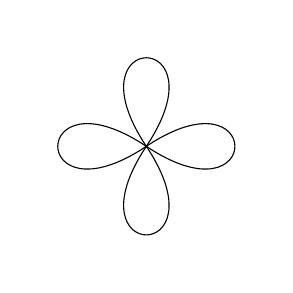
\begin{tikzpicture}[baseline=(current bounding box.center)]
		\draw (0,0) .. controls (1, 1.5) and (-1, 1.5) .. (0,0);
		\draw[rotate=90] (0,0) .. controls (1, 1.5) and (-1, 1.5) .. (0,0);
		\draw[rotate=180] (0,0) .. controls (1, 1.5) and (-1, 1.5) .. (0,0);
		\draw[rotate=270] (0,0) .. controls (1, 1.5) and (-1, 1.5) .. (0,0);
	\end{tikzpicture}\]
	我们断言存在群同构 $\mathbf{F}(X) \rightiso \pi_1(B_X, \star)$, 它将 $x \in X$ 映至 $B_X$ 中从 $\star$ 出发, 沿第 $x$ 份 $\mathbb{S}^1$ 顺向绕一圈的道路. 当 $|X|=1$ 时这无非是习见的同构 $\pi_1(\mathbb{S}^1, \star) \rightiso \Z$ \cite[第四章 \S 3.1]{You}. 一般情形则从 van Kampen 定理导出, 其有限版本可见 \cite[附录B]{You}.

	回顾图的概念. 一个图 $\Gamma = (V, E, s, t)$ 是由顶点集 $V$ 和边集 $E$ 组成的, 边有头尾两端, 由一对映射 $s, t: E \to V$ 给出. 从 $\Gamma$ 可以构造其几何实现 $|\Gamma|$: 说穿了, 这无非是对每个边具体地取一份区间 $[0, 1]$, 并沿顶点黏合成 $|\Gamma|$. 以下等同 $\Gamma$ 与 $|\Gamma|$, 所论的图因之是无向的. 先前定义的 $B_X$ 就是仅有一个顶点的图. 图论的一个基本结果断言当 $\Gamma$ 连通时, 必存在极大子树 $T$: 它是 $\Gamma$ 的子图, 包含 $\Gamma$ 的每个顶点并且不含回路. 直观地看, 我们可以在 $\Gamma$ 中让树 $T$ 连续地收缩到某顶点 $\star$ (这称为形变收缩, 见 \cite[第四章 \S 4.3]{You}); 譬如在下图中缩掉粗线标出的极大子树, 就得到之前的四叶幸运草.
	\begin{center}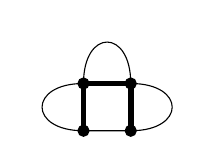
\begin{tikzpicture}[every node/.style={circle, draw, fill=black}, bentcurve/.style={bend left=90, looseness=3} ]
		\begin{scope}[scale=0.6]
			\coordinate (A) at (0,0) {};
			\coordinate (B) at (0,1) {};
			\coordinate (C) at (1,1) {};
			\coordinate (D) at (1, 0) {};
		\end{scope}
		\draw [line width=2pt] (A) -- (B) -- (C) -- (D);
		\draw[bentcurve] (A) to (B) to (C) to (D) --cycle;
		\foreach \x in {A, B, C, D}
			\draw[circle, fill=black] (\x) circle[radius=2pt];
	\end{tikzpicture}\end{center}
	一般情形下, 因 $T$ 含所有顶点, 商空间 $\Gamma/T$ 将同胚于某个 $B_Y$. 故
	\[ \pi_1(\Gamma, \star)  \rightiso \pi_1(\Gamma/T, \star) \simeq \pi_1(B_Y, \star) \; \text{是自由群}. \]
	取定集合 $X$, 复叠空间的理论 \cite[第五章 \S 4]{You} 告诉我们对 $\mathbf{F}(X) \simeq \pi_1(B_X, \star)$ 的任意子群 $H$, 皆存在复叠空间  $\widetilde{B_X} \to B_X$ 使得 $H$ 是单同态 $\pi_1\left( \widetilde{B_X}, \star \right) \to \pi_1(B_X, \star)$ 的像. 至此, 我们只消证明 $\pi_1\left(\widetilde{B_X}, \star\right)$ 自由; 断言归结为以下性质:
	\begin{center} 图的复叠空间仍为图. \end{center}
	这是复叠空间的道路提升性质的直接推论.
\end{proof}

\section{对称群}\label{sec:symmetric-group}
对集合 $X$, 其\emph{对称群} $\mathfrak{S}_X$ 是全体双射 $X \xrightarrow{1:1} X$ 对映射合成所构成的群, 它自然地左作用于 $X$ 上, 其中元素也称为置换. 本节仅关心 $n := |X|$ 有限的情形, 此时 $|\mathfrak{S}_X| = n!$. 习惯上经常将 $X$ 的元素等同于 $\{1, \ldots, n\}$ 并记 $\mathfrak{S}_n := \mathfrak{S}_{\{1, \ldots, n\}}$. 

对集合 $X$, $Y$ 存在自然的群嵌入 $\mathfrak{S}_X \times \mathfrak{S}_Y \hookrightarrow \mathfrak{S}_{X \sqcup Y}$, 或记作 $\mathfrak{S}_n \times \mathfrak{S}_m \hookrightarrow \mathfrak{S}_{n+m}$. 这里 $\mathfrak{S}_X$ 和 $\mathfrak{S}_Y$ 在 $\mathfrak{S}_{X \sqcup Y}$ 中之所以对乘法交换, 是因为它们所挪动的元素``不交''. 这自然地导向下述定义.

\begin{definition}\index{duichengqun}\index{xunhuan@循环 (cycle)}\index{duihuan@对换 (transposition)} \index[sym1]{S_n@$\mathfrak{S}_n$}
	设 $a_1, \ldots, a_m$ 是 $X$ 中相异的元素. 对称群 $\mathfrak{S}_X$ 中的 $m$-\emph{循环} (又称轮换) $(a_1 \cdots a_m)$ 是下述映射 $\sigma: X \to X$
	\begin{gather*}
		\sigma(a_i) = a_{i+1}, \quad i \in \Z/m\Z, \\
		\sigma(x)=x, \quad x \notin \{a_1, \ldots, a_m\},
	\end{gather*}
	在此将下标 $\{1, \ldots, m\}$ 方便地视为 $\Z/m\Z$ 中元素, 即模 $m$ 的同余类. 称 $m$ 为该循环的长度; $2$-循环 $(a b)$ 又称\emph{对换}. 我们称 $\mathfrak{S}_X$ 中两个循环 $(a_1 \cdots a_m)$, $(b_1 \cdots b_k)$ 不交, 如果 $\{a_1, \ldots, a_m\} \cap \{b_1, \ldots, b_k\} = \emptyset$. 
\end{definition}
由先前讨论可知不交的循环对乘法相交换. 同样显然的是 $\text{ord}((a_1 \cdots a_m)) = m$.

\begin{proposition}[循环分解]\label{prop:cyclic-decomposition}
	每个 $\sigma \in \mathfrak{S}_X$ 都能表成不交的循环之积
	\[ \sigma = (a_1 a_2 \cdots) (b_1 b_2 \cdots) \cdots \]
	其中的循环 $(a_1 \cdots)$, $(b_1 \cdots)$ 在至多差一个顺序的意义下唯一. 由于 $1$-循环是单位元, 乘积中可以省去.
\end{proposition}
\begin{proof}
	这无非是 $X$ 在 $\sigma$ 生成的有限循环群 $\lrangle{\sigma}$ 下的轨道分解 (引理 \ref{prop:orbit-decomp}), 每个循环对应到一个轨道, 描述了 $\sigma$ 在该轨道上的作用.
\end{proof}

我们称循环分解中出现的循环长度 $n_1, n_2, \ldots$ (包括长度为一的循环) 为 $\sigma$ 的循环型, 计重数不计顺序. 为了得到唯一性, 不妨排成 $n_1 \geq n_2 \geq \cdots$, 循环型因之对应于整数 $n := |X|$ 的分拆: $n = n_1 + n_2 + \cdots$. 上面对阶数的讨论蕴涵 $\sigma$ 的阶数等于 $n_1, n_2, \ldots$ 的最小公倍数. \index{fenchai@分拆 (partition)}

据此, 共轭作用在对称群情形下有干净的陈述.
\begin{lemma}\label{prop:cycle-type}
	设 $\tau = (a_1 a_2 \cdots) (b_1 \cdots) \cdots$ 为上述的循环分解, $\tau \in \mathfrak{S}_X$, 则
	\[ \sigma \tau \sigma^{-1} = (\sigma(a_1) \sigma(a_2) \cdots) (\sigma(b_1) \cdots) \cdots. \]
	作为推论, 元素 $\tau$ 的共轭类由其循环型确定; $\mathfrak{S}_X$ 中的共轭类一一对应于循环型 $n_1 \geq n_2 \geq \cdots$, 后者又一一对应于整数 $n = |X|$ 的分拆.
\end{lemma}
\begin{proof}
	易见 $\sigma \tau \sigma^{-1}$ 将 $\sigma(a_i)$ 映至 $\sigma(a_{i+1})$, 将 $\sigma(b_j)$ 映至 $\sigma(b_{j+1})$, 依此类推. 由于 $\sigma$ 是双射, 由此唯一确定了 $\sigma \tau \sigma^{-1}$ 的循环分解. 适当选取 $\sigma$ 即可使 $\sigma\tau\sigma^{-1}$ 成为任意与 $\tau$ 有同样循环型的元素, 证毕. 
\end{proof}

下面我们改采符号 $\mathfrak{S}_n$.
\begin{lemma}\label{prop:S_n-generation}
	群 $\mathfrak{S}_n$ 由对换 $\tau_i = (i \quad i+1)$ 生成, 这里 $1 \leq i < n$.
\end{lemma}
\begin{proof}
	将给定的置换 $\sigma$ 视同数列 $\sigma(1), \ldots, \sigma(n)$, 则表 $\sigma$ 为诸 $\tau_i$ 的积相当于借由反复交换数列中的相邻项, 将 $\sigma(1), \ldots, \sigma(n)$ 逐步化成 $1, \ldots, n$; 这当然是可行的. 严格论证留给有闲情逸致的读者.
\end{proof}

\begin{lemma}\index[sym1]{sgn@$\sgn$}
	存在唯一的群同态 $\sgn: \mathfrak{S}_n \to \{\pm 1\}$ 使得 $\sgn((a_1 \cdots a_m)) = (-1)^{m+1}$.
\end{lemma}
\begin{proof}
	群 $\mathfrak{S}_n$ 在函数集 $\{ f: \Z^n \to \Z\}$ 上有自然的左作用
	\[ (\sigma f)(x_1, \ldots, x_n) = f(x_{\sigma(1)}, \ldots, x_{\sigma(n)}), \]
	此作用对函数的逐点加法显然为线性: $\sigma(f \pm g) = \sigma f \pm \sigma g$. 今考虑函数
	\[ \Delta(x_1, \ldots, x_n) = \prod_{1 \leq i < j \leq n} (x_j - x_i). \]
	对于 $\sigma \in \mathfrak{S}_n$, 显见存在 $\sgn(\sigma) \in \{\pm 1\}$ 使得 $\sigma \Delta = \sgn(\sigma)\Delta$. 因为 $\Delta$ 不恒为零 (代入 $x_i = i$ 可知), $\sgn(\sigma)$ 是唯一确定的, 因而 $\sgn: \mathfrak{S}_n \to \{\pm1 \}$ 是群同态. 容易验证对每个 $1 \leq i < n$ 皆有 $\tau_i \Delta = -\Delta$. 对换之间两两共轭, 故对所有对换 $\tau \in \mathfrak{S}_n$ 皆有 $\sgn(\tau)=-1$. 由
	\[(a_1 \cdots a_m) = (a_1 a_m) (a_1 \cdots a_{m-1}) = \cdots = (a_1 a_m) (a_1 a_{m-1}) \cdots (a_1 a_2) \]
	可见 $\sgn((a_1 \cdots a_m)) = (-1)^{m+1}$. 唯一性导自命题 \ref{prop:cyclic-decomposition}. 
\end{proof}

\begin{definition}[交错群]\index[sym1]{A_n@$\mathfrak{A}_n$}
	定义\emph{交错群} $\mathfrak{A}_n$ 为 $\Ker[ \mathfrak{S}_n \xrightarrow{\sgn} \{\pm 1\}]$, 它是 $\mathfrak{S}_n$ 的正规子群.
\end{definition}
落在 $\mathfrak{A}_n$ 中的置换称为偶置换, 否则称为奇置换. 当 $n > 1$ 时 $(\mathfrak{S}_n : \mathfrak{A}_n) = |\{\pm 1\}| = 2$. 当 $n \geq 4$ 时 $\mathfrak{A}_n$ 非交换, 例如: $(1 2 3)(1 2 4) = (1 3) (2 4)$ 而 $(1 2 4)(1 2 3) = (1 4) (2 3)$.

我们需要以下简单的性质:
\begin{itemize}
	\item 群 $\mathfrak{S}_n$ 的导出子群 (见 \S\ref{sec:solvable-groups}) $\mathscr{D}^1 \mathfrak{S}_n$ 等于 $\mathfrak{A}_n$. 当 $n=1$ 时此为显然. 以下解释 $n \geq 2$ 情形: $\mathfrak{S}_n$ 由对换生成, 每个对换都共轭于 $(1 \; 2)$, 故交换商 $\mathfrak{S}_n / \mathscr{D}^1 \mathfrak{S}_n$ 由 $(1 \; 2)$ 的像生成, 这是二阶元. 另一方面引理 \ref{prop:abelianization} 给出满同态
		\[ \mathfrak{S}_n / \mathscr{D}^1 \mathfrak{S}_n \stackrel{\text{商同态}}{\twoheadrightarrow} \mathfrak{S}_n/\mathfrak{A}_n \simeq \{ \pm 1\}. \]
		比较阶数可见以上同态实为同构, 亦即 $\mathscr{D}^1 \mathfrak{S}_n = \mathfrak{A}_n$.
	\item 所有 $\mathfrak{S}_n$ 中长度为奇数的循环皆包含于 $\mathfrak{A}_n$.
	\item 当 $n \geq 3$ 时, $\mathfrak{A}_n$ 由 $3$-循环 (形如 $(i j k)$) 生成. 这是由于任意 $\sigma \in \mathfrak{A}_n$ 可以表成对换的积, $\sgn(\sigma)=1$ 确保乘积有偶数个项. 运用以下观察
		\[ (i j)(k l) = \begin{cases}
			1, & \{i,j\} = \{k,l\}, \\
			\text{$3$-循环}, & \{i,j\} \cap \ \{k,l\}\; \text{恰有一元素}, \\
			(i j k) (j k l), & \{i,j\} \cap \ \{k,l\} = \emptyset
		\end{cases} \]
		可将乘积改写为 $3$-循环的积.
	\item 当 $n \geq 5$ 时, 任两个 $3$-循环 $(i j k)$, $(i' j' k')$ 在 $\mathfrak{A}_n$ 中共轭. 首先留意到引理 \ref{prop:cycle-type} 蕴涵存在 $\sigma \in \mathfrak{S}_n$ 使得 $\sigma (i j k) \sigma^{-1} = (i' j' k')$. 若 $\sigma \in \mathfrak{A}_n$ 则收工, 否则取相异元 $l, m \in \{1, \ldots, n\} \smallsetminus \{i,j,k\}$ 并置 $\sigma' := \sigma \cdot (l m) \in \mathfrak{A}_n$; 对之仍有 $\sigma' (i j k) (\sigma')^{-1} = (i' j' k')$.
\end{itemize}
以下记任意置换 $\sigma$ 的不动点集为 $\text{Fix}(\sigma) := \left\{ i: \sigma(i)=i \right\}$.

\begin{theorem}[É.\ Galois]\label{prop:A_n-simple}
	当 $n \geq 5$ 时 $\mathfrak{A}_n$ 是单群.
\end{theorem}
\begin{proof}
	设 $H \lhd \mathfrak{A}_n$, $H \neq \{1\}$. 从以上性质可知找出一个 $3$-循环 $\sigma \in H$ 即足. 兹断言取 $\sigma \in H \smallsetminus \{1\}$ 使得 $\left|\text{Fix}(\sigma)\right|$ 极大便是.
	
	如果 $\sigma$ 的循环分解中只有对换, 那么分解中至少含两项如 $(i j) (k l)$, 其中 $\{i,j\} \cap \{k,l\} = \emptyset$. 由于 $n \geq 5$, 可取 $r \notin \{i,j,k, l\}$ 并定义
	\begin{equation}\label{eqn:tau-sigma-simple}
		\tau := (k l r), \quad \sigma' := [\tau, \sigma] = \tau\sigma\tau^{-1}\sigma^{-1} \in H \quad (\because H \lhd \mathfrak{A}_n).
	\end{equation}
	可直接验证 $i,j \in \text{Fix}(\sigma') \smallsetminus \text{Fix}(\sigma)$, $\sigma'(k) = r \neq k$, 以及
	\[ \text{Fix}(\sigma) \smallsetminus \{r\} = \text{Fix}(\sigma) \smallsetminus \{k, l, r\} = \text{Fix}(\sigma) \cap \text{Fix}(\tau) \subset \text{Fix}(\sigma'). \]
	综之 $\left|\text{Fix}(\sigma')\right| > \left|\mathrm{Fix}(\sigma)\right|$, 矛盾.
	
	设 $\sigma$ 的循环分解中包含长度 $>2$ 的项 $(i j k \cdots)$. 假若 $\sigma = (i j k)$ 则是所求的 $3$-循环; 否则因为 $\sigma$ 不可能是 $4$-循环, $\sigma$ 除了 $i,j,k$ 之外还挪动至少两个相异元 $r, l$. 依然以 \eqref{eqn:tau-sigma-simple} 式定义 $\sigma' \in H$. 可以验证 $j \in \text{Fix}(\sigma')$, $\sigma'(k) = l \neq k$ 和
	\[ \text{Fix}(\sigma) = \text{Fix}(\sigma) \smallsetminus \{k,l,r\} = \text{Fix}(\sigma) \cap \text{Fix}(\tau) \subset \text{Fix}(\sigma'). \]
	仍得到矛盾 $\left|\text{Fix}(\sigma')\right| > \left|\mathrm{Fix}(\sigma)\right|$. 明所欲证.
\end{proof}

当 $n \geq 5$ 时 $\mathfrak{A}_n$ 是非交换单群, 因此它必然等于自身的导出子群 $\mathscr{D}^1 \mathfrak{A}_n$. 下述推论是证明五次以上方程无根式解 (定理 \ref{prop:Abel-Ruffini}) 的群论钥匙.
\begin{corollary}\label{prop:S_n-unsolvable}\index{kejiequn}
	当 $n \geq 5$ 时, 对所有 $i \geq 1$ 都有 $\mathscr{D}^i \mathfrak{S}_n = \mathfrak{A}_n$; 作为推论, 当 $n \geq 5$ 时 $\mathfrak{S}_n$ 不可解.
\end{corollary}
\begin{proof}
	已知 $\mathscr{D}^1 \mathfrak{S}_n = \mathfrak{A}_n$. 配合前述讨论, 当 $n \geq 5$ 时, 对所有 $i \geq 1$ 皆有 $\mathscr{D}^i \mathfrak{S}_n = \mathscr{D}^{i-1} \mathfrak{A}_n = \mathfrak{A}_n$. 关于不可解性的断言请见引理 \ref{prop:solvable-nilpotent-characterization}.
\end{proof}

读者可以动手验证 $\mathscr{D}^1 \mathfrak{A}_4 = \left\{\identity, (1 2)(3 4), (1 3) (2 4), (1 4)(2 3)\right\}$, 同构于 $(\Z/2\Z)^2$. 因此 $n < 5$ 时 $\mathfrak{S}_n$ 确实可解.

我们接着考察 $\mathfrak{S}_n$ 的展示. 为此不妨一并考虑例 \ref{eg:braid} 提到的辫群 $\mathcal{B}_n$. 简要摘录之前的构造如下: 形象地看, $\mathcal{B}_n$ 是由所有 $n$ 条线编成的辫子为元素的群, 辫子在空间 $\R^3$ 中连续的形变下 (不动端点, 不割断线) 视为等价. 辫子可以图解为诸如 ($n=2,3$)
\begin{center}\begin{tikzpicture}[baseline=(braid)]
	\braid[style strands={1}, style strands={2}] (braid) s_1;
	\end{tikzpicture} \qquad \begin{tikzpicture}[baseline=(braid), yscale=0.8]
	\braid[style strands={1}, style strands={2}, style strands={3}] (braid)  s_1 s_2^{-1};
\end{tikzpicture}\end{center}
的形式. 辫群中的乘法是将辫子从上而下地接合, 如
\begin{center}\begin{tikzpicture}[baseline=(braid)]
	\braid[style strands={1}, style strands={2}] (braid) s_1;
	\end{tikzpicture} \quad $\bullet$ \quad \begin{tikzpicture}[baseline=(braid)]
	\braid[style strands={1}, style strands={2}] (braid) s_1^{-1};
	\end{tikzpicture} \quad $=$ \quad \begin{tikzpicture}[baseline=(braid), yscale=0.8]
	\braid[style strands={1}, style strands={2}] (braid) s_1 s_1^{-1};
	\end{tikzpicture} \quad $\xlongequal{\text{拉直}}$ \quad
	\begin{tikzpicture}[baseline=(M), yscale=0.8]
	\draw (0,1) -- (0,-1);
	\draw (1,1) -- (1,-1);
	\coordinate (M) at (0,0);
\end{tikzpicture}\end{center}
结合律一望可知, $\mathcal{B}_n$ 的幺元是 $n$ 条平行线 $\vert \cdots \vert$. 辫子的图表对水平轴作镜射给出其逆, 何以故? 请端详上图.

两组辫子的``横向并列''导出群同态 $\mathcal{B}_n \times \mathcal{B}_m \to \mathcal{B}_{n+m}$.

显然 $\mathcal{B}_1 = \{1\}$. 以下假设 $n \geq 2$. 对 $1 \leq i < n$, 定义元素 $\sigma_i \in \mathcal{B}_n$ 使得其中第 $i$, $i+1$ 条线的缠绕模式为
\begin{center} \begin{tikzpicture}
	\braid[style strands={1}, style strands={2}] (braid) s_1;
	\node[above] at (braid-1-s) {$i$};
	\node[above] at (braid-2-s) {$i+1$};
\end{tikzpicture} \end{center}
其余诸线则不相缠绕. 容易看出当 $|i-j| > 1$ 时, $\sigma_i$, $\sigma_j$ 影响的线不交故 $\sigma_i \sigma_j = \sigma_j \sigma_i$; 另一方面, ``杨--Baxter 方程''
\[ \begin{tikzpicture}[yscale=0.6, baseline=(braid)]
	\braid[style strands={1}, style strands={2}, style strands={3}] (braid) s_1 s_2 s_1;
	\node[above] at (braid-1-s) {$i$};
	\node[above] at (braid-2-s) {$i+1$};
	\node[above] at (braid-3-s) {$i+2$};
	\end{tikzpicture}
	\qquad = \qquad
	\begin{tikzpicture}[yscale=0.6, baseline=(braid)]
	\braid[style strands={1}, style strands={2}, style strands={3}] (braid) s_2 s_1 s_2;
	\node[above] at (braid-1-s) {$i$};
	\node[above] at (braid-2-s) {$i+1$};
	\node[above] at (braid-3-s) {$i+2$};
\end{tikzpicture} \]
表明 $\sigma_i \sigma_{i+1} \sigma_i = \sigma_{i+1} \sigma_i \sigma_{i+1}$ 对 $1 \leq i < n-1$ 恒成立. 请读者试着直观地理解
\begin{inparaenum}[(a)]
	\item 元素 $\sigma_1, \ldots, \sigma_{n-1}$ 生成 $\mathcal{B}_n$,
	\item 关系式 $|i-j| > 1 \implies \sigma_i \sigma_j = \sigma_j \sigma_i$ 和 $\sigma_i \sigma_{i+1} \sigma_i = \sigma_{i+1} \sigma_i \sigma_{i+1}$ 完全描述了 $\mathcal{B}_n$ 的结构.
\end{inparaenum}
更精简的说法是借助群的展示
\begin{equation}\label{eqn:braid-presentation} \left\langle \sigma_1, \ldots, \sigma_{n-1} \Biggr| \begin{array}{ll}
	\sigma_i \sigma_j = \sigma_j \sigma_i, & |i-j| > 1 \\
	\sigma_i \sigma_{i+1} \sigma_i = \sigma_{i+1} \sigma_i \sigma_{i+1}, & 1 \leq i < n-1
	\end{array} \right\rangle \rightiso \mathcal{B}_n. \end{equation}

这个展示既可以从 $\mathcal{B}_n$ 的拓扑诠释推导, 亦可直接当作辫群的组合学定义. 留意到 $\mathcal{B}_2 \simeq \Z$, 当 $n \geq 3$ 时 $\mathcal{B}_n$ 是无穷非交换群.

现在我们来联系 $\mathcal{B}_n$ 与 $\mathfrak{S}_n$. 对每条辫子 $x \in \mathcal{B}_n$, 定义相应的 $\sigma \in \mathfrak{S}_n$ 使得辫图从底端 $i$ 走到顶端 $\sigma(i)$ 如下
\begin{center}\begin{tikzpicture}[scale=0.5]
	\node (S) at (-1.7, 1) {$\sigma(i)$};
	\node (E) at (1.7, -1) {$i$};
	\draw (S) -- (E) node[midway, fill=white, anchor=center, sloped] {$\cdots$};
\end{tikzpicture}\end{center}
易见这给出群同态 $\mathcal{B}_n \to \mathfrak{S}_n$, 它使图表
\[\begin{tikzcd}
	\mathcal{B}_n \times \mathcal{B}_m \arrow[r] \arrow[d] & \mathcal{B}_{n+m} \arrow[d] \\
	\mathfrak{S}_n \times \mathfrak{S}_m \arrow[r] & \mathfrak{S}_{n+m}
\end{tikzcd}\]
交换, 并将 $\sigma_i \in \mathcal{B}_n$ 映到对换
\[ \tau_i := (i \quad i+1) \in \mathfrak{S}_n, \quad 1 \leq i < n. \]
引理 \ref{prop:S_n-generation} 断言它们生成 $\mathfrak{S}_n$. 如改从 $\mathcal{B}_n$ 的展示 \eqref{eqn:braid-presentation} 切入, 我们可以先在 $\mathfrak{S}_n$ 中验证关系式
\begin{gather*}
	|i-j| > 1 \implies \tau_i \tau_j = \tau_j \tau_i, \\
	\tau_i^2 = 1, \quad 1 \leq i < n, \\
	\tau_i \tau_{i+1} \tau_i = \tau_{i+1} \tau_i \tau_{i+1} = (i \quad i+2), \quad 1 \leq i < n-1.
\end{gather*}
所以 $\sigma_i \mapsto \tau_i$ 确定了同态 $\mathcal{B}_n \to \mathfrak{S}_n$. 这就引出一个显然的问题: 这些关系式是否给出 $\mathfrak{S}_n$ 的展示?

为避免歧义, 另立符号 $\tilde{\tau}_i$ 代入以上三族关系式, 联立后能够化作等价形式
\begin{equation}\label{eqn:S_n-presentation}\begin{gathered}
	\tilde{\tau}_i^2 = 1, \quad 1 \leq i < n \\
	|i-j| > 1 \implies (\tilde{\tau}_i \tilde{\tau}_j)^2 = 1, \\
	(\tilde{\tau}_i \tilde{\tau}_{i+1})^3 = 1, \quad 1 \leq i < n-1.
\end{gathered}\end{equation}
定义 $\mathfrak{S}'_n := \lrangle{\tilde{\tau}_1, \ldots, \tilde{\tau}_n \big| \text{满足于}\; \eqref{eqn:S_n-presentation} }$, 另外约定 $\mathfrak{S}'_1 := \{1\}$. 因之有群同态 $\mathcal{B}_n \twoheadrightarrow \mathfrak{S}'_n \twoheadrightarrow \mathfrak{S}_n$, 满足 $\sigma_i \mapsto \tilde{\tau}_i \mapsto \tau_i$. 从 $\mathcal{B}_n$ 过渡到 $\mathfrak{S}'_n$ 相当于忽视缠绕
\begin{tikzpicture}[baseline=(braid), yscale=0.5, xscale=0.7]
	\braid[style strands={1}, style strands={2}] (braid) s_1 s_1;
\end{tikzpicture}.

\begin{theorem}\label{prop:S_n-presentation}
	映射 $\mathfrak{S}'_n \to \mathfrak{S}_n$ 是同构, 换言之 \eqref{eqn:S_n-presentation} 确实给出 $\mathfrak{S}_n$ 的展示.
\end{theorem}
\begin{proof}
	既然 $\mathfrak{S}'_n \to \mathfrak{S}_n$ 是满同态, 只要递归地证明 $|\mathfrak{S}'_n| \leq n!$ 即可. 因 $n=1,2$ 的情形是平凡的, 以下设 $n > 2$. 展示 \eqref{eqn:S_n-presentation} 给出自然同态 $\mathfrak{S}'_{n-1} \to \mathfrak{S}'_n$. 我们暂不知这是否为单射, 但总能让 $\mathfrak{S}'_{n-1}$ 以右乘作用在 $\mathfrak{S}'_n$ 上并考察其轨道. 今断言
	\[ \mathfrak{S}'_n = 1 \cdot \mathfrak{S}'_{n-1} \cup \tilde{\tau}_{n-1}\mathfrak{S}'_{n-1} \cup \cdots \cup (\tilde{\tau}_1 \cdots \tilde{\tau}_{n-1} \mathfrak{S}'_{n-1}), \]
	若此式成立, 立得 $\mathfrak{S}'_n \leq n |\mathfrak{S}'_{n-1}| \leq n(n-1)! = n!$.
	
	仅须证明等式右侧在每个 $\tilde{\tau}_i$ 的左乘下保持封闭. 考虑 $\tilde{\tau}_i (\tilde{\tau}_j \cdots \tilde{\tau}_{n-1}) \mathfrak{S}'_{n-1}$: 当 $i=j-1$ 或 $i=j$ 时显然有封闭性 ($\tilde{\tau}_j^2 = 1$); 当 $i < j-1$ 时用 \eqref{eqn:S_n-presentation} 可将 $\tilde{\tau}_i$ 朝右吸收到 $\mathfrak{S}'_{n-1}$, 依然封闭. 故以下假设 $i>j$. 我们利用 \eqref{eqn:S_n-presentation} 的第二式将 $\bm{\tilde{\tau}_i}$ 右移 (为强调故变化字体), 直到
	\[ \cdots \tilde{\tau}_{i-2} \bm{\tilde{\tau}_i} \tilde{\tau}_{i-1} \tilde{\tau}_i \tilde{\tau}_{i+1} \cdots \mathfrak{S}'_{n-1}. \]
	接着应用 \eqref{eqn:S_n-presentation} 的第三式 (或它在 \eqref{eqn:braid-presentation} 中的形式) 化之为
	\[ \cdots \tilde{\tau}_{i-2} \tilde{\tau}_{i-1} \tilde{\tau}_i \bm{\tilde{\tau}_{i-1}} \tilde{\tau}_{i+1} \cdots \mathfrak{S}'_{n-1}. \]
	上式标出的 $\bm{\tilde{\tau}_{i-1}}$ 可一路右移直到并入 $\mathfrak{S}'_{n-1}$, 故所求的左乘封闭性成立.
\end{proof}

展示 \eqref{eqn:S_n-presentation} 表明对称群属于一类称为 Coxeter 群的构造, 它们带有形如 $W = \lrangle{S \big| (st)^{m(s,t)}=1, \; s,t \in S}$ 的展示, 其中
\begin{compactitem}
	\item $S$ 是有限集,
	\item $m: S \times S \to \Z_{\geq 1} \sqcup \{\infty\}$ (取 $\infty$ 意谓无关系),
	\item $\forall s,t \in S, \; m(s,t)=m(t,s)$,
	\item $s=t \iff m(s,t)=1$.
\end{compactitem}
例 \ref{eg:dihedral-presentation} 表明二面体群 $D_{2n}$ 也具有这种展示. Coxeter 群是研究 Lie 群, Lie 代数和相关表示理论的必备工具. \index{Coxeter 群}

\section{群的极限和完备化}\label{sec:group-limit}
基于 \S\ref{sec:free-group} 的构造和例 \ref{eg:complete-cocomplete}, 群范畴 $\cate{Grp}$ 和其子范畴 $\cate{Ab}$ 中可以定义极限 $\varinjlim$ 和 $\varprojlim$. 构造方法已在例 \ref{eg:complete-cocomplete} 大致说明. 本节将深入探讨 $\varprojlim$ 的情形.

对于小范畴 $I$, 给定函子 $\beta: I^\text{op} \to \cate{Grp}$ 相当于给定一族群 $\{ G_i := \beta(i) : i \in \Obj(I) \}$, 并对每个箭头 $s: i \to j$ 指定群同态 $\beta(s): G_j \to G_i$, 使得
\begin{compactitem}
	\item $\beta(\identity: i \to i)=\identity_{G_i}$,
	\item 合成箭头 $i \to j \to k$ 给出合成同态 $G_k \to G_j \to G_i$.
\end{compactitem}
例 \ref{eg:complete-cocomplete} 已将 $\varprojlim_i G_i := \varprojlim \beta$ 的存在性归结为积和等化子的存在性. 铺开定理 \ref{prop:limit-buildingblocks} 证明中的构造, 便得到明白的表法
\[
	\varprojlim_i G_i := \left\{ (x_i)_{i \in I} \in \prod_{i \in I} G_i : \forall s: i \to j, \; \beta(s)(x_j) = x_i \right\}.
\]
显然 $\varprojlim_i G_i$ 构成直积 $\prod_{i \in I} G_i$ 的子群. 同时我们也得到自明的投影同态 $p_j: \varprojlim_i G_i \to G_j$.

以下将假设 $I$ 实由偏序集 $(I, \leq)$ 给出 (参看例 \ref{eg:categories}); 并且 $(I, \leq)$ 是\emph{滤过}的, 即任意两元素都有共同上界 (定义 \ref{def:filtrant-poset}). 滤过偏序是滤过范畴的一个特例, 请见定义 \ref{def:filtrant-cat}.\index{luguoxuji}

首先回顾一些点集拓扑学的定义, 详见 \cite[第一章]{FL14}.
\begin{definition}\label{def:topological-group}\index{tuopuqun@拓扑群 (topological group)}
	一个拓扑群 $G$ 意指群 $G$ 上带有拓扑结构, 使得乘法 $m: G \times G \to G$ 与取逆运算 $i: G \to G$ 皆为连续映射.
\end{definition}
典型例子是加法群 $(\R^n, +)$. 作为推论, 任意 $g \in G$ 的左乘或右乘作用都给出同胚 $G \to G$, 取逆亦同. 基于此, 群的拓扑完全由幺元 $1$ 的邻域基反映, 因为总能以左右乘法将基平移到 $G$ 的每一点, 而且 $1$ 的一组邻域基各个取逆后仍是邻域基. 反过来, 给定群 $G$ 的一族子集 $\{H_i \ni 1\}_{i \in I}$, 能否靠左右平移赋予 $G$ 拓扑群结构, 并使该子集给出 $1$ 处的开邻域基? 以下情形对我们已经足够了: 假定 $(I, \leq)$ 是滤过偏序集, $i \leq j \implies H_j \subset H_i$ 而且 $\forall i \; H_i \lhd G$, 那么这样的拓扑总是存在: 事实上
\[ \text{子集}\; E \subset G\; \text{为开} \iff \forall x \in E, \; \exists i \in I, \; xH_i = H_i x \subset E. \]
易见这的确使 $G$ 成拓扑群, 验证留作简单习题. 进一步, 拓扑的分离性公理也简化了.

\begin{lemma}\label{prop:top-group-separation}
	设 $G$ 为拓扑群, 则
	\begin{equation}\label{eqn:top-group-Hausdorff}
		G:\; \text{Hausdorff} \iff \{1\} \subset G\; \text{为闭子集} \iff \bigcap_{U \ni 1: \text{开邻域}} U = \{1\}.
	\end{equation}
	此外, 任何 $x \in G$ 都有一组由闭邻域构成的邻域基.
\end{lemma}
\begin{proof}
	先处理第一条. 对每个 $x \in G$ 置 $\mathfrak{N}_x := \left\{ x \;\text{的所有邻域} \right\}$. 先前关于邻域基的讨论给出 $\mathfrak{N}_x = x\mathfrak{N}_1 = x \mathfrak{N}_1^{-1}$ (意谓对每个邻域都用 $x$ 平移或取逆), 从而
	\begin{equation*}\begin{aligned}
		x \in \overline{\left\{ 1 \right\}} & \iff 1 \in \bigcap_{V \in \mathfrak{N}_x} V = \bigcap_{U \in \mathfrak{N}_1} xU^{-1} \\
		& \iff x^{-1} \in \bigcap_{U \in \mathfrak{N}_1} U^{-1} \iff x \in \bigcap_{U \in \mathfrak{N}_1} U.
	\end{aligned}\end{equation*}
	换言之 $\overline{\{1\}} = \bigcap_{U \in \mathfrak{N}_1} U$. 由之立见第二个 $\iff$. 对第一个 $\iff$ 仅 $\Leftarrow$ 方向非平凡: 定义连续函数 $\nu: G \times G \to G$ 映 $(x,y)$ 为 $xy^{-1}$, 那么 $G$ 是 Hausdorff 空间等价于对角子集 $\Delta_G \subset G \times G$ 为闭, 但 $\Delta_G = \nu^{-1}(1)$ 而 $\{1\} \subset G$ 为闭.

	第二条即刻化约到 $x=1$ 的情形; 由于群运算的连续性, 对任何开邻域 $V \ni 1$ 皆存在开集 $U \ni 1$ 使得 $U^{-1}U \subset V$, 只须观察到闭包 $\bar{U}$ 包含于 $U^{-1} \cdot U$: 这是因为 $g \in \bar{U}$ 蕴涵 $Ug \cap U \neq \emptyset$.
\end{proof}

\begin{lemma}\label{prop:open-closed-subgroup}
	设拓扑群 $G$ 的子群 $H$ 是 $1$ 的邻域, 则 $H$ 既开又闭, 而且 $G$ 紧蕴涵 $(G:H)$ 有限.
\end{lemma}
\begin{proof}
	取开集 $U$ 使得 $1 \in U \subset H$, 因此 $H = \bigcup_{x \in H} Ux$ 为开. 取 $G/H$ 在 $G$ 中的一族代表元 $\Xi$, 则陪集分解 (引理 \ref{prop:coset-decomp}) 给出 $G$ 的开覆盖 $G = \bigsqcup_{x \in \Xi} xH$. 于是 $H = G \smallsetminus \bigsqcup_{\substack{x \in \Xi \\ xH \neq H}} xH$ 为闭, 而且当 $G$ 紧时 $\Xi$ 有限.
\end{proof}

回到 $\varprojlim_i G_i$. 今假设每个 $G_i$ 皆是拓扑群, 且对每个 $i \leq j$ 同态 $G_j \to G_i$ 皆连续. 我们赋 $\prod_{i \in I} G_i$ 予积拓扑 (见 \cite[\S 3.3]{Xiong}), 其子群 $\varprojlim_i G_i$ 遂继承了自然的拓扑群结构.
\begin{lemma}\label{prop:completion-compactness}
	拓扑群 $\varprojlim_i G_i$ 在 $1$ 处有一组形如
	\[ \mathcal{U}_{I_0} = \bigcap_{i \in I_0} p_i^{-1}(U_i), \qquad I_0 \subset I: \; \text{ 有限子集}, \quad U_i \ni 1: \; \text{开子集} \]
	的邻域基. 若每个 $G_i$ 都是 Hausdorff 空间, 则 $\varprojlim_i G_i$ 亦然; 如进一步假设每个 $G_i$ 皆紧, 则 $\varprojlim_i G_i$ 是紧 Hausdorff 空间.
\end{lemma}
由于已设 $(I, \leq)$ 滤过, 描述邻域基时可取 $I_0$ 的上界 $j$, 从而化约到 $I_0 = \{j\}$ 的情形.
\begin{proof}
	邻域基的描述是积拓扑定义的直接推论. Hausdorff 空间的积和子空间仍是 Hausdorff 的, 而 Tychonoff 定理 \cite[定理 7.7.2]{Xiong} 断言紧空间的积仍紧; 从 Hausdorff 性质可推出 $\varprojlim_i G_i$ 是 $\prod_i G_i$ 的闭子群 (它由一族连续函数的等式定义), 故紧.
\end{proof}

在代数及数论中, 较常见的是每个 $G_i$ 皆为有限群的情形, 此时赋予 $G_i$ 离散拓扑使之成为 Hausdorff 紧群.
\begin{definition}[pro-有限群]\label{def:profinite-group}\index{pro-youxianqun@pro-有限群 (pro-finite group)}
	同构意义下形如 $\varprojlim_i G_i$, 其中 $(I, \leq)$ 滤过而且每个 $G_i$ 皆有限的拓扑群, 称作 \emph{pro-有限群}.
\end{definition}

\begin{theorem}\label{prop:profinite-characterization}
	一个拓扑群 $G$ 是 pro-有限群当且仅当它是 Hausdorff 紧群, 而且 $1$ 处有一组由正规子群构成的邻域基.
\end{theorem}
\begin{proof}
	假设 $G = \varprojlim_i G_i$ 为 pro-有限. 我们业已说明 $G$ 为 Hausdorff 紧群. 引理 \ref{prop:completion-compactness} 中的 $U_i$ 可取为 $\{1\}$, 从而 $1$ 的邻域基由一族正规开子群 $U$ 组成.

	现假设拓扑群 $G$ 满足所示条件, 取一组正规子群构成的邻域基, 记为 $I$; 集合的包含关系使 $I$ 成为偏序集, 邻域基的性质确保 $(I, \leq)$ 滤过. 将对应于 $i \in I$ 的正规子群记为 $N_i$. 引理 \ref{prop:open-closed-subgroup} 蕴涵 $G/N_i$ 有限, $N_i$ 既开且闭.

	根据泛性质, 全体商映射 $q_i: G \to G/N_i$ 确定了同态 $\varphi: G \to \varprojlim_i G/N_i$. 我们断言 $\varphi$ 是拓扑群的同构. 首先, 不难验证 $\varphi$ 连续, 而且 Hausdorff 性质确保 $\Ker(\varphi) = \bigcap_{i \in I} N_i = \{1\}$, 故 $\varphi$ 为单射. 今断言 $\Image(\varphi)$ 在 $\varprojlim_i G/N_i$ 中稠密. 诚然, 取 $x = (x_i)_i \in \varprojlim_i G/N_i$, 对任意有限子集 $I_0 \subset I$, 仅需说明 $x^{-1} \Image(\varphi)$ 交 $\bigcap_{i \in I_0} \Ker(p_i)$. 根据滤过偏序集的定义 , 存在 $I_0$ 的一个上界 $k \in I$; 取 $y \in G$ 使得 $q_k(y) = x_k$, 那么对每个 $i \in I_0$ 都会有 $q_i(y) = x_i$, 因而 $x^{-1} \varphi(y) \in \bigcap_{i \in I_0} \Ker(p_i)$.

	由于 $G$ 和 $\varprojlim_i G/N_i$ 都是紧 Hausdorff 空间, 综上 $\varphi$ 自动成为同胚 (见 \cite[\S 7.2]{Xiong}). 明所欲证.
\end{proof}
\begin{remark}\label{rem:totally-disconnected}
	以上条件可以化成更有拓扑味儿的形式: $G$ 为 pro-有限当且仅当 $G$ 是完全不连通的紧群. 证明见 \cite[命题 1.9.3]{FL14}.
\end{remark}

\begin{definition}[群的完备化]\label{def:group-completion} \index{wanbeihua@完备化 (completion)}
	设 $G$ 为群. 假设偏序集 $(I, \leq)$ 滤过. 对每个 $i \in \Obj(I)$ 取定正规子群 $H_i \lhd G$, 并假设 $i \leq j \implies H_j \subset H_i$. 则在 $\varprojlim$ 的定义中可取 $G_i := G/H_i$, 而且 $i \leq j$ (即 $i \to j$) 给出商同态 $G/H_j \twoheadrightarrow G/H_i$. 极限 $\varprojlim_i G/H_i$ 称作 $G$ 对子群族 $(H_i)_{i \in I}$ 的\emph{完备化}.
\end{definition}
完备化带有显然的同态 $\iota: G \xrightarrow{g \mapsto (gH_i)_{i \in I}} \varprojlim_i G/H_i$. 以下概略解释``完备化''与拓扑的关联. 简单起见, 今后假定偏序集 $I$ 可数. 读者对于以 Cauchy 列从 $\Q$ 构造 $\R$ 的手法理应有基本的认知.
\begin{definition}
	拓扑群 $G$ 中的点列 $(x_n)_{n \geq 0}$ 称为 \emph{Cauchy 列}, 如果对任意 $1$ 的开邻域 $U$, 存在 $N \geq 0$ 使得 $n, m \geq N \implies x_n x_m^{-1} \in U$. 假定 $G$ 在 $1$ 处有一组可数邻域基, 如果群 $G$ 的每个 Cauchy 序列都收敛, 则称 $G$ 为\emph{完备}的.
\end{definition}

今后总假设有 $1$ 的可数邻域基. 考虑 $G$ 在拓扑意义下的完备化: 这系指一个拓扑群的同态 $\iota: G \to \hat{G}$, 满足下述性质:
\begin{enumerate}[\bfseries {CO}.1]
	\item $\iota: G \to \iota(G) \subset \hat{G}$ 是同胚;
	\item $\iota$ 的像稠密;
	\item $\hat{G}$ 是完备的 Hausdorff 拓扑群.
\end{enumerate}
完备化的构造方式不止一种, 要旨在于性质 \textbf{CO.1} --- \textbf{CO.3} 唯一刻画了 $(\hat{G}, \iota)$, 精确到一个唯一同构; 其证明可以参照大同小异的命题 \ref{prop:completion-ring-characterization}, 或度量空间情形 \cite[\S 8.1]{Xiong}. 如直观地把握, 则这三条性质说明 $\hat{G}$ 中元素可以用 $G$ 中的 Cauchy 列代表, 而且只要 $\hat{x}, \hat{y} \in \hat{G}$ 足够接近, 则 $G$ 中以之为极限的 Cauchy 列 $(x_n)_n$, $(y_n)_n$ 也会足够接近 (当 $n \gg 0$); 于是 $\hat{G}$ 的结构完全被 $G$ 确定. 如此则思过半矣.

\begin{theorem}
	考虑定义 \ref{def:group-completion} 中的资料 $\{ H_i \lhd G \}_{i \in I}$ 并假定 $\bigcap_i H_i = \{1\}$, 赋予 $G$ 以 $\{H_i : i \in I \}$ 为 $1$ 的邻域基之 Hausdorff 拓扑群结构, 并赋予每个 $G/H_i$ 离散拓扑. 进一步设 $I$ 可数, 则 $\iota: G \to \varprojlim_i G/H_i$ 满足 \textbf{CO.1} --- \textbf{CO.3}, 因而也是拓扑意义下的完备化.
\end{theorem}
\begin{proof}
	可数条件蕴涵 $G$ 和 $\hat{G} := \varprojlim_i G/H_i$ 在幺元处确实有可数邻域基. 由 $\Ker(\iota) = \bigcap_i H_i = \{1\}$ 知 $\iota$ 为单. 引理 \ref{prop:completion-compactness} 中 $\hat{G}$ 的邻域基 $\mathcal{U}_j := \{ \hat{y}=(\bar{y}_i)_i \in \hat{G}: i \leq j \implies \bar{y}_i = 1 \}$ 满足 $\iota^{-1}(\mathcal{U}_j) = H_j$, 因此得到 $\iota$ 连续和 \textbf{CO.1}. 至于 \textbf{CO.2}, 对 $\hat{x} = (\bar{x}_i)_i \in \hat{G}$ 和任给之 $j \in I$, 取 $G \ni x_j \mapsto \bar{x}_j$, 则 $\iota(x_j) \in \hat{x}\mathcal{U}_j$, 故 $\iota(G)$ 稠密.
	
	兹确立 \textbf{CO.3}. 对于 $\hat{G}$ 中 Cauchy 列 $(\hat{x}_n)_n$, 对任给之 $j$, 当 $n,m \gg 0$ 时 $\hat{x}_n \hat{x}_m^{-1} \in \mathcal{U}_j$, 故 $\hat{x}_n$ 的 $j$-分量当 $n \gg 0$ 时为常数, 记作 $\bar{x}_j \in G/H_j$. 置 $\hat{x} := (\bar{x}_i)_i \in \hat{G}$ 即为 $(\hat{x}_n)_n$ 的极限.
\end{proof}

\begin{remark}
	若舍去邻域基的可数条件, 则完备性须改以网 (Moore--Smith 收敛性) 或滤子的语言陈述, 我们将在 \S\ref{sec:filters} 引入滤子, 并回头考察 $\iota: G \to \hat{G}$ 的构造.
\end{remark}

\begin{example}[$p$-进数]\label{eg:p-adic}\index[sym1]{Z_p@$\Z_p$}
	取 $I$ 为全序集 $\Z_{\geq 0}$. 对每个 $i \geq 0$ 定义 $H_i := p^{i+1} \Z$. 完备化 $\varprojlim_i \Z/p^{i+1} \Z$ 记作 $\Z_p$, 其元素无非是一族 $(a_i \in \Z/p^{i+1} \Z)_{i \geq 1}$, 满足 $a_{i+1} \mapsto a_i$. 称此为 $p$-进数的加法群; 我们会在 \S\ref{sec:ring-limits} 探讨 $\Z_p$ 上的乘法结构.
\end{example}

\begin{example}[Tate 模]\index{Tate 模}
	设 $A$ 为交换群, $\ell$ 为素数. 仍取 $I = \Z_{\geq 0}$ 如上. 对每个 $N \in \Z$ 置 $A[N] := \Ker[a \mapsto a^N]$, 显然 $N \mid N' \implies A[N] \subset A[N']$; 置 $A[\ell^\infty] := \bigcup_{n \geq 0} A[\ell^n]$. 定义函子 $V: I^\text{op} \to \cate{Ab}$ 为
	\begin{align*}
		V(i) & := A[\ell^\infty], \\
		V(i \to i+1) & := [a \mapsto a^\ell].
	\end{align*}
	置 $V_\ell(A) := \varprojlim_i V(i)$. 其元素 $(a_i \in A[\ell^\infty])_{i \geq 0}$ 须满足 $a_{i+1}^\ell = a_i$. 称此为\emph{有理 Tate 模}. 以同样方式定义一函子 $T: I^\text{op} \to \cate{Ab}$, 但要求 $T(0) = \{1\}$, 得到的极限是
	\[ T_\ell(A) := \varprojlim_i T(i) \subset V_\ell(A), \]
	称为群 $A$ 的 \emph{Tate 模}. 请留意到 $T(i) = A[\ell^i]$.

	举例明之. 取复环面 $E := \CC \big/(\Z \oplus \Z\tau)$ 所成的加法群, 其中 $\text{Im}(\tau) > 0$. 映射 $(a,b) \mapsto a+b\tau$ 导出同构 $(\R/\Z)^2 \rightiso E$, 而 $(\R/\Z)[\ell^i] = \ell^{-i}\Z/\Z$. 易见图表
	\[ \begin{tikzcd}
		a \bmod \Z \arrow[mapsto]{r} \arrow[mapsto, bend right=60]{ddd} \arrow[phantom, d, sloped, "\in" description] & \ell^{i+1}a \bmod \ell^{i+1} \Z \arrow[mapsto, bend left=60]{ddd} \arrow[phantom, d, sloped, "\in" description] \\
		\ell^{-i-1}\Z/\Z \arrow[d, "{\text{乘以} \ell}"'] \arrow[r, "\sim"] & \Z/\ell^{i+1} \Z \arrow[d, "{\text{商}}"] \\
		\ell^{-i}\Z/\Z \arrow[r, "\sim"'] & \Z/\ell^i \Z \\
		\ell a \bmod \Z \arrow[mapsto]{r} \arrow[phantom, u, sloped, "\in" description] & \ell^{i+1} a \bmod \ell^i \Z \arrow[phantom, u, sloped, "\in" description]
	\end{tikzcd} \]
	交换, 故 $T_\ell(E) \simeq \Z_\ell \oplus \Z_\ell$. 令 $\Gamma := \Z \oplus \Z\tau$, 以上论证实则说明了 $T_\ell(E)$ 自然同构于 $\Gamma$ 对 $(\ell^i \Gamma)_{i \geq 0}$ 的完备化.

	当 $\ell$ 取遍所有素数, 不妨设想 $T_\ell(E)$ 代数地``模拟''了定义 $E$ 的格 $\Gamma$, 而后者又是 $E$ 的拓扑不变量 $H_1(E, \Z)$. 这般手法对复环面自然是迂回. 然而 $E$ 又可看作射影平面 $\mathbb{P}^2(\CC)$ 中的三次代数曲线, 连同一个给定的点 $O$ (对应于复环面的零点), 此即域 $\CC$ 上的\emph{椭圆曲线}; 后一种解读能在任意代数闭域上操作, 相应的曲线依然是交换群. 这种代数框架是处理相关数论问题所必须的, 此时不易沿用习见的同调理论, Tate 模 $T_\ell(E)$ 就成为极有力的工具.
\end{example}

\section{范畴中的群}\label{sec:group-in-cat}
群范畴 $\cate{Grp}$, $\cate{Ab}$ 的性质已经谈了不少, 现在我们反其道而行, 试着在一般范畴中辨识具有``群''特质的对象. 此节可以视为范畴论的初步练习.

以下取 $\mathcal{C}$ 为范畴, 并假设 $\mathcal{C}$ 具备有限积; 特别地, $\mathcal{C}$ 中有一个择定的终对象 $\munit$, 亦即空积.

\begin{definition}\label{def:group-object}\index{duixiang!群对象 (group object)}
	范畴 $\mathcal{C}$ 中的\emph{群对象}系指一族资料 $(G, m, i, e)$, 其中
	\begin{compactitem}
		\item $G$ 是 $\mathcal{C}$ 的对象,
		\item $m: G \times G \to G$ (乘法), $i: G \to G$ (取逆) 及 $e: \munit \to G$ (幺元) 是 $\mathcal{C}$ 中的态射,
	\end{compactitem}
	满足下列条件:
	\begin{description}
		\item[结合律] 在 $\mathcal{C}$ 中有交换图表
			\[\begin{tikzcd}
				G \times (G \times G) \arrow[dash, rr, "\sim"] \arrow[d, "\identity_G \times m"'] & & (G \times G) \times G \arrow[d, "m \times \identity_G"] \\
				G \times G \arrow[r, "m"'] & G & G \times G \arrow[l, "m"]
			\end{tikzcd}\]
			其中的无名同构 $G \times (G \times G) \simeq (G \times G) \times G$ 是积的结合约束 (引理 \ref{prop:product-associativity}).
		\item[幺元性质] 同样利用结合约束 (空积情形), 我们要求下图交换
			\[ \begin{tikzcd}[row sep=small]
				{} & G \arrow[ld, "\sim"'] \arrow[rd, "\sim"] \arrow[dd, "\identity_G"] &  \\
				\munit \times G \arrow[rd, "m \circ (e \times \identity_G)"'] & & G \times \munit \arrow[ld, "m \circ(\identity_G \times e)"] \\
				& G &
			\end{tikzcd} \]
		\item[逆元性质] 下图交换
			\[ \begin{tikzcd}[row sep=small]
				& G \arrow[ld, "{(\identity_G, i)}"'] \arrow[rd, "{(i, \identity_G)}"] \arrow[d] & \\
				G \times G \arrow[rd, "m"'] & \munit \arrow[d, "e" inner sep=0.6em] & G \times G \arrow[ld, "m"] \\
				& G &
			\end{tikzcd} \]
	\end{description}
	我们经常省去群对象中的 $(m, i, e)$. 群对象 $G_1$, $G_2$ 之间的同态是指保持 $m$, $i$, $e$ 的态射 $\varphi: G_1 \to G_2$, 这相当于说以下图表交换:
	\[ \begin{tikzcd}
		G_1 \times G_1 \arrow[d, "\varphi \times \varphi"'] \arrow[r, "m_1"] & G_1 \arrow[d, "\varphi"] \\
		G_2 \times G_2 \arrow[r, "m_2"'] & G_2
	\end{tikzcd} \quad \begin{tikzcd}
		G_1 \arrow[r, "i_1"] \arrow[d, "\varphi"'] & G_1 \arrow[d, "\varphi"] \\
		G_2 \arrow[r, "i_2"'] & G_2
	\end{tikzcd} \quad \begin{tikzcd}[column sep=tiny]
		{} & \munit \arrow[ld, "e_1"'] \arrow[rd, "e_2"] & \\
		G_1 \arrow[rr, "\varphi"'] & & G_2
	\end{tikzcd} \]
	据此可以定义群对象的同构, 自同构等概念. 如果合成态射 $G \times G \xrightarrow{\text{置换}} G \times G \xrightarrow{m} G$ (参看引理 \ref{prop:product-commutativity}) 等于 $G \times G \xrightarrow{m} G$, 则称 $G$ 为\emph{交换}的.
\end{definition}

以上定义显然是用范畴语言重写群的定义, 取 $\mathcal{C} = \cate{Set}$ 就回到定义 \ref{def:group}; 差异在于这里的 $i$, $e$ 都是给定的, 不似抽象情形下是乘法结构的派生物. 群的抽象理论可以照搬到 $\mathcal{C}$ 上, 例如 $\mathcal{C}$ 中 $G$ 的群作用可以看作一个对象 $E \in \Obj(\mathcal{C})$ 配上作用态射
\[ a: G \times E \to E \]
使之满足定义 \ref{def:monoid-action} 诸条件, 由此出发建立范畴中的群作用, 等变态射等诸般概念. 当然这一切都得用箭头改写. 举例明之, 关于挠子的判准 (引理 \ref{prop:torsor-criterion}) 已然是范畴化了的. % 范畴 $\mathcal{C}$ 中满足该判准的群作用 $a: G \times E \to E$ 惯称作\emph{形式挠子}. 我们讨论完群函子后还要回到这个问题.

\begin{example}
	范畴 \cate{Top} 的群对象即是拓扑群, 而光滑流形范畴的群对象是 Lie 群. 这类群对象的作用是几何与拓扑学关注的重点. 若考虑 \cate{Top} 中由完全不连通紧空间构成的全子范畴, 则其中的群对象是 pro-有限群, 参看注记 \ref{rem:totally-disconnected}.
\end{example}

从定义 \ref{def:group-object} 中的大量图表可看出群对象的箭头定义并不便于操作, 可表函子在此派上用场. 下面设 $\mathcal{C}$ 为任意范畴. 我们引入 \S\ref{sec:representable-functors} 定义的范畴 $\mathcal{C}^\wedge := \text{Fct}(\mathcal{C}^\text{op}, \cate{Set})$ 及米田嵌入 $h_{\mathcal{C}}: \mathcal{C} \hookrightarrow \mathcal{C}^\wedge$.

\begin{definition}\label{def:group-functor}
	范畴 $\mathcal{C}^\wedge$ 中的\emph{群函子}系指对象 $G$ 及以下一族资料: 对每个 $S \in \Obj(\mathcal{C})$, 给定集合 $G(S)$ 上的一个群结构, 并要求对任意 $\mathcal{C}$ 中的态射 $f: S \to T$, 相应的映射 $G(f): G(T) \to G(S)$ 都是群同态. 换言之, 群函子无非是形如
	\[ G: \mathcal{C}^\text{op} \to \cate{Grp} \]
	的函子, 其间的同态, 同构等概念有显然的定义.
	%其在 $\mathcal{C}^\wedge$ 中的相应对象是合成函子 $G: \mathcal{C} \to \cate{Grp} \xrightarrow{\text{忘却函子}} \cate{Set}$.
\end{definition}

根据命题 \ref{prop:lim-Yoneda}, 函子范畴 $\mathcal{C}^\wedge$ 中存在任意小极限. 这些极限的定义是``逐点''的, 例如 $(X \times Y)(\cdot) = X(\cdot) \times Y(\cdot)$ 和 $\munit(\cdot) = \{ \text{pt} \}$ 等等. 于是
\[\begin{tikzcd}[column sep=tiny]
	\left\{ \begin{array}{ll} G \in \Obj(\mathcal{C}^\wedge) \\ \text{资料}\; G(\cdot) \times G(\cdot) \xrightarrow{\text{自然}} G(\cdot), \ldots \end{array}\right. \arrow[Leftrightarrow, r] &
	\left\{ \begin{array}{ll} G \in \Obj(\mathcal{C}^\wedge) \\ \text{资料}\; (G \times G)(\cdot) \xrightarrow{\text{自然}} G(\cdot), \ldots \end{array}\right. \\
	\left\{ \begin{array}{ll} G \in \Obj(\mathcal{C}^\wedge) \\ S \xrightarrow{f} T \leadsto \text{群同态}\; G(T) \xrightarrow{G(f)} G(S), \ldots \end{array}\right. \arrow[Leftrightarrow, u] & \\
	G: \mathcal{C}^{\text{op}} \to \cate{Grp} \arrow[equal, u] & G \in \Obj(\mathcal{C}^\wedge): \; \text{群对象} \arrow[Leftrightarrow, uu]
\end{tikzcd}\]
由此可见群函子正是 $\mathcal{C}^\wedge$ 中的群对象.

群函子比群对象更容易处理, 诸多性质很容易对 $S \in \Obj(\mathcal{C})$ 逐一验证, 亦即化约到群 $G(S)$ 的情形. 一般群对象的研究因而可以分两步走, 首先是 $\mathcal{C}^\wedge$ 的情形, 而第二步探讨是函子的可表性, 见定义 \ref{def:representable-functor}.

\begin{lemma}
	假设 $\mathcal{C}$ 具有有限积, 则
	\begin{align*}
		h: \left\{ \mathcal{C} \text{的群对象} \right\} & \longrightarrow \left\{\mathcal{C}^\wedge \text{中的群函子} \right\}. \\
		(G, \cdots) & \longmapsto (h_{\mathcal{C}}(G), \cdots)
	\end{align*}
	是全忠实函子, 满足 $G(\cdot)$ 可表的群函子 $(G(\cdot), \cdots)$ 都同构于 $h$ 的某个像.
\end{lemma}
\begin{proof}
	这是定理 \ref{prop:Yoneda-lemma} 的直接推论.
\end{proof}

群函子的实例之一是 \S\ref{sec:Witt-vector} 将介绍的 Witt 加法群函子 $\WittV: \cate{CRing} \to \cate{Ab}$, 这里 $\cate{CRing}$ 表交换环范畴.

\begin{remark}
	同理, $\mathcal{C}^\wedge$ 中可以考虑群函子的作用: 给定群函子 $G$ 和任意 $E \in \Obj(\mathcal{C}^\wedge)$, 所谓的作用无非是对每个 $S$ 给定真正的群作用
	\[ a(S): G(S) \times E(S) \to E(S) \]
	使得对每个 $f: S \to T$, 图表
	\[ \begin{tikzcd}
		G(T) \times E(T) \arrow[d] \arrow[r] & E(T) \arrow[d] \\
		G(S) \times E(S) \arrow[r] & E(S)
	\end{tikzcd} \]
	交换. 如考虑可表的 $G$, $E$ 即导出 $\mathcal{C}$ 中群对象的作用 $a: G \times E \to E$.
\end{remark}
准此要领可以处理环, 模等对象的范畴版本. 这里按下不表.

\begin{Exercises}
	\item 设 $S$ 为半群. 证明元素 $1 \in S$ 是幺元当且仅当
		\begin{inparaenum}[(i)]
			\item $1 \cdot 1 = 1$,
			\item $1$ 满足左, 右消去律.
		\end{inparaenum}
		读者不妨对照定义 \ref{def:monoidal-cat}.
	\item 以泛性质解释命题 \ref{prop:quotient-monoid-univ-prop} (见 \S\ref{sec:cat-universals} 的讨论), 并说明它在何种意义下唯一地刻画了商幺半群 $M/\sim$.
	\item 证明群 $G$ 的子集 $S$ 是子群当且仅当 $S$ 非空而且对运算 $(x,y) \mapsto xy^{-1}$ 封闭.
	\item 假设群 $G$ 的每个元素 $x$ 都满足 $x^2=1$, 证明 $G$ 交换.
	\item 证明群 $G$ 的全体内自同构 $\{\Ad_g: g \in G\}$ 成为 $\Aut(G)$ 的正规子群, 记之为 $\text{Inn}(G)$, 称商群 $\text{Out}(G) := \Aut(G)/\text{Inn}(G)$ 为 $G$ 的\emph{外自同构群}. 探讨如何对任意群扩张 $1 \to N \to G \to H \to 1$ 自然地导出同态 $H \to \text{Out}(N)$. \index{zitonggou!外自同构 (outer automorphism)}
	\item 证明交换单群为素数阶循环群.
	\item 对有限群 $G$ 的任意子群 $H, K$, 证明 $|HK| = \frac{|H||K|}{|H \cap K|}$.
	\item (Neumann 引理) 设 $H_1, \ldots, H_n$ 为 $G$ 的子群, 并且存在 $\{ a_{ij} \in G \}_{\substack{1 \leq i \leq m \\ 1 \leq j \leq n}}$ 使得 $G = \bigcup_{i,j} H_i a_{ij}$. 证明必有某个 $H_i$ 使得 $(G:H_i)$ 有限.
	\begin{hint} 不妨设 $n \geq 2$ 而 $(G:H_1)$ 无穷, 此时存在 $H_1 b$ 与 $\bigcup_j H_1 a_{1j}$ 无交; 证明 $H_1 \subset \bigcup_{i \geq 2} \bigcup_j H_i a_{ij} b^{-1}$ 以递归到 $n-1$ 的情形.\end{hint}
	\item 证明任意有限群 $G$ 都能嵌入某个对称群 $\mathfrak{S}_n$. \begin{hint} 让 $G$ 在某个有限集上忠实作用.\end{hint}
	\item 设 $H$ 是群 $G$ 的子群, $(G:H)$ 有限, 证明存在正规子群 $H' \lhd G$ 使得 $(G:H')$ 有限而且 $H' \subset H$. \begin{hint} 让 $G$ 在陪集空间 $G/H$ 上作用, 考虑同态 $G \to \Aut(G/H)$ 的核. \end{hint}
	\item 证明若交换群中的元素 $x, y$ 的阶数 $a,b \in \Z_{\geq 1}$ 互素, 则 $xy$ 的阶数为 $ab$.
	\item 设 $A$ 为有限交换群, $A'$ 为其子群, 证明任何同态 $A' \to \Q/\Z$ 都能延拓到 $A \to \Q/\Z$.
	\item 群 $G$ 能表成半直积 $N \rtimes H$ 当且仅当存在可裂扩张 $1 \to N \to G \to H \to 1$. 这两类对象 (半直积分解/可裂扩张) 在什么意义下一一对应?
	\item 设 $I$ 为集合, $(G_i)_{i \in I}$ 为一族以 $I$ 为指标的群. 假设 $I_0 \subset I$ 为有限子集, 而且对每个 $i \in I \setminus I_0$ 皆给定子群 $H_i \subset G_i$ (利索的讲法: 对\emph{几乎所有}指标 $i$ 给定 $H_i$), 定义\emph{受限积}为
	    \[ \Resprod_{i \in I} G_i := \left\{ (x_i)_{i \in I} \in \prod_{i \in I} G_i : \exists \;\text{有限子集}\; I_x \subset I, \; i \notin I_x \implies x_i \in H_i \right\}; \]
		换言之, 我们要求其中元素几乎所有的坐标 $x_i$ 都落在 $H_i$. 证明 $\Resprod_{i \in I} G_i$ 是 $\prod_{i \in I} G_i$ 的子群. 如取 $H_i = \{1\}$, 所得结构称为群的\emph{直和} $\bigoplus_{i \in I} G_i$.
	\item 对于任意有限群 $G$ 在有限集 $X$ 上的左作用, 证明:
		\begin{compactenum}[(i)]
			\item $|G| \cdot |G \backslash X| = \sum_{g \in G} |\{x \in X : gx=x \}|$;
			\item 一个传递作用是 $2$-传递的当且仅当 $\sum_{g \in G} |\{x \in X : gx=x \}|^2 = 2|G|$.
		\end{compactenum}
	\item 设 $G$ 为群.
		\begin{compactenum}[(i)]
			\item 对任意子群 $H \subset G$, 证明陪集空间 $G/H$ 在 $G$-集范畴中的自同构群等同于 $N_G(H)/H$. 
			\item 对任意子群 $H, K \subset G$, 明确给出从双陪集空间 $H \backslash G / K$ 到商空间 $G \backslash \left(G/H \times G/K \right)$ 的双射, 这里 $G$ 按 $(aH, bK) \xmapsto{g} (gaH, gbK)$ 左作用于 $G/H \times G/K$.
			\item 考虑 $G \times G$ 的子群 $\Delta := \{(g,g) : g \in G \}$. 命 $\text{Conj}(G)$ 为 $G$ 中共轭类所成之集合. 明确给出从 $\Delta \backslash (G \times G) /\Delta$ 到 $\text{Conj}(G)$ 的双射.
		\end{compactenum}
	\item 证明在阶数为 $pq$ ($p < q$ 为素数) 的群 $G$ 中, Sylow $q$-子群总是正规的, 而且当 $p \nmid q-1$ 时 $G \simeq \Z/q\Z \times \Z/p\Z$.
	\item 证明阶数为 $30$ 的群总是有正规的 Sylow 子群, 故非单群.
	\item 设 $F$ 为有限域, $|F|=q=p^m$, 其中 $p$ 是素数 (尚不熟悉有限域的读者不妨取 $F := \Z/p\Z$).
		\begin{compactenum}[(i)]
			\item 确定系数在 $F$ 上的 $n \times n$-可逆矩阵所成乘法群 $\GL(n, F)$ 的阶数;
			\item 验证幂幺上三角阵子群 $U$ 是 $\GL(n,F)$ 的 Sylow $p$-子群;
			\item 证明 $N_{\GL(n,F)}(U)$ 是可逆上三角阵所成子群.
		\end{compactenum}
	\item 对素数 $p$ 证明对称群 $\mathfrak{S}_p$ 中的 $p$-子群个数有 $(p-2)!$ 个, 并从 Sylow 第三定理导出初等数论中的 Wilson 定理: $(p-1)! \equiv -1 \pmod p$.
	\item 证明若 $G/Z_G$ 是循环群, 则 $G$ 交换; 证明阶数为 $p^2$ (这里 $p$ 为素数) 的群皆交换.
	\item 设 $X$ 为集合, 证明幺半群族 $(\Z_{\geq 0})_{x \in X}$ 对 $A=\{1\}$ 的融合积是自由幺半群 $\mathbf{M}(X)$.
	\item 证明 $\mathbf{F}(X)$ 的交换化是 $\Z^{\oplus X}$. \begin{hint} 利用泛性质. \end{hint}
	\item 设子群 $H \subset G$ 满足 $(G:H)$ 有限, 证明以下方法给出良定的同态 $G_\text{ab} \xrightarrow{\text{Ver}} H_\text{ab}$, 称为转移: 任取陪集分解 $G = \bigsqcup_{i=1}^n \rho_i H$, 对 $g \in G$ 有 $g \rho_i = \rho_j h_i$, 其中 $h_i \in H$ 而 $1 \leq j \leq n$ 依赖于 $i$, 置 $\text{Ver}(g G_\text{der}) = \prod_{i=1}^n \left( h_i H_\text{der}\right)$.
	\item 令群 $G$ 作用于集合 $X$ 而 $G_1, \ldots, G_r$ 为 $G$ 的非平凡子群, $G=\lrangle{G_1, \ldots, G_r}$, 且其中至少有一个子群的阶数 $> 2$. 证明以下俗称乒乓引理的结果: 设存在不交的非空集 $X_1, \ldots, X_r \subset X$ 使得
		\[ \forall 1 \leq i \neq j \leq r, \; \forall g \in G_i \smallsetminus \{1\}, \; g X_j \subset X_i, \]
		则从自由积 $G_1 \ast \cdots \ast G_r$ 到 $G$ 的自然同态是同构. \begin{hint} 不妨假设 $|G_1| \geq 3$, 须证明既约字 $w$ 的像在 $X$ 上作用若平凡, 则 $w=1$. 对 $w \neq 1$ 取适当共轭以确保该既约字为 $w = g_1 \cdots g'_1$ 的形式, 然后论证 $j \neq 1 \implies w(X_j) \subset X_1$.\end{hint}
	\item 考虑 pro-有限群 $\mathcal{G} := \varprojlim_U G/U$ 和 $\mathcal{H} := \varprojlim_V H/V$, 说明
		\[ \Hom_{\mathrm{c}}\left( \mathcal{G}, \mathcal{H} \right) \simeq \varprojlim_V \varinjlim_U \Hom\left(G/U, H/V \right), \]
		其中 $\Hom_{\mathrm{c}}$ 表连续同态集.
\end{Exercises}
